\section{Memoria principale}


\begin{center}
  \centering
  \begin{minipage}{\linewidth}
    % Primo blocco: 50% dello spazio per il codice
    \begin{minipage}{0.7\linewidth}
      Questa sezione illustra un modo efficace per sfruttare al meglio le potenzialità dell'hardware acquistato; il focus principale è sulla \textbf{memoria principale}.

      Abbiamo visto all'inizio del corso che un programma, memorizzato su disco, diventa un processo quando viene caricato dal disco nella memoria principale.


    \end{minipage}% <-- IMPORTANTE: il simbolo % qui evita spazi bianchi extra
    \hfill
    \begin{minipage}{0.25\linewidth}
      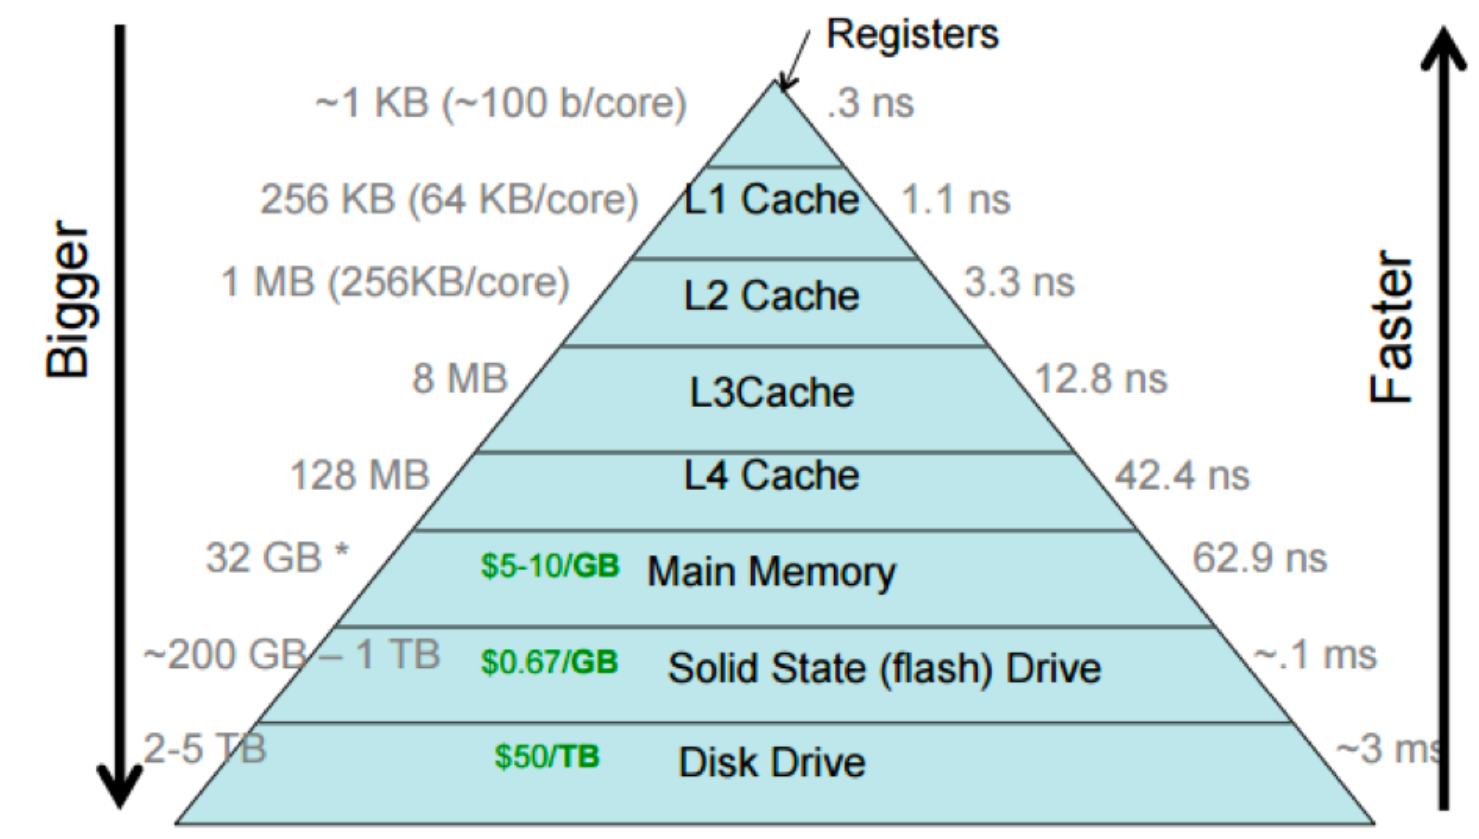
\includegraphics[width=1\linewidth]{content/OS_Internals/img/memory.png}
    \end{minipage}
  \end{minipage}
\end{center}

La memoria principale e i registri sono gli unici supporti di memorizzazione a cui la CPU può accedere direttamente. L'unità di memoria vede solo un flusso di:

\begin{itemize}
  \item indirizzi + richieste di lettura, oppure
  \item indirizzo + dati e richieste di scrittura
\end{itemize}

La CPU può accedere ai registri in uno, o meno, cicli di clock. Tuttavia, quando la CPU preleva dati dalla memoria principale utilizza molti cicli di clock, causando uno \textbf{stall}.

La cache si trova tra la memoria principale e i registri e funge da buffer per i dati necessari; non vogliamo un collo di bottiglia.


Tutti questi livelli contengono una copia dello stesso sottoinsieme di dati.

\subsection{Località spaziale e località temporale}

\paragraph{Località spaziale:} La località spaziale significa che se leggo una variabile o un'istruzione in memoria, tutti i dati vicini hanno un'alta probabilità di essere prelevati; pertanto quando leggo, leggo in blocchi e memorizzo tutti i dati in una memoria più veloce.\newline
\textbf{Località temporale:} La località temporale significa che se leggo una variabile, la probabilità di riutilizzarla è alta; pertanto la mantengo nella memoria cache.


\begin{figure}[htbp]
  \centering
  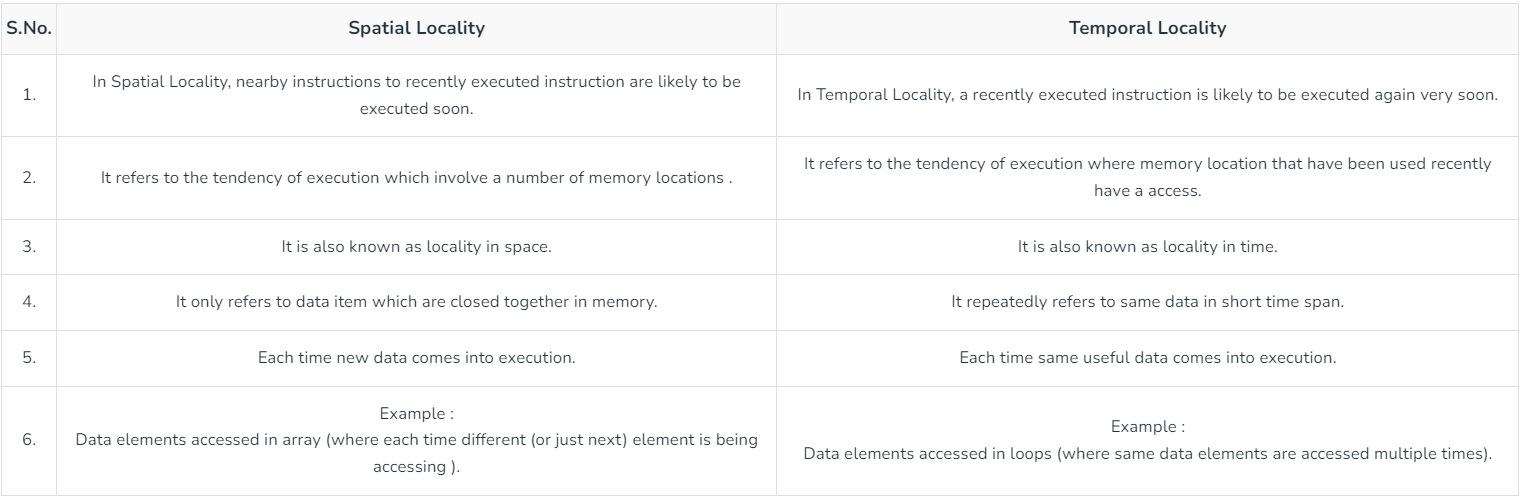
\includegraphics[width=0.9\linewidth]{content/OS_Internals/img/spatial.png}
\end{figure}

\newpage
\section{Problema della riallocazione}

Si presenta il problema di riallocazione: l'indirizzo deve essere scalato a quello reale.
Come si può risolvere?

\begin{itemize}
  \item Si guardando i riferimenti e calcolo l'indirizzo. Difficile
  \item Carico gli indirizzi così come sono. Fattibile utilizzando l'hardware.
\end{itemize}

Utilizzando l'hardware, base e limit, prima di arrivare al bus inseriamo un sommatore e in assembly non cambia nulla.

\section{Protezione}


\begin{center}
  \begin{minipage}{1\linewidth}
    % Primo blocco: 50% dello spazio per il codice
    \begin{minipage}{0.55\linewidth}
      Quando un programma è diventato un processo, tutti o gran parte dei suoi dati sono memorizzati nella memoria principale. Abbiamo bisogno di un modo per:

      \begin{itemize}
        \item Suddividere la memoria tra tutti i processi;
        \item Garantire che un processo possa accedere solo agli indirizzi del proprio spazio di indirizzamento\footnote{Lo spazio di indirizzamento, o address space, è una porzione di memoria cui un programma può utilizzare}.
      \end{itemize}

      Possiamo risolvere questi problemi utilizzando una coppia di registri \textbf{base} e \textbf{limite} che definiscono lo spazio di indirizzamento logico di un processo.

    \end{minipage}%
    \hfill
    \begin{minipage}{0.35\linewidth}
      \centering

      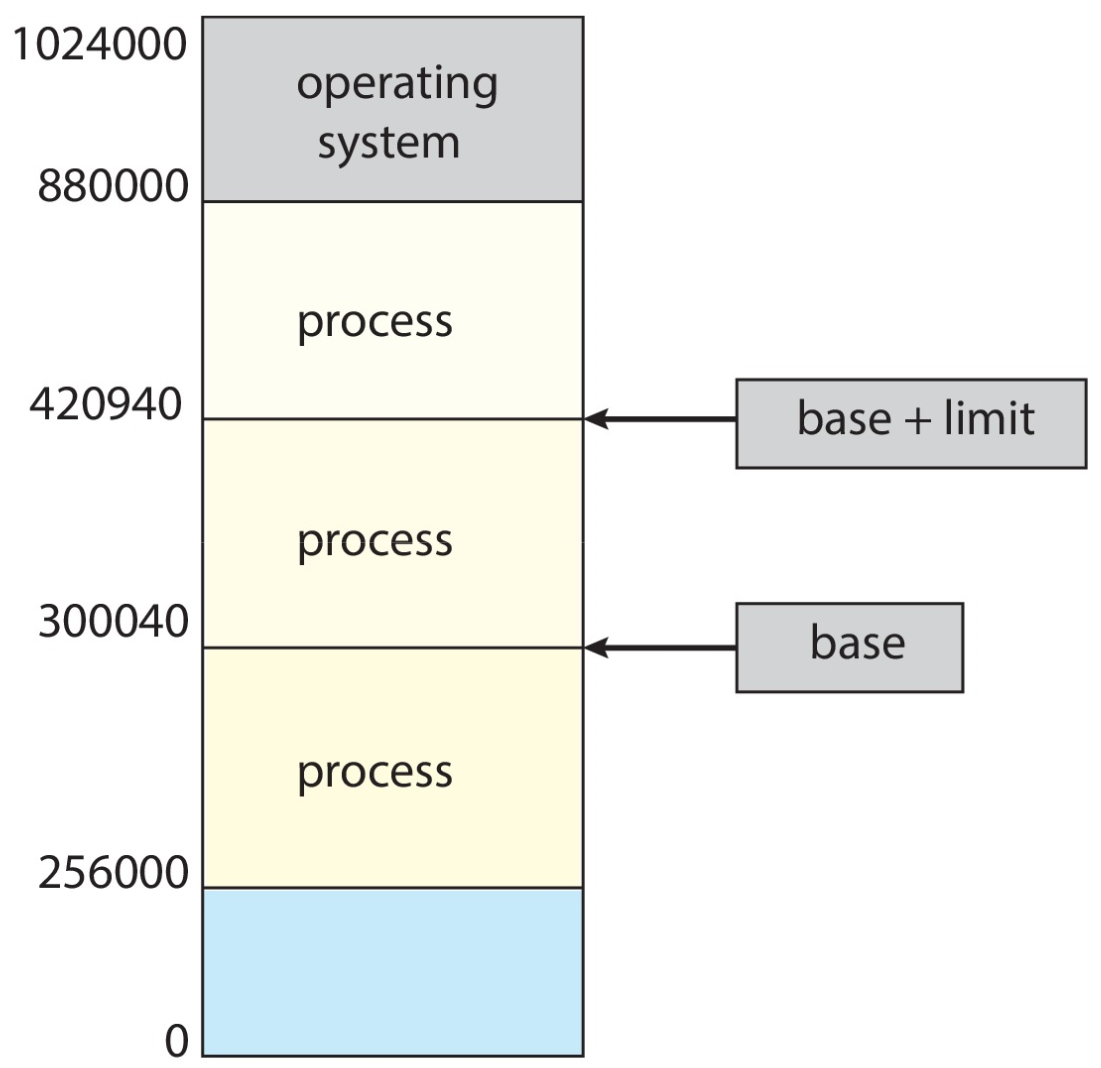
\includegraphics[width=1\linewidth]{content/OS_Internals/img/adsfcv.png}

    \end{minipage}
  \end{minipage}
\end{center}

\subsection{Protezione degli indirizzi hardware}


\begin{center}
  \centering
  \begin{minipage}{\linewidth}
    % Primo blocco: 50% dello spazio per il codice
    \begin{minipage}{0.50\linewidth}
      La CPU/OS deve verificare ogni accesso alla memoria generato in modalità utente per
      assicurarsi che sia compreso tra base e limite per quell'utente.


      Le istruzioni per caricare i registri base e limite sono privilegiate.
    \end{minipage}% <-- IMPORTANTE: il simbolo % qui evita spazi bianchi extra
    \hfill
    \begin{minipage}{0.4\linewidth}
      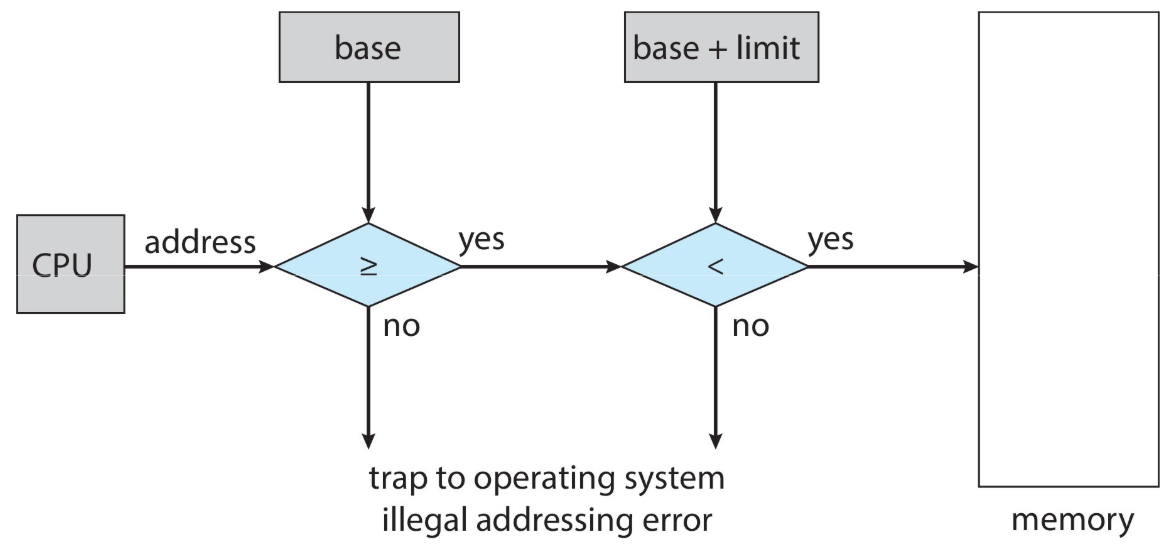
\includegraphics[width=1\linewidth]{content/OS_Internals/img/ikadsuhc.png}

    \end{minipage}
  \end{minipage}
\end{center}




\section{Binding degli indirizzi}

Quando scriviamo un programma C, vogliamo utilizzare indirizzi simbolici e vogliamo che sia il compilatore a trasformarlo in indirizzi relativi.
Il linker decide di riallocare a valori assoluti.

Inoltre non ci vogliamo preoccupare di dove si trovi la variabile in memoria, sappiamo solo che è in memoria.

\begin{itemize}
  \item Gli indirizzi nel codice sorgente sono tipicamente simbolici;
  \item Gli indirizzi nel codice compilato vengono legati a indirizzi rilocabili, es. «14 byte dall'inizio di questo modulo» invece di «byte 14»;
  \item Il linker o il loader legherà gli indirizzi rilocabili ad indirizzi assoluti;
  \item Ogni binding mappa uno spazio di indirizzamento in un altro.
\end{itemize}

Nel codice compilato vediamo quanta memoria è necessaria e non l'indirizzo codificato in modo fisso. Vogliamo un binding dinamico e non statico.


\subsubsection{Binding di istruzioni e dati in memoria}

% \begin{itemize}
%   \item compile time: Codice assoluto, si se lo sai già, altrimetni ricolabile. Sto generando l'eseguibile.
%   \item Load time: Fare il binding se gli inidirzzi non sono ancora decisi, generare un indirizzo assoluto o rilocabile e usato in fase di esecuzione. 
%   \item Execution time: Facciamo il binding sono quando il codice viene eseguito fino a che il processo viene mandato in esecuzione ed eventualmente spostato. La CPU al minimo deve offrire il Base register + limit register, deve dare supporto.
% \end{itemize}

Quando un programma viene avviato, il SO assegna una quantità di spazio al programma.

Il binding degli indirizzi di istruzioni e dati agli indirizzi di memoria può avvenire in tre momenti diversi:


\begin{center}
  \centering
  \begin{minipage}{\linewidth}
    % Primo blocco: 50% dello spazio per il codice
    \begin{minipage}{0.75\linewidth}

      \begin{itemize}
        \item \textbf{Tempo di compilazione:} Se la posizione in memoria è nota a priori, può essere generato codice assoluto; è necessario ricompilare il codice se la posizione iniziale cambia. Utilizzato nei sistemi embedded o nei sistemi in cui i task sono noti a priori e sono in numero ridotto. Sto generando l'eseguibile;

        \item \textbf{Tempo di caricamento:} Deve essere generato codice rilocabile se la posizione in memoria non è nota al momento della compilazione. Strategia ampiamente utilizzata nei vecchi SO o in sistemi semplici come le lavastoviglie...

        \item \textbf{Tempo di esecuzione:} Il binding viene ritardato al runtime se il processo può essere spostato durante l'esecuzione da un segmento di memoria a un altro; richiede supporto hardware (es. registri base e limite) ed è lo standard de facto per i SO moderni.

      \end{itemize}
    \end{minipage}% <-- IMPORTANTE: il simbolo % qui evita spazi bianchi extra
    \hfill
    \begin{minipage}{0.2\linewidth}
      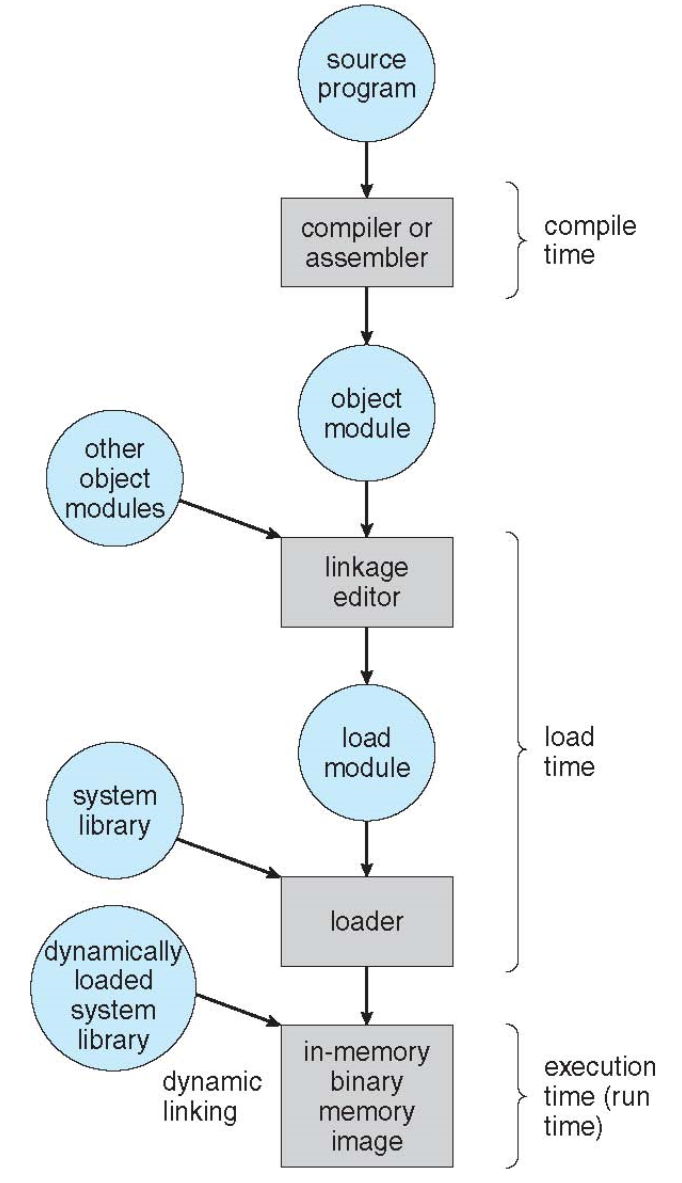
\includegraphics[width=1\linewidth]{content/OS_Internals/img/rwefbg.png}
      \captionof{figure}{Elaborazione in più fasi di un programma utente}
    \end{minipage}
  \end{minipage}
\end{center}


\section{Memory Management Unit - MMU}
Ho bisogno di un modo per passare dalla memoria virtuale alla memoria hardware e viceversa, soprattutto quando gli indirizzi sono diversi in fase di esecuzione. Introduciamo il concetto di \textbf{processo di binding}.


\subsection{Spazio di indirizzamento logico vs. fisico}
Il concetto di spazio di indirizzamento logico legato a un separato \textbf{spazio di indirizzamento fisico} è centrale per una corretta gestione della memoria.

\begin{itemize}
  \item \textbf{Indirizzo logico} - generato dalla CPU; detto anche \textbf{indirizzo virtuale};
  \item \textbf{Indirizzo fisico} - indirizzo visto dall'unità di memoria.
\end{itemize}

Gli indirizzi logici e fisici coincidono negli schemi di binding al tempo di compilazione e di caricamento, ma differiscono nello schema di binding al tempo di esecuzione.


\section{MMU}


\begin{center}
  \centering
  \begin{minipage}{\linewidth}
    % Primo blocco: 50% dello spazio per il codice
    \begin{minipage}{0.6\linewidth}

      Dispositivo hardware, all'interno della CPU, che al runtime mappa gli indirizzi virtuali, che troviamo nel codice assembler, in indirizzi fisici.
      Vi sono diverse tipologie di MMU, anche in base a quanto vogliamo far pagare il chip.

    \end{minipage}% <-- IMPORTANTE: il simbolo % qui evita spazi bianchi extra
    \hfill
    \begin{minipage}{0.35\linewidth}
      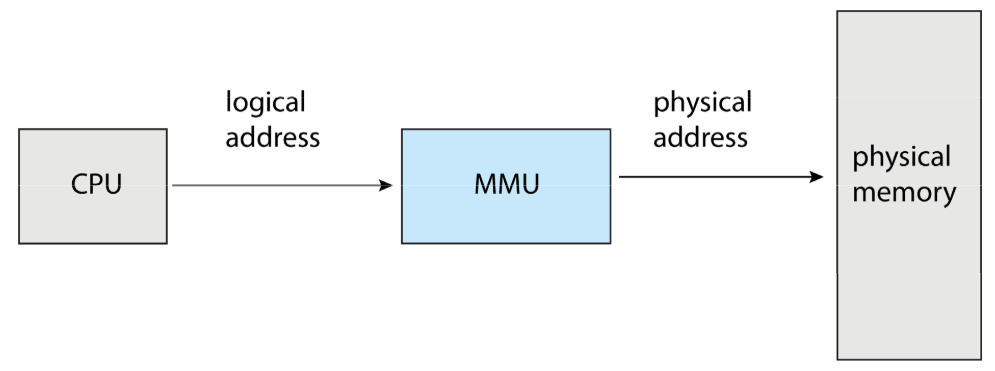
\includegraphics[width=1\linewidth]{content/OS_Internals/img/hnter.png}
    \end{minipage}
  \end{minipage}
\end{center}

\begin{center}
  \centering
  \begin{minipage}{\linewidth}
    % Primo blocco: 50% dello spazio per il codice
    \begin{minipage}{0.6\linewidth}

      Il registro base ora si chiama registro di rilocazione. Il valore nel registro di rilocazione viene aggiunto a ogni indirizzo
      generato da un processo utente nel momento in cui viene inviato alla memoria.

      Questo componente è composto da un sommatore ed un comparatore per bloccare il programma se vuole utilizzare spazi non facenti parti della sua address space.

    \end{minipage}% <-- IMPORTANTE: il simbolo % qui evita spazi bianchi extra
    \hfill
    \begin{minipage}{0.35\linewidth}
      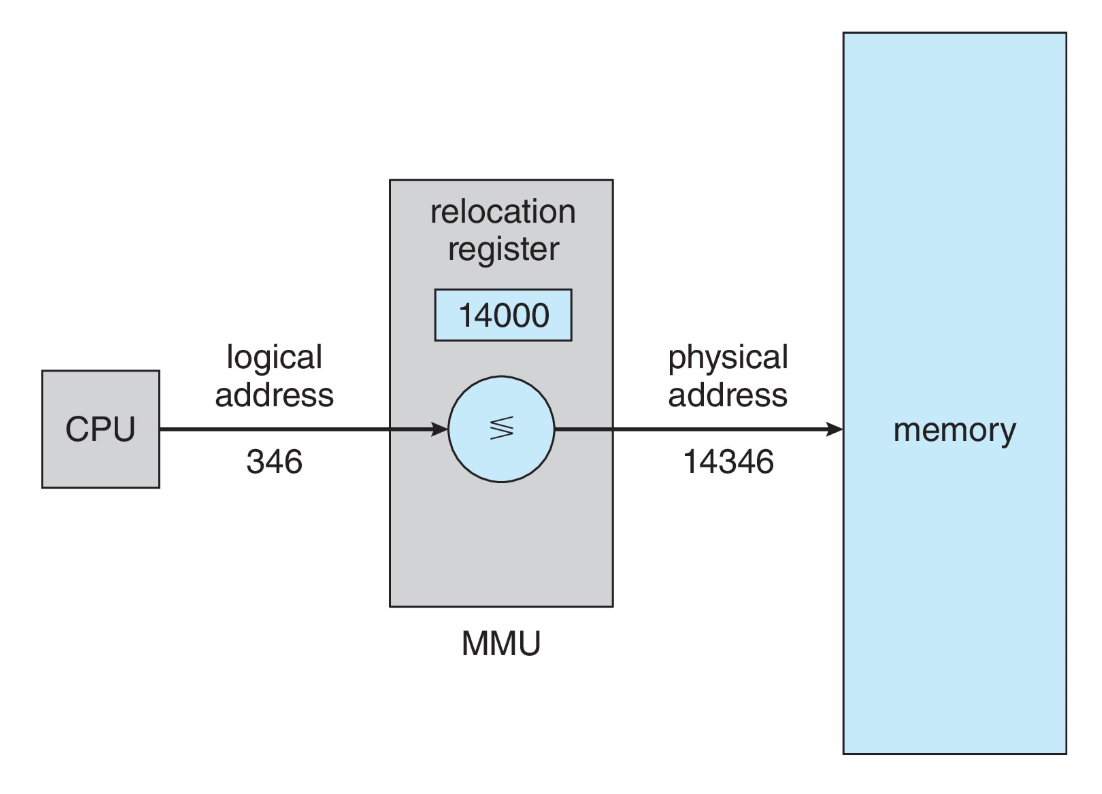
\includegraphics[width=1\linewidth]{content/OS_Internals/img/mmuu.png}
    \end{minipage}
  \end{minipage}
\end{center}


Il programma utente lavora con indirizzi logici; \textbf{non vede mai i veri indirizzi fisici}. Se si stampa l'indirizzo di una variabile in un programma C, viene stampato il valore logico e non il valore fisico reale!

\subsection{Registro di riallocazione}
Se abbiamo una MMU basta su Relocation register, gli indirizzi logici sono calcolati al volo. Viene utilizzato quando si vuole ritardare il binding fino alla fase di esecuzione.

Oltre che al relocation register ci sono anche altri modi per caricare nuovi processi in memoria: \textbf{Dynamic loading}  e \textbf{dynamic linking}

\subsection{Caricamento dinamico}
% il pgm non è detto che può stare tutto in memoria. e non è detto che lo voglio tutto subito in memoria.
% perché? spero una parte o tutto non mi serva più (è fatta in sequenza cencetto di località soazione e temprale).

% Non solo, 10K istruzioni, e parti completamente non utilizzate! ho deciso di sottoutilizzare il pgm oppure per righe di codice per errori etc

% perché non carichiamo solo quando una routine viene chiamata? 

% Poi ci consenza di non caricare le cose che non ci servo, ma il loader deve intervenire qunado serve e il file deve essere possibile caricarlo in momenti diversi(vedi il formato)
% Utile quanndo il codice è grande e quando statisticamente alcune parti non venfono utilizzate.


% Per quanto riguarda il linking, cosa significa? Il linker fa statico o dimatico?\newline

L'intero programma non deve necessariamente essere tutto in memoria per essere eseguito. Una routine, parte del programma, non vorremmo venisse caricata finché non viene chiamata.
Questo migliora l'utilizzo dello spazio in memoria. Il loader perciò deve intervenire quando vogliamo caricare nuove porzioni di codice.
Questo fa si che il programma deve essere organizzato ed avere un formato specifico.

Il SO può aiutare fornendo librerie per implementare il caricamento dinamico.


% \subsection{static linking}

% Le lib se sono statiche le agganci tutte. Difetto eseguibili grossi.

% \subsection{dynamic linking}
% Non fai tutto i link, ti tieni degli indizizzi non risolti (eg non sai la pintf etc) quando li saprai in fase di load o fase di esecuzione.

% cosa c'è al posto di printf, si mette un indizzo ad una routine , stoub, che fa finta di essere la routne e una volta arrivata li viene rimpizzata con la printf vera.

% Utile per le librerie! è utile per le shared librery, una sola copia in memoria e tutti la vedono: tutti la trovano già caricata MA spazio di indirizzamento condiviso!!
% Problema del versioning delle liberie shared, normalmente basta aggiornare.

\subsection{Linking Statico vs Dinamico}
\textbf{Linking statico} - librerie di sistema e codice di programma sono tutti combinati dal linker nell'immagine del programma binario in fase di compilazione. Problema: grandi eseguibili.

\noindent\textbf{Linking dinamico} - il linking è rinviato fino alla fase di esecuzione del programma.\newline
\noindent
\begin{tcolorbox}
  \textbf{Nota:} Le DLL possono avere le due varianti: load-time dynamic linking (caricamento all'avvio) o run-time dynamic linking (caricamento su richiesta durante l'esecuzione)
\end{tcolorbox}

\begin{center}
  \centering
  \begin{minipage}{\linewidth}
    % Primo blocco: 50% dello spazio per il codice
    \begin{minipage}{0.6\linewidth}

      Non tutti gli indirizzi sono risolti prima dell'esecuzione, pensiamo ad esempio alla printf, possiamo assumere che molti porgrammi in esecuzione possono volerla utilizzare.
      Per questo motivo teniamo ancora indirizzi non risolti e inseriamo piccolo frammento di codice, chiamati \textit{stub}, utilizzato per individuare la routine di libreria residente in memoria.
      A runtime lo stub, che faceva finta di essere la routine corretta, viene sostituita con l'indirizzo della routine corretta e la esegue a runtime.

      Il sistema operativo verifica se la routine si trova nello spazio di indirizzamento del processo e, in caso contrario, la aggiunge.

    \end{minipage}% <-- IMPORTANTE: il simbolo % qui evita spazi bianchi extra
    \hfill
    \begin{minipage}{0.35\linewidth}
      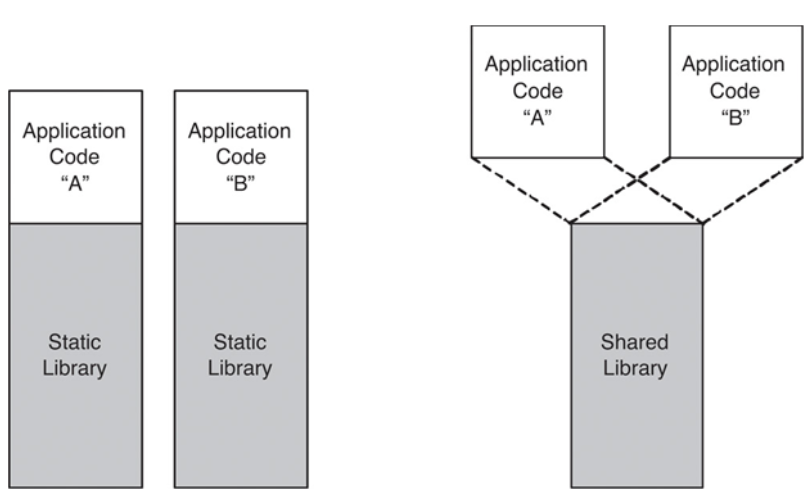
\includegraphics[width=1\linewidth]{content/OS_Internals/img/ddl.png}
      \captionof{figure}{File .dll}
    \end{minipage}
  \end{minipage}
\end{center}


\paragraph{}
\textbf{Vantaggio}: Il dynamic linking è particolarmente utile per le librerie, il sistema è anche visto come ``shared libraries'' (librerie condivise); questo consente di ottenere programmi di dimensioni ridotte poiché le librerie sono condivise tra più programmi.
Tutti i programmi, tranne il primo che la caricherà, la troveranno già in memoria.

Questo metodo offre inoltre un ulteriore vantaggio: quando Windows aggiorna una libreria, è necessario ricompilare solamente quella e non tutte le altre applicazioni che la utilizzano.


\textbf{Problemi}: Spazio condiviso e versioning delle librerie, normalmente viene risolto tramite l'aggiornamento di queste ultime.


% ------------- inizio BOH ----------

% \section{Excutable file}

% è un file binario e non di testo, con 1 header, codice e dati e sa symbol table

% Linking: prndi un insieme di pgm (file oggetto) e crea un file caricabile (image) nel fare questo risolvi i simboli
% Loading: copiare l'eseguibile in memoria e magari agganciarlo con pezzo già caricate (eg shared library) e aggiorarre gli indizzi se sevono.

% \section{Classic unix}

% Unix usa gcc.
% Il linker vive dentro gcc
% il loader è parte di una system call Exec
%  static loading

% \section{Dynaimc loading} 


% \section{Programm-controlled dynamic loading}
% Il programma si gestisce il load e sostituisce lui. Serve solo la LOAD e non la printf!
% Eg la printf nella prima chiamata carica la printf e tutte le altre volte invece già presa dalla memoria.


% \subsection{linker assidted dynamic loading}

% Lo stab myPrintf fa subito la load e in qualche modo il loader/linker verrà poi sostituita in esecuzione, l'indirizzo cambia e c'è più inerzione con il sistema operativo.
% Cmabia la responsabilità di chi fa qualcosa

% \section{shared library}
% Alcuni pgm usano la stessa fuznone, quindi facciamo un load automatico e il linker non la risolve. se il loader è già in memoria la carico altrimenti lo eseguito


% \section{dynamic linking}
% Il linking non è fatto in memoria completo e verrà fatto quello completo a livello di esecuzione.

% Solo dire caricamenot dinamico degli indizii un po' alla volta. 
% il dynamic loading significa solo che il programma non è caricato tutto in una botta ma un po' alla volta.


% \section{Dynamic shared library}
% sono le dll che usano sia dynamic loading e linking. Che sono l'altro apsetto della medaglia diq aundo abbiamo deciso che ci sono delgi indizii fisici e logici.

% ----------- fine BOH-------------

\section{Allocazione dei programmi}

A questo punto dobbiamo parlare di dove effetticamente vengono allocati i programmi in memoria, e di come viene creato lo spazio di indirizzamento.
Nella memoria centrale va inserito tutto, dal sistema operativo ai processi utente. Solitamente il SO si prende una parte di RAM in alto o in basso dato che lui non parteciperà al gioco dell'allocazione e deallocazione della memoria

\subsection{Allocazione contigua}

Vogliamo gestire efficientemente la memoria principale perché deve supportare sia il SO che i processi utente ed è una risorsa limitata; deve essere allocata in modo efficiente.

L'allocazione contigua è uno dei primi metodi: array e liste concatenate.

\paragraph{}

La memoria principale è solitamente suddivisa in due partizioni:

\begin{itemize}
  \item Sistema operativo residente, solitamente collocato in memoria bassa con il vettore degli interrupt;
  \item I processi utente sono collocati in memoria alta
\end{itemize}

% \textbf{sotto 0 non vai, 1M? se il limite è 500K, è un rischio, leggi qualcosa che non dovresti}
% \textbf{ma se corrompi qualcosa?} 

% \textbf{C'era il limitation register, ora c'è altro.}


\begin{center}
  \centering
  \begin{minipage}{\linewidth}
    % Primo blocco: 50% dello spazio per il codice
    \begin{minipage}{0.6\linewidth}

      Ogni processo è contenuto in una singola sezione contigua di memoria.

      Il relocation register viene utilizzato per proteggere i processi utente l'uno dall'altro e per impedire modifiche al codice e ai dati del sistema operativo.

    \end{minipage}% <-- IMPORTANTE: il simbolo % qui evita spazi bianchi extra
    \hfill
    \begin{minipage}{0.35\linewidth}
      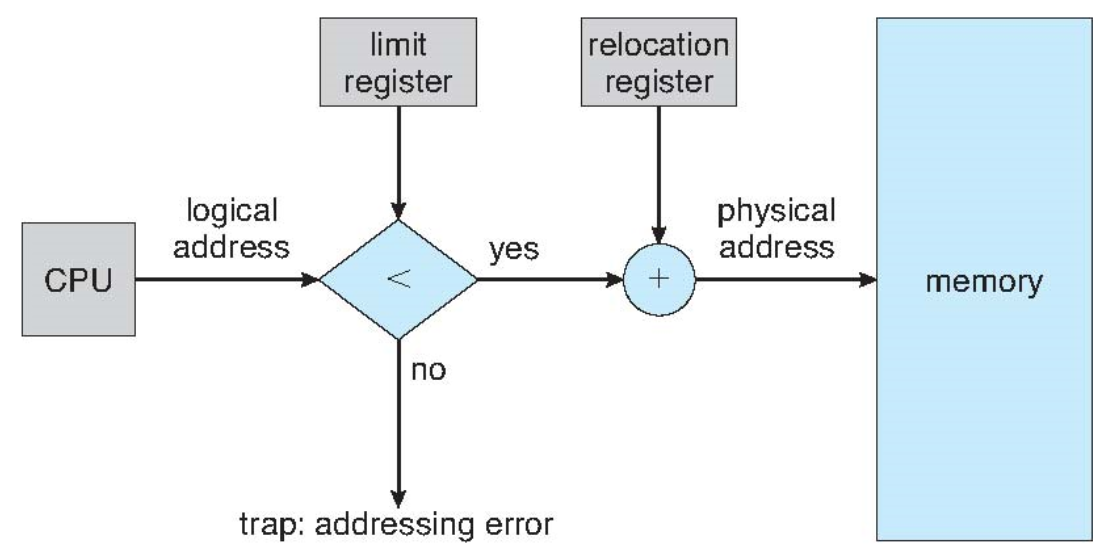
\includegraphics[width=1\linewidth]{content/OS_Internals/img/fbs.png}
    \end{minipage}
  \end{minipage}
\end{center}

\begin{itemize}
  \item Il base register contiene il valore del più piccolo indirizzo fisico
  \item Il limit register contiene l'intervallo degli indirizzi logici - ogni indirizzo logico deve essere inferiore al registro limite
  \item La MMU mappa dinamicamente gli indirizzi logici
\end{itemize}


\subsection{Partizione variabile}

Il SO può decidere l'allocazione a partizioni multiple. Il grado di multiprogrammazione è limitato dal numero di partizioni.

\begin{itemize}
  \item \textbf{Partizione variabile} - dimensioni per l'efficienza (dimensionate in base alle necessità del processo).
  \item \textbf{Buco} - blocco di memoria disponibile; buchi di varie dimensioni sono dispersi nella memoria. Indesiderato; idealmente si vuole un blocco contiguo di memoria disponibile.
\end{itemize}

\begin{center}
  \centering
  \begin{minipage}{\linewidth}
    % Primo blocco: 50% dello spazio per il codice
    \begin{minipage}{0.6\linewidth}

      Quando un processo arriva, gli viene allocata memoria da un buco sufficientemente grande da contenerlo; quando un processo termina e libera la sua partizione, le partizioni libere adiacenti vengono unite. Tutto ciò è gestito dal sistema operativo che mantiene informazioni su:

    \end{minipage}% <-- IMPORTANTE: il simbolo % qui evita spazi bianchi extra
    \hfill
    \begin{minipage}{0.35\linewidth}
      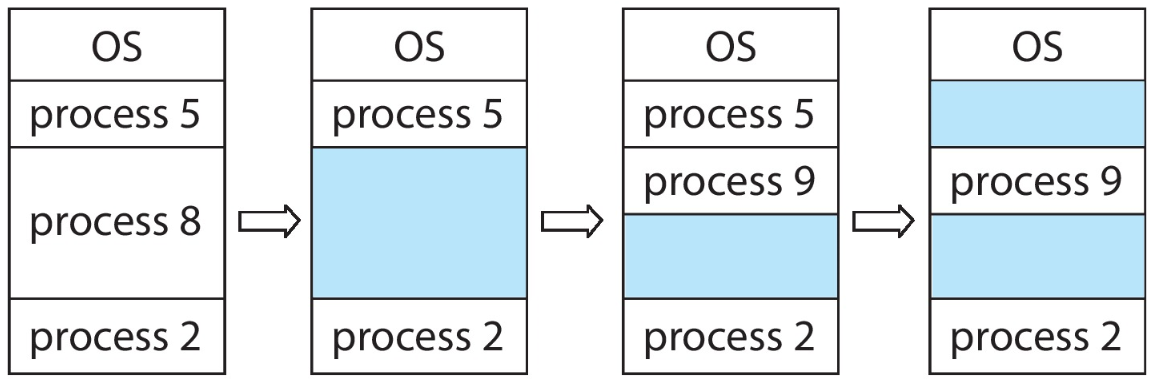
\includegraphics[width=1\linewidth]{content/OS_Internals/img/jyrt.png}
    \end{minipage}
  \end{minipage}
\end{center}

\begin{itemize}
  \item partizioni allocate
  \item partizioni libere (buchi)
\end{itemize}


\newpage
\subsection{Problema dell'allocazione dinamica della memoria}
Come soddisfare una richiesta di dimensione n da una lista di buchi liberi?

\begin{itemize}
  \item \textbf{First-fit}: Alloca il primo buco sufficientemente grande
        \begin{itemize}
          \item[] Può produrre molti piccoli buchi residui
        \end{itemize}

  \item \textbf{Best-fit}: Alloca il buco più piccolo sufficientemente grande; deve scorrere l'intera lista, salvo che sia ordinata per dimensione

        \begin{itemize}
          \item[] Produce il buco residuo più piccolo, che potrebbe non essere più riempito.
        \end{itemize}

  \item \textbf{Worst-fit}: Alloca il buco più grande; deve anch'esso scorrere l'intera lista
        \begin{itemize}
          \item[] Produce il buco residuo più grande, che può essere riempito da altri processi.
        \end{itemize}
\end{itemize}

First-fit e best-fit sono migliori di worst-fit in termini di velocità e utilizzo della memoria.
Per decidere tra Best e Worst fit andrebbero fatti test sul campo.

\subsection{Frammentazione}

% \textbf{Frammentazione: si lascianod dei residuzi sono troppo piccoli e tanti. Memoria frammentata a pezzettini.
% Stiamo parlando di frammentazione esterne
% }

% \textbf{fino a qui, introduzione tra indirizzi logici e fisici e abbaimo parlato di allocazione contigua
% allocazione di partizioni contigue (un solo intervallo fisico
% variabile: qualcuno è più grossa e qualcono è più piccola)
% nella deframmentazione però ci possono essere dei Job che non possono essere spostati
% }

\begin{center}
  \centering
  \begin{minipage}{\linewidth}
    % Primo blocco: 50% dello spazio per il codice
    \begin{minipage}{0.6\linewidth}

      \paragraph{Frammentazione esterna} - esiste sufficiente spazio di memoria totale per soddisfare una richiesta, ma non è contiguo. Sia la strategia first-fit che best-fit causano frammentazione esterna.

    \end{minipage}% <-- IMPORTANTE: il simbolo % qui evita spazi bianchi extra
    \hfill
    \begin{minipage}{0.35\linewidth}
      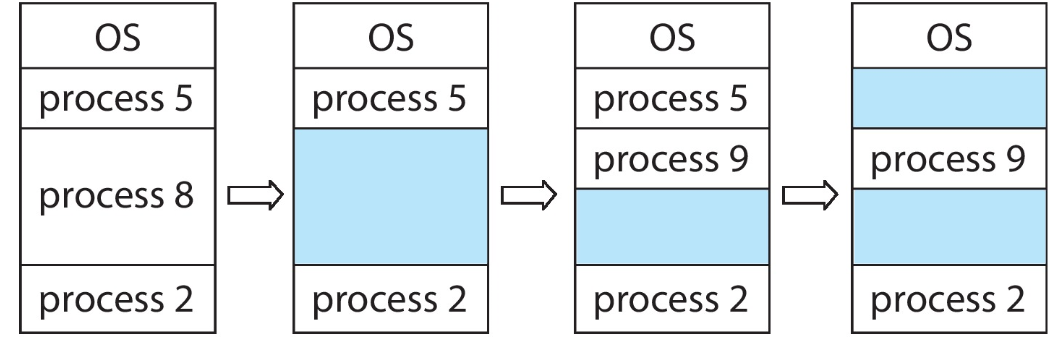
\includegraphics[width=1\linewidth]{content/OS_Internals/img/mkjhg.png}
    \end{minipage}
  \end{minipage}
\end{center}




\begin{center}
  \centering
  \begin{minipage}{\linewidth}
    % Primo blocco: 50% dello spazio per il codice
    \begin{minipage}{0.6\linewidth}

      \paragraph{Frammentazione interna} - la memoria allocata può essere leggermente più grande di quella richiesta; la dimensione minima è definita dal SO e la differenza tra la dimensione del programma C e questa dimensione minima è detta frammentazione interna. L'uso della partizione dinamica per assegnare spazio al processo può risolvere questo problema.

    \end{minipage}% <-- IMPORTANTE: il simbolo % qui evita spazi bianchi extra
    \hfill
    \begin{minipage}{0.35\linewidth}
      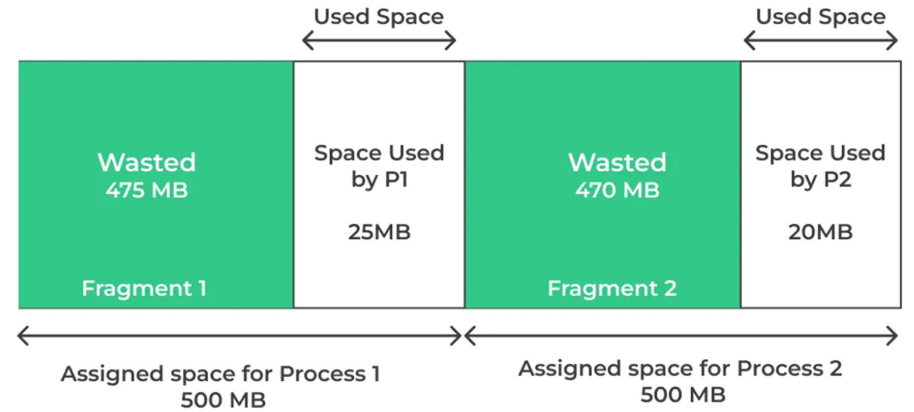
\includegraphics[width=1\linewidth]{content/OS_Internals/img/mht.png}
    \end{minipage}
  \end{minipage}
\end{center}

È sensato pensare che allocando N blocchi, la metà sono frammentati. E.g. 100 blocchi, 50 frammentati, 50 utilizzati, frammentazione del ~50\% (thumb roule).

\subsection{Compattazione}
Si riduce la frammentazione esterna tramite la \textbf{compattazione}: il contenuto della memoria viene riorganizzato in modo da raccogliere tutta la memoria libera in un unico blocco contiguo. La compattazione è possibile solo se la rilocazione è dinamica e viene eseguita al tempo di esecuzione.

Esempio: La cosa migliore sarebbe trasferire tutti i processi da un'altra parte, questo implica
avere altra RAM la quale avrei utilizzato se l'avessi avuta. Posso utilizzare il disco ma questo
significa che non potrei utilizzare il  pc.

Inoltre si presenta il problema dell'I/O: se un processo è "waiting for IO",
non posso spostarlo perché altrimenti l'I/O non saprebbe dove inviare i dati.

Solutioni: 1. Evitare che il processo venga spostato, la cui conseguenza è una
deframmentazione non ottimale;

2. Spostare comunque il programma utilizzando un buffer, anche se questo comporta
un tempo complessivo di spostamento più lungo. Spostare la memoria da utente a kernel fatto all'inizio di "waiting for IO".
% \textbf{Esempio: ristsitemare i mobili e l'alloggio è sempre pieno. la cosa migliore è portare tutto fuoi e poi rimetto dentro.
% Quando si può fare nel cotesto dei processo? Tutti i processi fermi a patto del kernel, 
% se avessi ram allora l'avrei utilizzata, c'è il disco ma dovrei stare fermi 1 ora.}

% \textbf{c'è il problema dell' IO -> un processo è fermo per "waiting for IO" e non posso spostarlo perché i dispoositivi IO sono molto più lenti.
% Fai altro nel mentre! IO significa c'è qualcuno che sta spostando dati da qualche posizione in ram o vicecersa.}

% \textbf{Se lo sposto (metà del trasloco) e sposto da tuttalatra parre i dati di altri programmi, l'impresa di traslochi si trova basita %:)
% }
% \textbf{soluzioni: 1. evita che il processo venga spostato, consegnuenza deframmentazione NON ottimale
% 2. spostalo ma prendi precauzioni, come fare? mettiamo un buffer anche se il tempo compessivo di spostamento è più lungo -> chiamata bufferizzazioine.
% M M IO,  sposta dalla memroa user 1000 a memoria kernel ed è rapido fatto all'inizo di waiting for IO. Eg 7MB da spostare li sposto in memoria kernel, svincolare il processo di. BUFFERIZZAZIONE
% }
% \textbf{concusione: si può fare la frammentazione, ma si può fare altro! deframmentare implica aspettare tempo!
% }

\paragraph{}
Sebbene la tecnica di compattazione sia molto utile per migliorare l'utilizzo della memoria e ridurre la frammentazione esterna, il problema è che durante il processo viene sprecata una grande quantità di tempo e la CPU rimane inattiva, riducendo l'efficienza complessiva del sistema.

\section{Paginazione}

Supponiamo di consentire che lo spazio di indirizzamento fisico di un processo possa essere non contiguo: il vantaggio è maggiore. In questo modo, al processo viene allocata memoria fisica ogni volta che la memoria principale è disponibile. Evitiamo la frammentazione esterna e blocchi di memoria di dimensioni variabili, sono della stessa dimensione.

Il processo di paginazione consiste nel dividere la memoria fisica in blocchi di dimensione fissa chiamati \textbf{frame}; la dimensione è una potenza di 2, compresa tra 512 byte e 16 MiB. Anche la memoria logica viene divisa in blocchi della stessa dimensione chiamati \textbf{pagine}.\newline
\noindent
\begin{tcolorbox}
  \textbf{Nota:} a questo punto è indifferente parlare di SSD o RAM, è la stessa cosa; cambiano solo la latenza e la volatilità.
\end{tcolorbox}

Questo permette di tenere traccia di tutti i frame liberi e consente di eseguire un programma di dimensione N pagine, trovando N frame liberi e caricando il programma. Per fare ciò dobbiamo impostare una tabella delle pagine per tradurre gli indirizzi logici in fisici.\newline
La frammentazione interna è ancora presente.

Per trovare i frame liberi possiamo utilizzare una free-list oppure un vettore chiamato bitmap.


\subsection{Schema di traduzione degli indirizzi}

L'indirizzo (virtuale) generato dalla CPU è suddiviso in:


\begin{minipage}{0.9\linewidth}
  % Primo blocco: 50% dello spazio per il codice
  \begin{minipage}{0.7\linewidth}
    \begin{itemize}
      \item \textbf{Numero di pagina (p)} - usato come indice in una tabella delle pagine che contiene l'indirizzo base di ogni pagina nella memoria fisica;
      \item \textbf{Offset di pagina (d)} - combinato con l'indirizzo base definisce l'indirizzo di memoria fisica inviato all'unità di memoria.
    \end{itemize}
  \end{minipage}% <-- IMPORTANTE: il simbolo % qui evita spazi bianchi extra
  \hfill
  \begin{minipage}{0.25\linewidth}
    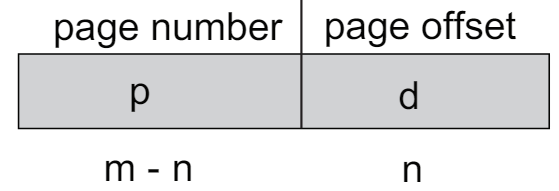
\includegraphics[width=1\linewidth]{content/OS_Internals/img/yuj,.png}
  \end{minipage}
\end{minipage}


Per un dato spazio di indirizzamento logico $2^m$ e dimensione di pagina $2^n$.

\section{Hardware di paginazione}

Abbiamo quasi annullato il problema della frammentazione dato che tutti i processi
ora possono prendere la stessa dimensione della pagina, e non importa se sono contigue o no.


% \textbf{
%   Logical memory, 40MB lo diviamo in 4, cerchiamo 4 in memoria:
%   non sono contigui
%   non importa nulla dell'ordine
%   Se facciamo questo, abbiamo quasi annualto il probelma della frammentaizne: perché
%   se tutti i processi giocano con pagine della stessa paginazione, possiamo vedere la memoria
%   fisica come una lista !  La page table sta in memoria del kernel.
% }


\begin{center}
  \centering
  \begin{minipage}{\linewidth}
    % Primo blocco: 50% dello spazio per il codice
    \begin{minipage}{0.48\linewidth}
      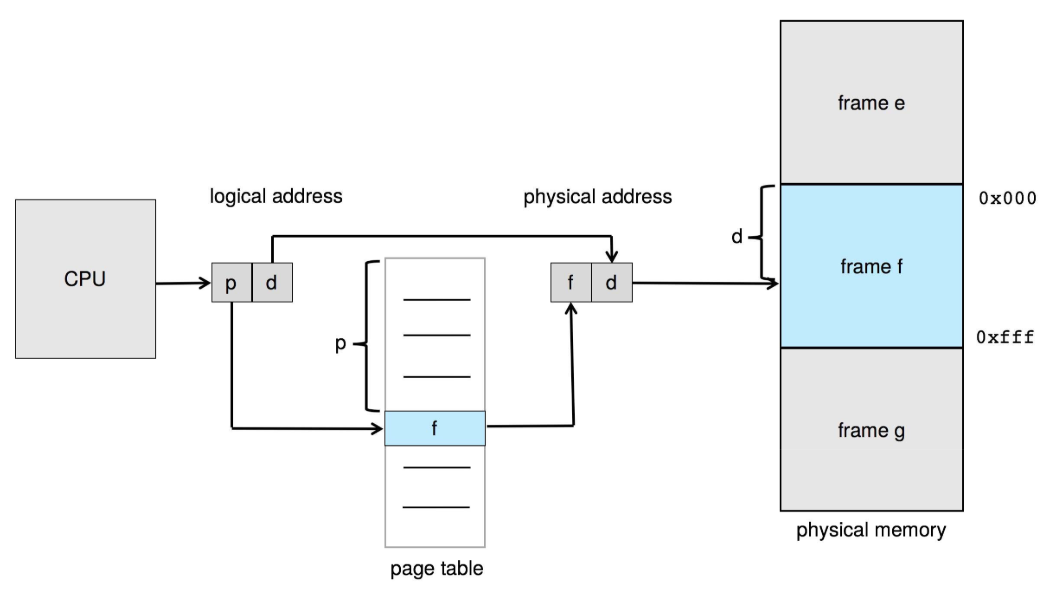
\includegraphics[width=0.95\linewidth]{content/OS_Internals/img/nfg.png}

    \end{minipage}% <-- IMPORTANTE: il simbolo % qui evita spazi bianchi extra
    \hfill
    \begin{minipage}{0.48\linewidth}
      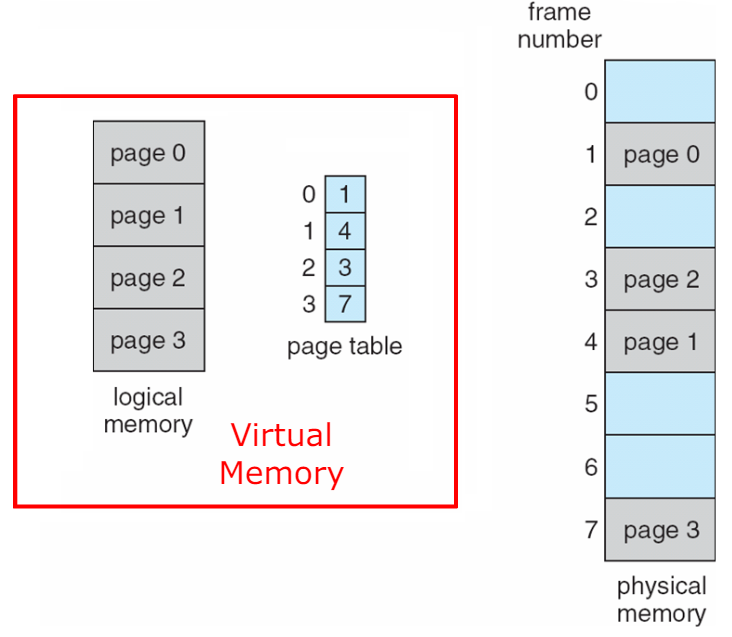
\includegraphics[width=0.95\linewidth]{content/OS_Internals/img/dsf.png}
      \captionof{figure}{Modello di paginazione della memoria logica e fisica}
    \end{minipage}
  \end{minipage}
\end{center}


\subsubsection{Esempio di paginazione}

Indirizzo logico: n = 2 (bit di offset), n-m = 3 (bit di pagina). Con una dimensione di pagina di 4 byte e una memoria fisica di 32 bit ($2^m$ = 8 pagine).

\begin{figure}[htbp]
  \centering
  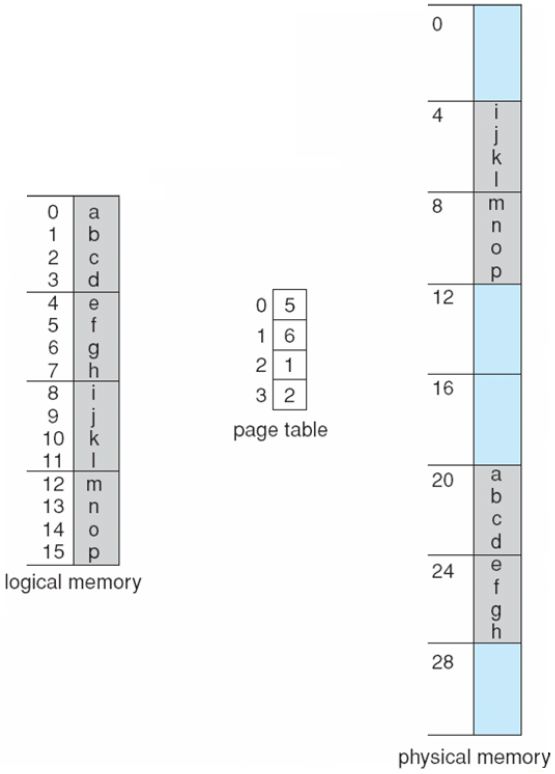
\includegraphics[width=0.35\linewidth]{content/OS_Internals/img/jmy.png}
\end{figure}


\subsubsection*{Paginazione - Calcolo della frammentazione interna}

Dimensione pagina = 2.048 byte; dimensione processo = 72.766 byte; si usano 35 pagine + 1.086 byte, la frammentazione interna è 2.048 - 1.086 = 962 byte.

Caso peggiore = dimensione frame - 1 byte; in media frammentazione = 1/2 dimensione frame.

\paragraph{}
Quindi, frame di dimensione ridotta consentono una piccola frammentazione interna... ma la dimensione della tabella delle pagine aumenta perché ogni tabella delle pagine, per processo, occupa memoria: dimensione pagina piccola = moltissime pagine = molta memoria allocata per tracciare le pagine e non disponibile per i task utente/SO.

Le dimensioni delle pagine sono cresciute nel tempo:

\begin{itemize}
  \item Solaris supporta due dimensioni di pagina - 8 KB e 4 MB
  \item Win10 supporta due dimensioni di pagina - 4 KB e 2 MB
  \item Linux supporta due dimensioni di pagina - 4 KB e dimensione huge page personalizzata
\end{itemize}

\begin{figure}[htbp]
  \centering
  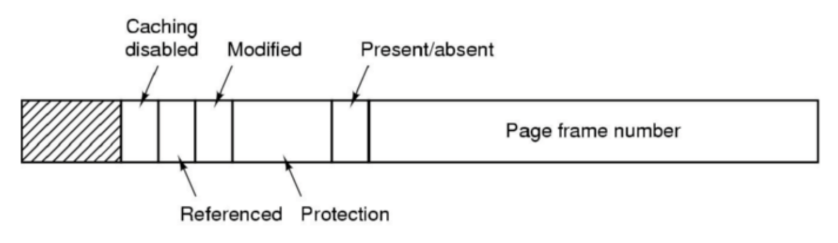
\includegraphics[width=0.5\linewidth]{images/OS_internals/Main-memory/MM-esempio4.png}
\end{figure}

Sappiamo, dato l'architettura e il funzionamento della memoria e dei processori, che
non possiamo allocare vettori di dimensioni arbitrarie, ma dobbiamo utilizzare potenze di 2.

A questo punto, essendo che abbiamo celle disponibili, possiamo
memorizzare dati aggiuntivi. Ad esempio, la protection bit per indicare se
il frame è read-only o se è anche permesso fare accessi read-write.

% \textbf{Essendo che gli array utilizzano multipli di $2^x$ byte, non possiamo fare un array
% di 22, facciamolo di 32 e memorizziamo altri dati nelle celle disponibili}

\subsection{Quante pagine?}
Supponiamo una dimensione di pagina di 4KB (212 byte) e una CPU hardware a 32 bit. La voce della tabella delle pagine è pari a 32 bit. $2^{32}$ pagine, ciascuna da 4KiB, per un totale di memoria indirizzabile pari a 16 TiB ($2^{12} * 2^{10}$, dove il primo termine rappresenta gli indirizzi di paginazione e il secondo l'offset).\newline
Altro esempio:

\begin{center}
  \centering
  \begin{minipage}{\linewidth}
    % Primo blocco: 50% dello spazio per il codice
    \begin{minipage}{0.7\linewidth}
      \begin{itemize}
        \centering
        \item[] m = lunghezza indirizzo = 8 bit.
        \item[] n = $log_2(\text{dimensione pagina})$ = $log_2(32 \text{ byte})$ = 5 bit di offset.
        \item[] m - n = 3 = numero di pagine che posso indirizzare.
      \end{itemize}
      Riducendo la dimensione della pagina si possono indirizzare più pagine e l'offset diminuisce. Normalmente m = 32 e la dimensione della pagina è 4KiB, come nell'esempio precedente.

    \end{minipage}% <-- IMPORTANTE: il simbolo % qui evita spazi bianchi extra
    \hfill
    \begin{minipage}{0.25\linewidth}
      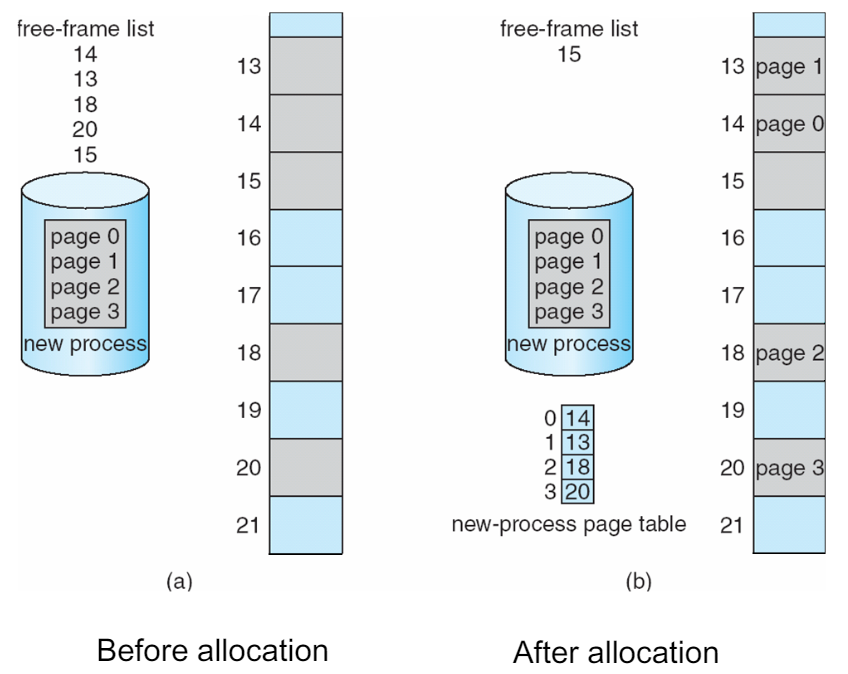
\includegraphics[width=1\linewidth]{content/OS_Internals/img/yrtjn.png}
      \captionof{figure}{Frame liberi}
    \end{minipage}
  \end{minipage}
\end{center}

\subsection{Implementazione della page table}
La tabella delle pagine, come detto in precedenza, è mantenuta nella memoria principale. È il principale "artefatto" della gestione della memoria virtuale:

\begin{itemize}
  \item[] Il registro base della tabella delle pagine (Page-table base register - PTBR) punta alla tabella delle pagine
  \item[] Il registro di lunghezza della tabella delle pagine (Page-table length register - PTLR) indica la dimensione della tabella delle pagine
\end{itemize}

In questo schema ogni accesso a dati o istruzioni richiede \textbf{due accessi alla memoria}! Uno per la tabella delle pagine e uno per i dati o l'istruzione.

Il problema del doppio accesso alla memoria può essere risolto tramite l'uso di una speciale cache hardware ad accesso rapido chiamata \textit{translation look-aside buffer}, \textbf{TLB}.

\paragraph{}
Sfrutta la \textbf{località temporale}: la tendenza dei programmi a utilizzare ripetutamente gli stessi dati nel corso della loro esecuzione.

\subsection{Soluzione hardware - Translation Look-Aside Buffer}

% \textbf{
%   TBL unica, 
%   le pagine table, una per processo
%   e ogni volta che c'è context switch la TLB deve ripartirre da zero oppure fai essitere + processi
%   ma significa che metto 3 cose al posto di 2 (il pid  ASID)
% }

La TLB è una cache univoca per tutte le page table. Il primo apporccio potrebbe essere
quello di svuotare la TLB ad ogni context switch, ma questo è inefficiente.

\begin{center}
  \centering
  \begin{minipage}{\linewidth}
    % Primo blocco: 50% dello spazio per il codice
    \begin{minipage}{0.6\linewidth}
      Invece di svuotare la TLB, memorizziamo anche \textbf{identificatori dello spazio di indirizzamento di un dato processo} (ASID) in ogni voce del TLB.

      I TLB sono tipicamente piccoli, da 64 a 1024 voci, ma più veloci; sono quindi una cache completamente associativa.

      In caso di TLB miss, il valore viene caricato nel TLB per un accesso più rapido la volta successiva; le politiche di sostituzione devono essere considerate; alcune voci possono essere fissate per un accesso rapido permanente.

    \end{minipage}% <-- IMPORTANTE: il simbolo % qui evita spazi bianchi extra
    \hfill
    \begin{minipage}{0.37\linewidth}
      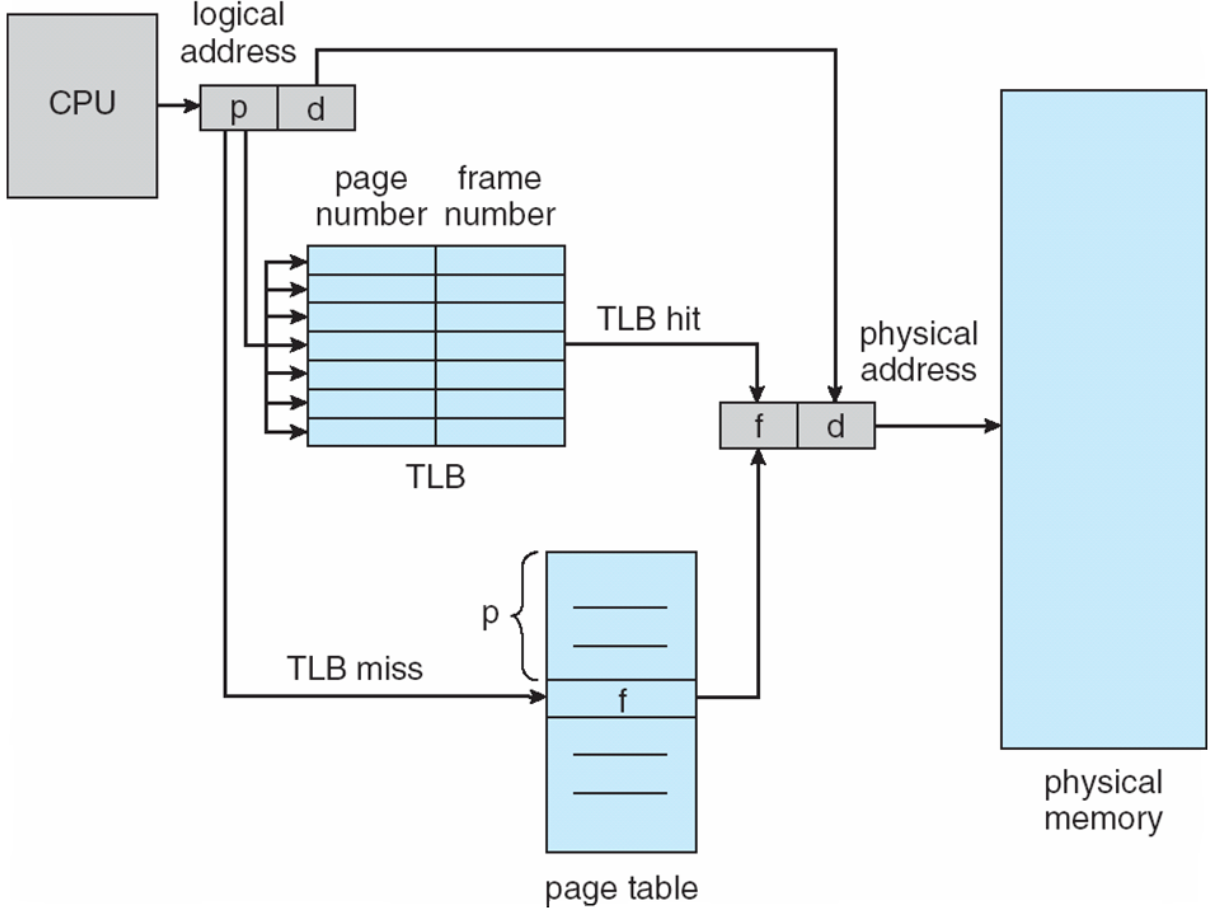
\includegraphics[width=1\linewidth]{content/OS_Internals/img/ythmu.png}
    \end{minipage}
  \end{minipage}
\end{center}


\begin{minipage}{0.95\linewidth}
  % Primo blocco: 50% dello spazio per il codice
  \begin{minipage}{0.6\linewidth}
    Non accelera tutto:

    \begin{itemize}
      \item Caso medio: accesso nel TLB + accesso in memoria per il dato;
      \item Caso peggiore: nessun dato nel TLB, quindi accesso in memoria per la tabella delle pagine + accesso in memoria per il dato.
    \end{itemize}
  \end{minipage}% <-- IMPORTANTE: il simbolo % qui evita spazi bianchi extra
  \hfill
  \begin{minipage}{0.37\linewidth}
    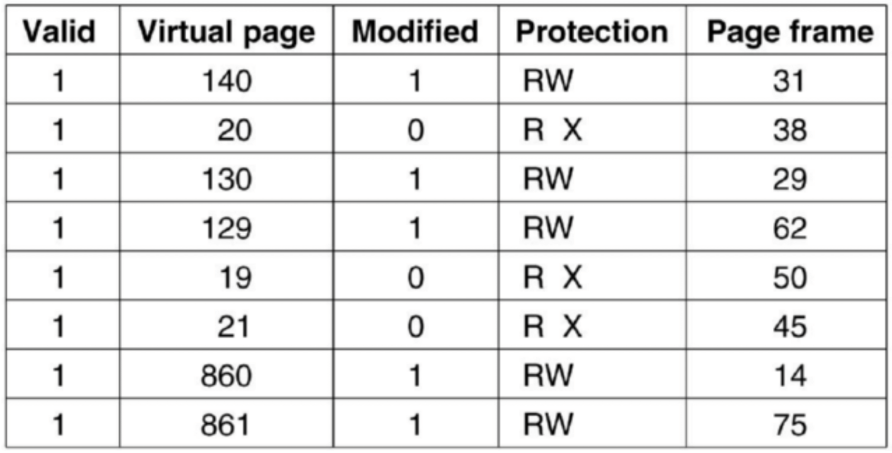
\includegraphics[width=1\linewidth]{images/OS_internals/Main-memory/MM-esempio5.png}
  \end{minipage}
\end{minipage}

Una volta riempita la TLB, dobbiamo utilizzare algoritmi per decidere quale voce sostituire in caso di TLB miss.
Sicuramente l'utilizzo di un valid-invalid bit per ogni voce del TLB è utile per identificare le voci che possono essere sovrascritte.

% \textbf{
%   se è piena? si gioca con gli algoritmi di sostituzione
% }

% \textbf{
%   cosa serve di mettere in cache se è un errore, cosa serve quindi il bit valid or invalid?
%   se cerco una casella libera vado a cercare gli zeri
% }

\subsection{Tempo di accesso effettivo}

% \textbf{Domande da esame:}

\textbf{Hit ratio} - percentuale delle volte in cui un numero di pagina viene trovato nel TLB. Un hit ratio dell'80\% significa che troviamo il numero di pagina desiderato nel TLB l'80\% delle volte.

Supponiamo che siano necessari 10 nanosecondi per accedere alla memoria. Se troviamo la pagina desiderata nel TLB, un accesso alla memoria mappata richiede 10 ns; altrimenti servono due accessi alla memoria, quindi 20 ns.

\paragraph{}
\textbf{Tempo di accesso effettivo} (EAT) = 0,80 x 10 + 0,20 x 20 = 12 nanosecondi, il che implica un rallentamento del 20\% nel tempo di accesso.

Considerando un hit ratio più realistico del 99\%, EAT = 0,99 x 10 + 0,01 x 20 = 10,1 ns, il che implica solo l'1\% di rallentamento nel tempo di accesso.

\section{Codice C e page fault}

Immagina di avere la RAM piena, con solo una pagina libera, e in questa pagina vogliamo fare questo:

\begin{minted}{c}
int main(){
    int[128,128] data;

    ...

    for (j = 0; j <128; j++)
        for (i = 0; i < 128; i++)
            data[i,j] = 0;
 
    //quanti page fault? 128 * 128 = 16384

    ...

    for (i = 0; i < 128; i++)
        for (j = 0; j < 128; j++)
            data[i,j] = 0;

    //quanti page fault? solo 128

}   
\end{minted}

\begin{center}
  \centering
  \begin{minipage}{\linewidth}
    % Primo blocco: 50% dello spazio per il codice
    \begin{minipage}{0.6\linewidth}
      \textbf{Page fault} - Un page fault si verifica quando un programma tenta di accedere a dati o codice che si trovano nel suo spazio di indirizzamento, ma non sono attualmente nella RAM del sistema.

      Quando si accede a qualcosa nella RAM, il SO carica un blocco di dati dall'SSD nella RAM. Nel primo caso il SO carica un blocco ma il codice C usa solo la prima colonna; nel secondo caso il SO carica un blocco di dati e ne usa tutta la colonna.

    \end{minipage}% <-- IMPORTANTE: il simbolo % qui evita spazi bianchi extra
    \hfill
    \begin{minipage}{0.37\linewidth}
      \centering
      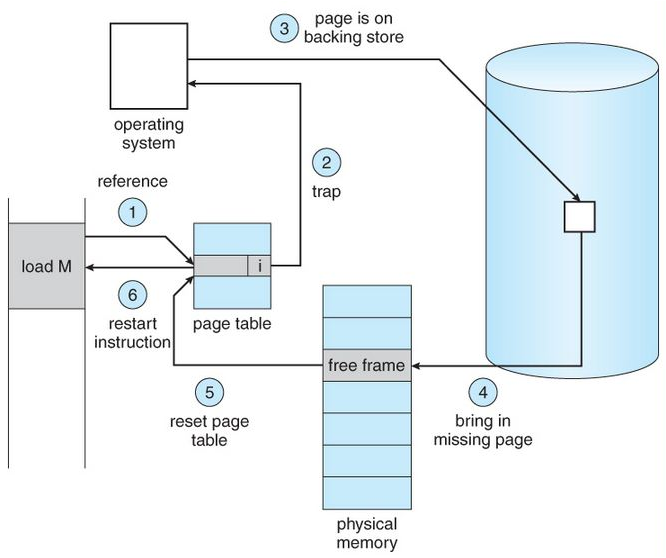
\includegraphics[width=0.6\linewidth]{content/OS_Internals/img/bnetg.png}
      \captionof{figure}{Page fault}\end{minipage}
  \end{minipage}
\end{center}


\section{Page fault}

\begin{center}
  \centering
  \begin{minipage}{\linewidth}
    % Primo blocco: 50% dello spazio per il codice
    \begin{minipage}{0.6\linewidth}
      \paragraph{Cos'è un page fault?} I dati sono tipicamente memorizzati in memorie non volatili, grandi e lente, e poi caricati nella RAM; ciò significa che i dati necessari per l'esecuzione (una pagina) possono esistere solo nella memoria secondaria a causa del caricamento dinamico. Devono quindi essere caricati nella RAM, poi nella cache, poi nei registri: questo è un \textbf{page fault}!\newline
      Non possiamo eliminarlo, ma cerchiamo di mitigare questo evento lento.
    \end{minipage}% <-- IMPORTANTE: il simbolo % qui evita spazi bianchi extra
    \hfill
    \begin{minipage}{0.37\linewidth}
      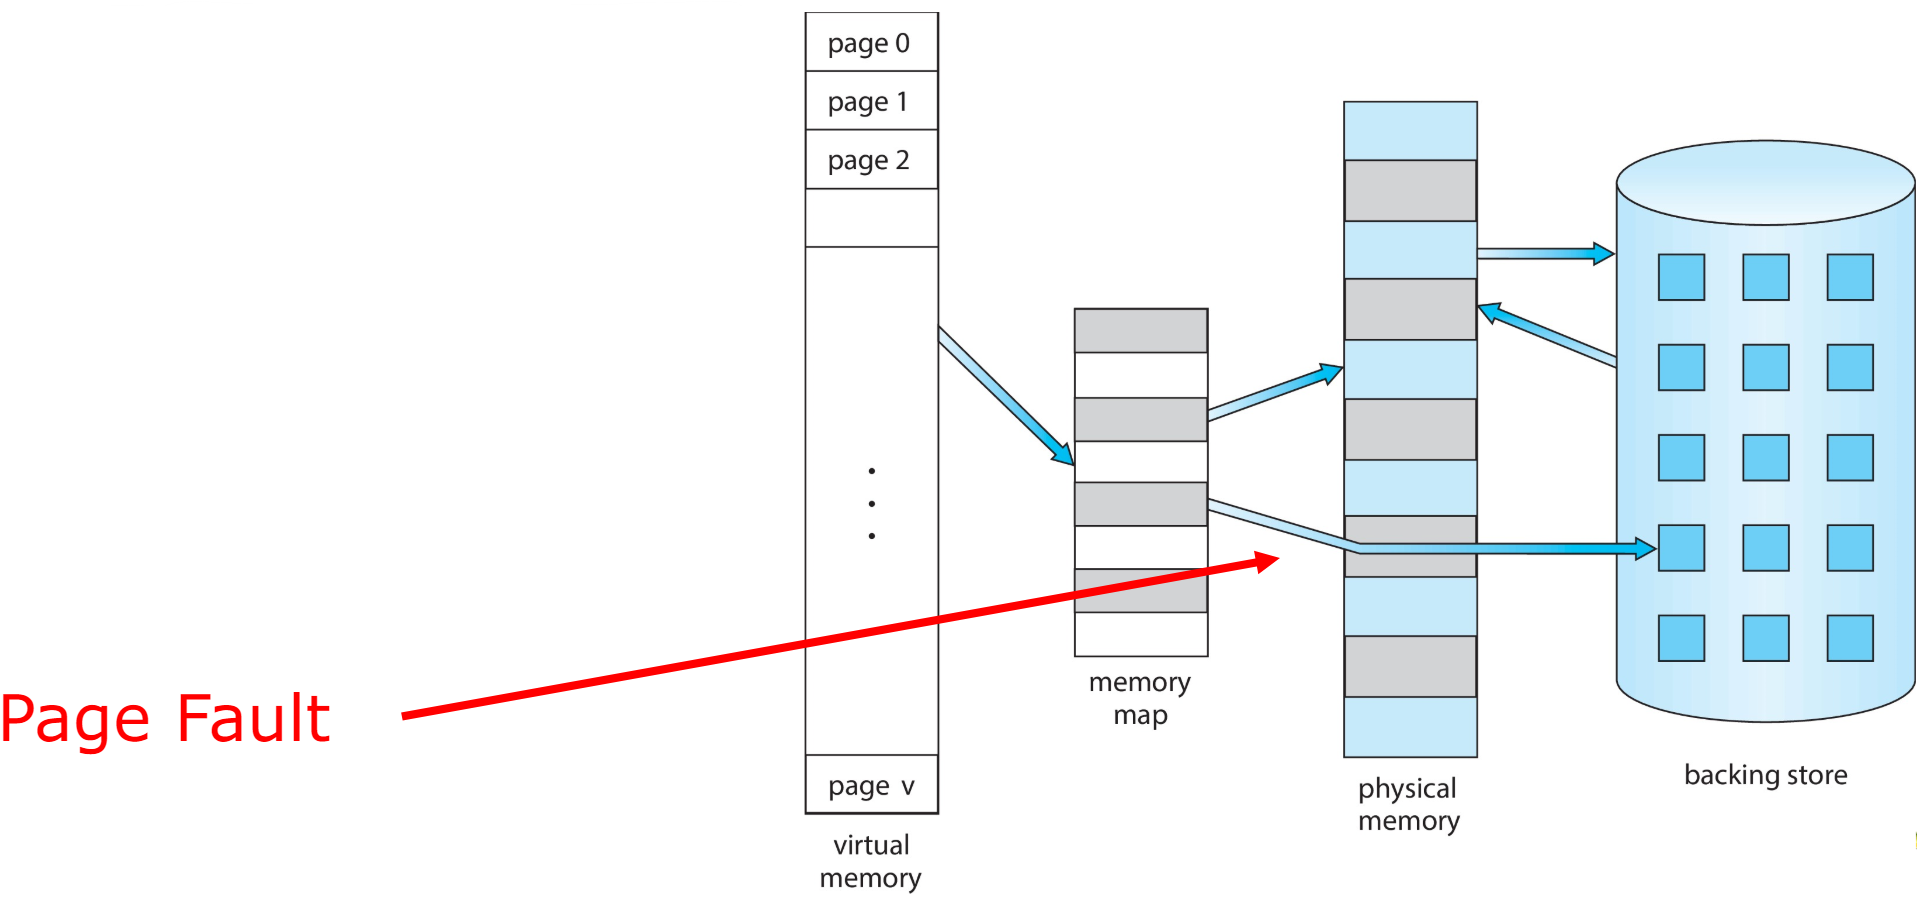
\includegraphics[width=1\linewidth]{content/OS_Internals/img/frsb.png}
      \captionof{figure}{Page fault}

    \end{minipage}
  \end{minipage}
\end{center}

\subsubsection{Contesto}

Il codice deve essere in memoria per essere eseguito,
ma l'intero programma è raramente utilizzato interamente per via della
gestione delle eccezioni, funzioni non utilizzate e larghe strutture dati.

Tutto il programma non è necessario allo stesso tempo.

Considera la possibilità di eseguire un programma parzialmente caricato:
il programma non è più vincolato dai limiti della memoria fisica, ogni programma
occupa meno memoria durante l'esecuzione, il che consente a più programmi di essere
eseguiti contemporaneamente, aumentando l'utilizzo della CPU e il throughput senza
aumentare i tempi di risposta o turnaround. Inoltre, è necessario meno I/O per
caricare o scambiare programmi in memoria, il che significa che ogni programma utente
viene eseguito più velocemente.\newline

Stiamo parlando di loading dinamico e non abbiamo bisogno che tutto il programma
sia tutto in RAM. La ram deve essere capiente abbastanza da contenre il kernel
+ la parte dei processi che stiamo eseguendo.

\subsubsection{Memoria virtuale}

\textbf{Virtual memory: } separazione tra memoria logica utente e memoria fisica;
solo una parte del programma deve essere in memoria per l'esecuzione; lo spazio
di indirizzamento logico può quindi essere molto più grande dello spazio di
indirizzamento fisico (RAM); consente la condivisione degli spazi di
indirizzamento da parte di più processi; consente una creazione di processi più
efficiente; più programmi in esecuzione contemporaneamente; meno I/O necessario
per caricare o scambiare processi in memoria.

\noindent\textbf{Virtual address space: } molto maggiore della memoria fisica;
visualizzazione logica di come il processo è memorizzato in memoria; di solito
inizia all'indirizzo 0 ma non è detto, con indirizzi contigui fino alla fine
dello spazio; nel frattempo, la memoria fisica è organizzata in frame di pagina;
la MMU deve mappare gli indirizzi logici a quelli fisici.

La virtual memory può essere implementata tramite: demand paging o demand segmentation.

% demand paging: quando acceso alle tabelle delle pagine o avviene la traduzione o che devo accedere ad una pagina che è ancora virtuale, non c'è ancora

\begin{center}
  \centering
  \begin{minipage}{\linewidth}
    % Primo blocco: 50% dello spazio per il codice
    \begin{minipage}{0.7\linewidth}
      Normalmente lo spazio di indirizzamento logico è progettato in modo che lo stack inizi all'indirizzo logico massimo e cresca "verso il basso", mentre l'heap cresce "verso l'alto". Questo massimizza l'utilizzo dello spazio degli indirizzi, lasciando uno spazio inutilizzato tra i due, noto come "buco". Non è necessaria memoria fisica fino a quando l'heap o lo stack non crescono fino a una nuova pagina. Ciò consente spazi di indirizzamento sparsi con buchi lasciati per la crescita, librerie dinamicamente collegate, ecc. Le librerie di sistema possono essere condivise tramite mappatura nello spazio di indirizzamento virtuale. La memoria condivisa può essere implementata mappando pagine in lettura-scrittura nello spazio di indirizzamento virtuale. Le pagine possono essere condivise durante fork(), accelerando la creazione dei processi.

    \end{minipage}% <-- IMPORTANTE: il simbolo % qui evita spazi bianchi extra
    \hfill
    \begin{minipage}{0.25\linewidth}
      \centering
      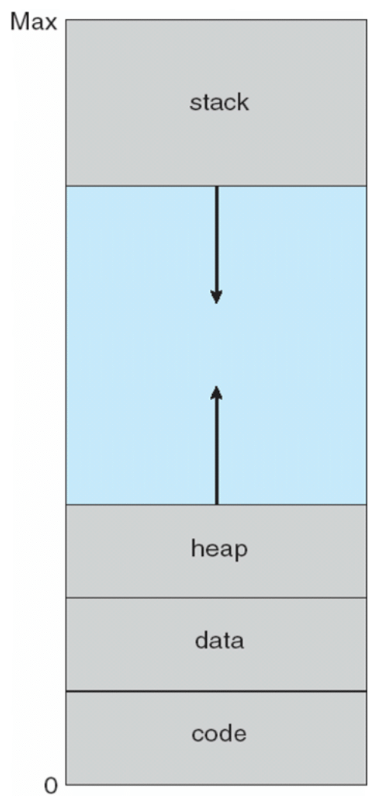
\includegraphics[width=0.3\linewidth]{images/OS_internals/Main-memory/MM-esempio6.png}
      \vspace{0.5cm}
      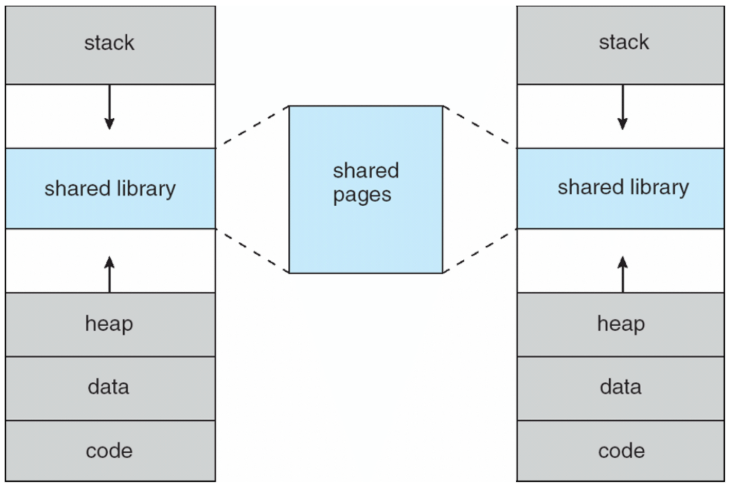
\includegraphics[width=1\linewidth]{images/OS_internals/Main-memory/MM-esempio7.png}
    \end{minipage}
  \end{minipage}
\end{center}

\subsubsection{Paginazione su Richiesta - Demand Paging}


\begin{center}
  \centering
  \begin{minipage}{\linewidth}
    % Primo blocco: 50% dello spazio per il codice
    \begin{minipage}{0.6\linewidth}
      Posso caricare un processo interamente in memoria al momento del caricamento, oppure posso caricare una pagina solo quando è necessaria. Il demand paging richiede meno I/O, non esegue I/O non necessario, richiede meno memoria, offre una risposta più rapida e consente più utenti. È simile a un sistema di paging con swapping.\newline

      Il demand paging consiste nel caricare la prima pagina del processo e di comportarsi
      come abbiamo fatto prima per i processi, swap in e swap out, ma lo fai a livello di pagina
      page in e page out.

      \textbf{Lazy swapper} non swappa mai pagine nella memoria fino a che quella pagina non è necessaria.


      \begin{tcolorbox}
        \textbf{Nota: } Uno swapper trasferisce in memoria/disco
        l'intero processo. Quando invece si trasferiscono solo le singole pagine
        (e non l'intero processo), si parla di pager e l'operazione si chiama
        paging.
      \end{tcolorbox}

    \end{minipage}% <-- IMPORTANTE: il simbolo % qui evita spazi bianchi extra
    \hfill
    \begin{minipage}{0.37\linewidth}
      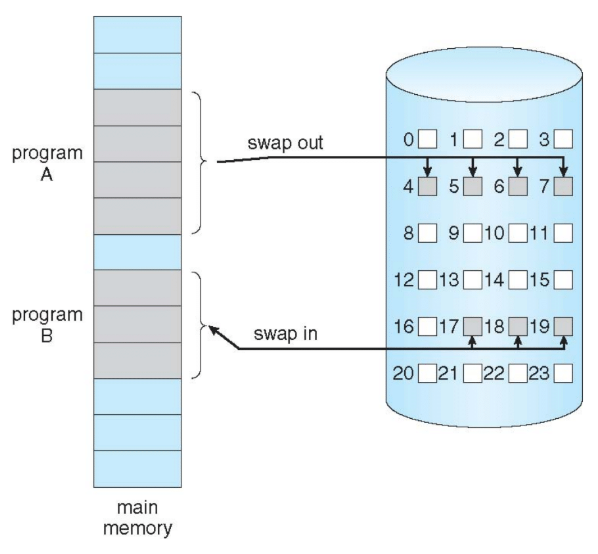
\includegraphics[width=1\linewidth]{images/OS_internals/Main-memory/MM-esempio8.png}
    \end{minipage}
  \end{minipage}
\end{center}

\subsubsection{Concetti di Base}

Con lo swapping, il pager indovina quali pagine saranno utilizzate prima di essere nuovamente
scambiate. Invece, il pager porta in memoria solo quelle pagine necessarie. Come determinare
quel set di pagine? È necessaria una nuova funzionalità della MMU per implementare il demand paging.
Se le pagine necessarie sono già residenti in memoria (\textbf{Memory resident}), non c'è
differenza rispetto al non demanding paging.

Se la pagina necessaria NON è residente in memoria, è necessario rilevare e caricare la
pagina in memoria dallo storage senza modificare il comportamento del programma e senza
che il programmatore debba modificare il codice.


\subsection{Come rilevare i page fault?}

Possiamo usare un bit, \textbf{valid-invalid}, per tracciare se l'indirizzo è nella RAM o nella memoria secondaria.

\begin{tcolorbox}
  \textbf{Nota: } Vi è un problema dell'allineamento tra la memoria primaria e fisica.
\end{tcolorbox}

\begin{itemize}
  \item valido (1): indica che la pagina associata è nello spazio di
        indirizzamento logico del processo ed esiste già nella RAM;
  \item non valido (0): indica che la pagina non è nello spazio di
        indirizzamento logico del processo e non è nella RAM, il che significa che si
        verificherà un \textbf{page fault/trap nel kernel}. Inizialmente, sono tutte
        non valide.
\end{itemize}


\begin{center}
  \centering
  \begin{minipage}{0.85\linewidth}
    % Primo blocco: 50% dello spazio per il codice
    \begin{minipage}{0.48\linewidth}
      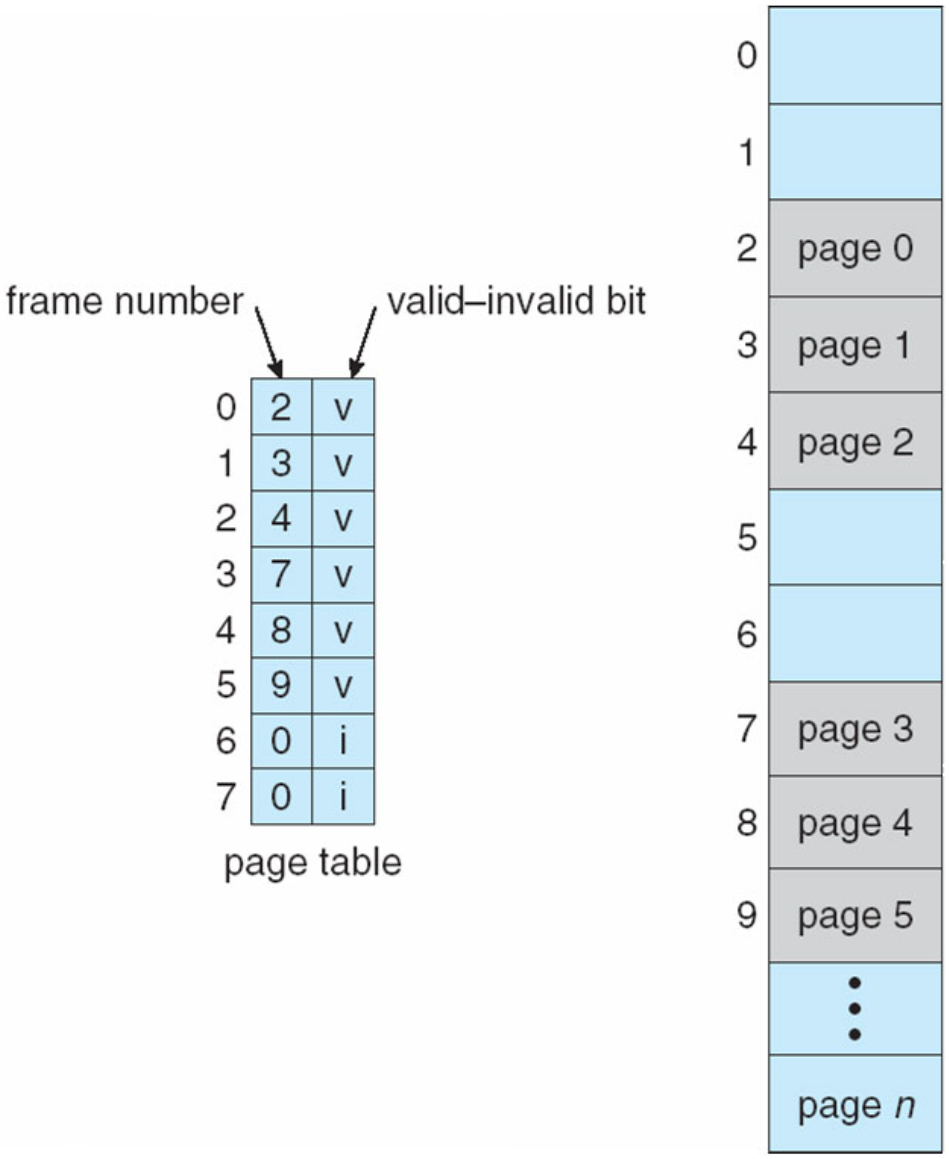
\includegraphics[width=0.55\linewidth]{content/OS_Internals/img/rfynhmg.png}

    \end{minipage}% <-- IMPORTANTE: il simbolo % qui evita spazi bianchi extra
    \hfill
    \begin{minipage}{0.48\linewidth}
      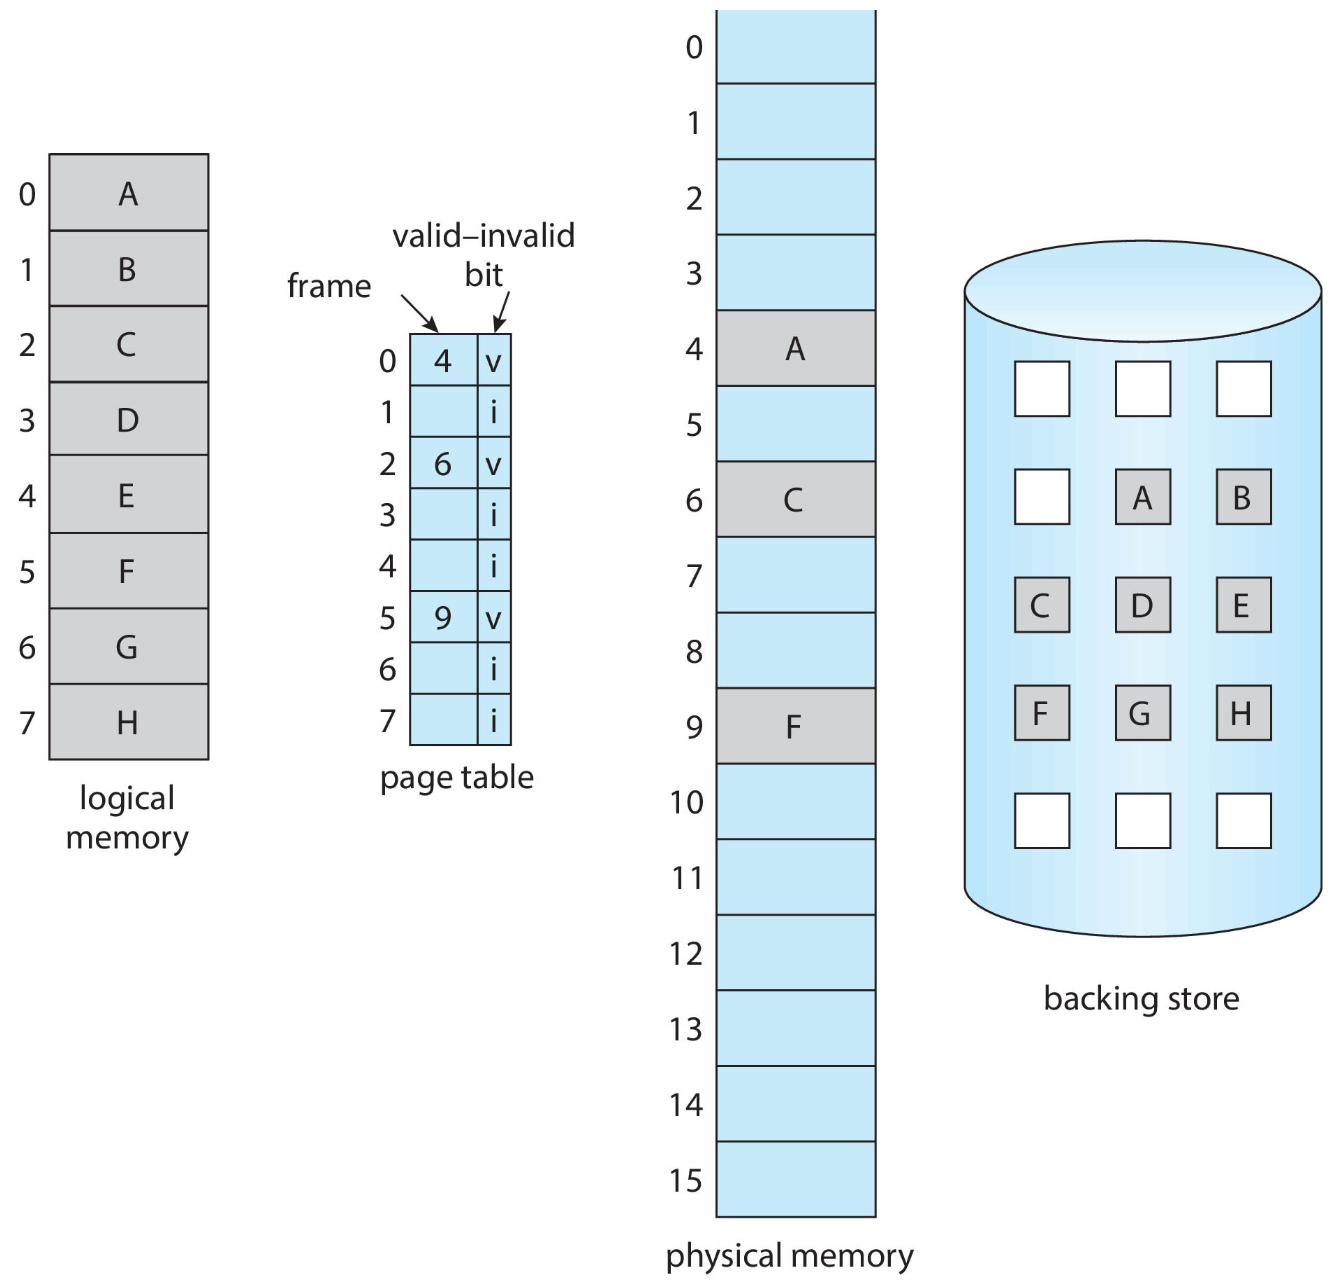
\includegraphics[width=0.7\linewidth]{content/OS_Internals/img/mhg.png}

    \end{minipage}
  \end{minipage}
\end{center}



\subsection{Passi nella gestione dei page fault}


\begin{minipage}{1\linewidth}
  % Primo blocco: 50% dello spazio per il codice
  \begin{minipage}{0.6\linewidth}
    \begin{enumerate}
      \item Se c'è un riferimento a una pagina (invalida), il primo riferimento a quella pagina genera un trap al sistema operativo = page fault;
      \item Il Sistema Operativo giarda un'altra tabella per decidere se:
            \begin{itemize}
              \item[] Riferimento non valido $\to$ abort
              \item[] Semplicemente non in memoria, deve essere caricata dal disco
            \end{itemize}
      \item Trovare un frame libero in memoria;
      \item Caricare la pagina nel frame tramite un'operazione disco pianificata, la parte più lenta del processo;
      \item Aggiornare le tabelle per indicare che la pagina è ora in memoria; impostare il bit valido = v;
      \item Riavviare l'istruzione che ha causato il page fault;
    \end{enumerate}
  \end{minipage}% <-- IMPORTANTE: il simbolo % qui evita spazi bianchi extra
  \hfill
  \begin{minipage}{0.36\linewidth}
    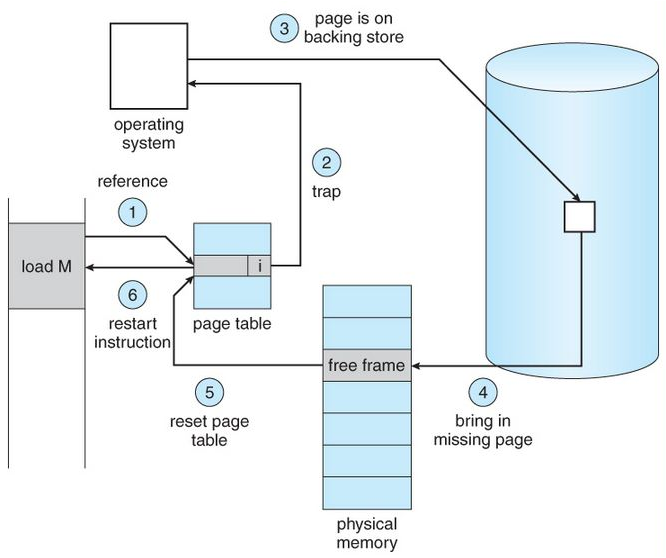
\includegraphics[width=1\linewidth]{content/OS_Internals/img/bnetg.png}
    \captionof{figure}{Page fault}

  \end{minipage}
\end{minipage}


\subsection{Costo di un page fault}
Supponiamo un tasso di page fault 0 < p < 1; se p = 0 nessun page fault, se p = 1 ogni riferimento è un fault.

Tempo di accesso effettivo:

\begin{itemize}
  \centering
  \item[] EAT = (1 - p) x accesso in memoria + p (overhead page fault + swap page out + swap page in)
\end{itemize}

Tempo di accesso in memoria = 200 nanosecondi; tempo medio di gestione del page fault = 8 millisecondi; un accesso su 1.000 causa un page fault. Sembra un numero piccolo, ma non lo è!

\paragraph{}
Ipotizzando un tempo di accesso RAM = 200 nanosecondi, tempo medio di gestione del page fault = 8 millisecondi:

\begin{itemize}
  \centering
  \item[] EAT = (1 - p)200 + p (8 millisecondi) = 200 + p7.999.800
\end{itemize}

Se un accesso su 1.000 causa un page fault, allora EAT = 8,2 microsecondi.

Questo è un rallentamento di un fattore 8,2 / 0,2 = 41!! Non è per niente buono!
Peggio della TLB.

\paragraph{}
Questa è probabilmente la fonte principale di rallentamenti quando si elabora qualcosa.

\section{Aspetti nel richiedere paging}



Caso estremo - avviare un processo senza pagine in memoria. La prima fatch genererà subito un
page falut.


Il sistema operativo imposta il puntatore dell'istruzione alla prima istruzione del processo,
che non è residente in memoria, causando un page fault. E questo accade per ogni pagina del
processo al primo accesso, il che è noto come \textbf{pure demand paging}.

In realtà, un certa istruzione potrebbe accedere a più pagine $\to$ più page fault.
Considera il fetch e decode di un'istruzione che aggiunge 2 numeri dalla memoria e
memorizza il risultato nuovamente in memoria. Il dolore (pain) è diminuito a causa della
località di riferimento, Locality of reference.


Il supporto hardware necessario per il demand paging include:
\begin{itemize}
  \item[] Tabella delle pagine con bit valido/invalido
  \item[] Memoria secondaria (dispositivo di swap con spazio di swap)
  \item[] Riavvio dell'istruzione
\end{itemize}

\section{Riavvio dell'Istruzione}

Considera un istruzione che può accedere a più locazioni, indirizzi, di memoria.
La sorgente e la destinzione in alcuni caso possono sovrapporsi.

\begin{itemize}
  \item Back move
  \item Auto incremento/decremento della locazione
  \item Riavviare l'intera operazione? Cosa succede se l'istruzione destinataria è overlapped?
\end{itemize}

\section{Strategia di sostituzione delle pagine}

Quando si verifica un page fault, il sistema operativo deve portare la
pagina desiderata dalla memoria secondaria nella memoria principale.

La maggior parte dei sistemi operativi mantiene una lista di frame liberi -- un pool
di frame liberi per soddisfare tali richieste.

Il puntatore è inserito proprio nel frame e quando un frame è libero utilizzala per non
allocare un'altra struttura per contenere la lista di frame.


\begin{figure}[htbp]
  \centering
  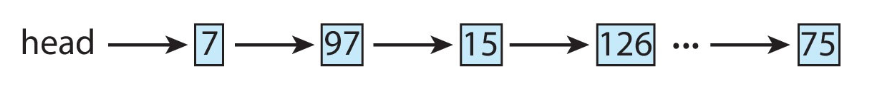
\includegraphics[width=0.4\linewidth]{content/OS_Internals/img/rhsbgfw.png}
\end{figure}

I sistemi operativi tipicamente allocano i frame liberi tramite una tecnica nota
come zero-fill-on-demand -- il contenuto dei frame viene azzerato prima di essere allocato.
All'avvio del sistema, tutta la memoria disponibile viene inserita nella lista dei frame liberi.

\subsection{Passi nel richiedere Paging - Caso Peggiore}

\begin{enumerate}
  \item Trap all'operating system con conseguente context switch
  \item Salva i registri utente e lo stato del processo
  \item Determina che l'interruzione è stata causata da un page fault
  \item Controlla che il riferimento alla pagina sia legale, altrimenti abort, e determina la posizione della pagina sul disco
  \item Emetti una lettura dal disco a un frame libero:
        \begin{itemize}
          \item[] Attendi in una coda per questo dispositivo fino a quando la richiesta di lettura non viene soddisfatta
          \item[] Attendi il tempo di seek e/o latenza del dispositivo
          \item[] Inizia il trasferimento della pagina a un frame libero
        \end{itemize}
  \item Mentre aspetti, assegna la CPU a qualche altro utente
  \item Ricevi un'interruzione dal sottosistema I/O del disco (I/O completato)
  \item Salva i registri e lo stato del processo per l'altro utente
  \item Determina che l'interruzione è stata causata dal disco
  \item Correggi la tabella delle pagine e altre tabelle per mostrare che la pagina è ora in memoria
  \item Attendi che la CPU venga assegnata a questo processo di nuovo
  \item Ripristina i registri utente, lo stato del processo e la nuova tabella delle pagine, quindi riprendi l'istruzione interrotta
\end{enumerate}

\subsection{Ottimizzazioni della Paginazione su Richiesta}

Lo swap space è più veloce dell'I/O del file system anche se sullo stesso dispositivo; lo swap viene allocato in blocchi più grandi, richiedendo meno gestione rispetto al file system; copia l'intera immagine del processo nello spazio di swap (backing store) al momento del caricamento del processo, quindi pagina dentro e fuori dallo spazio di swap; usato in BSD Unix più vecchio; demand page dal programma binario su disco, ma scarta piuttosto che paginare quando si libera un frame; usato in Solaris e BSD attuale; è ancora necessario scrivere nello spazio di swap per le pagine non associate a un file (come stack e heap) - memoria anonima - o per le pagine modificate in memoria ma non ancora scritte indietro al file system; i sistemi mobili tipicamente non supportano lo swapping, invece demand page dal file system e reclamano le pagine di sola lettura (come il codice).

\subsection{Copia su Scrittura (Copy-on-Write)}
% Più efficiente perché è già in memoria. Tutto va bene se leggono e possono rimanere
% condivise, ma quando inziano a modificarle devono essere copiate.
% Perrmette di efficientare l'utilizzo di memoria, si copia solo quelle che vengono modificate.

Copy-on-Write (COW) consente sia al processo padre che a quello figlio di condividere inizialmente le stesse pagine in memoria. Se uno dei processi modifica una pagina condivisa, solo allora la pagina viene copiata. COW consente una creazione di processi più efficiente poiché vengono copiate solo le pagine modificate. In generale, le pagine libere vengono allocate da un pool di pagine zero-fill-on-demand. Il pool dovrebbe sempre avere frame liberi per un'esecuzione rapida del demand page; non si vuole dover liberare un frame oltre ad altre elaborazioni su un page fault. Perché azzerare una pagina prima di allocarla? La variazione vfork() della system call fork() sospende il processo padre e il figlio utilizza lo spazio degli indirizzi copy-on-write del padre. Progettato per far sì che il figlio chiami exec(), molto efficiente.

\begin{center}
  \centering
  \begin{minipage}{0.85\linewidth}
    \begin{minipage}{0.47\linewidth}
      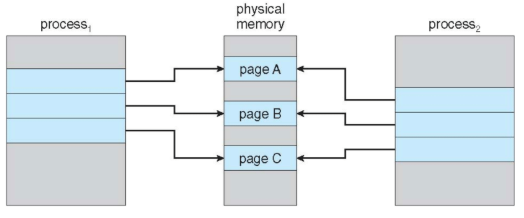
\includegraphics[width=1\linewidth]{images/OS_internals/Main-memory/MM-esempio9.png}


    \end{minipage}% <-- IMPORTANTE: il simbolo % qui evita spazi bianchi extra
    \hfill
    \begin{minipage}{0.47\linewidth}
      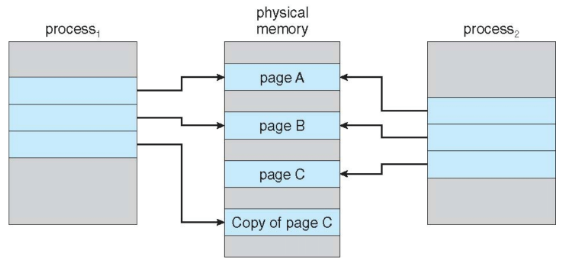
\includegraphics[width=1\linewidth]{images/OS_internals/Main-memory/MM-esempio10.png}

    \end{minipage}
  \end{minipage}
\end{center}


\subsection{Cosa succede se non ci sono frame liberi?}

\begin{center}
  \centering
  \begin{minipage}{\linewidth}
    % Primo blocco: 50% dello spazio per il codice
    \begin{minipage}{0.6\linewidth}

      Come per gli algoritmi di scheduling, possiamo implementare la soluzione più semplice usando la casualità: prendere un frame in memoria, metterlo nell'HD e caricare la pagina necessaria nella RAM; questa soluzione non è ottimale!

      Questa tecnica, indipendentemente dall'algoritmo, si chiama \textbf{sostituzione di pagina} - trovare una pagina in memoria non realmente in uso, rimuoverla e caricare la pagina necessaria.

      \paragraph{}
      Si previene la sovra-allocazione della memoria modificando la routine di gestione dei page fault in modo da includere la sostituzione delle pagine.

      Possiamo farlo usando il \textbf{bit di modifica (dirty bit)} per ridurre l'overhead dei trasferimenti di pagina - solo le pagine modificate vengono scritte su disco.

      Se il dirty bit è impostato significa che il valore nella RAM è cambiato e prima di caricare la nuova pagina devo scrivere il valore nell'HD.

      La sostituzione delle pagine completa la separazione tra memoria logica e
      fisica - una grande memoria virtuale può essere fornita con una memoria
      fisica più piccola.

      \paragraph{}

      Questo processo significa accedere all'HD \textbf{due volte}.

    \end{minipage}% <-- IMPORTANTE: il simbolo % qui evita spazi bianchi extra
    \hfill
    \begin{minipage}{0.37\linewidth}
      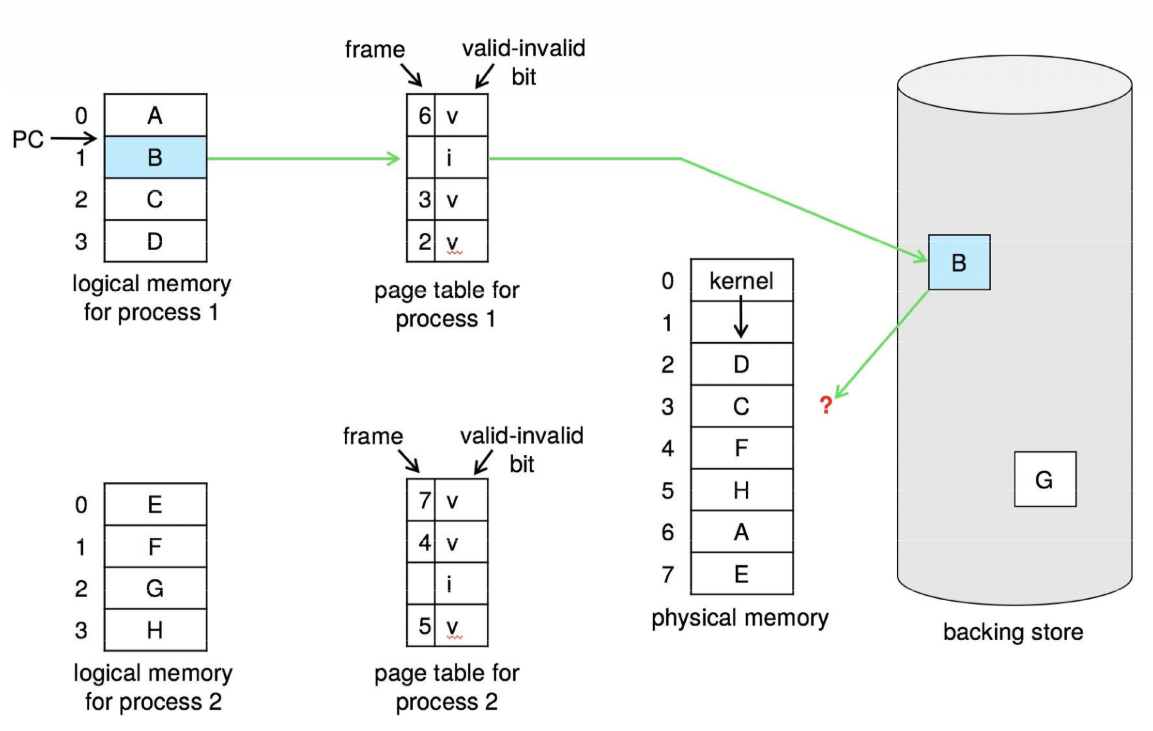
\includegraphics[width=1\linewidth]{content/OS_Internals/img/sdfbgv.png}

    \end{minipage}
  \end{minipage}
\end{center}


\subsection{Sostituzione di pagina di base}


\begin{minipage}{1\linewidth}
  % Primo blocco: 50% dello spazio per il codice
  \begin{minipage}{0.6\linewidth}
    \begin{enumerate}
      \item Trovare la posizione della pagina desiderata su disco
      \item Trovare un frame libero:
            \begin{itemize}
              \item[] Se c'è un frame libero, usarlo
              \item[] Se non c'è un frame libero, usare un algoritmo di sostituzione delle pagine per selezionare un frame vittima
              \item[] Scrivere il frame vittima su disco se è sporco (= modificato mentre era in RAM)
            \end{itemize}
      \item Caricare la pagina desiderata nel frame (appena) libero; aggiornare le tabelle delle pagine e dei frame
      \item Continuare il processo riavviando l'istruzione che ha causato il trap
    \end{enumerate}
  \end{minipage}% <-- IMPORTANTE: il simbolo % qui evita spazi bianchi extra
  \hfill
  \begin{minipage}{0.36\linewidth}
    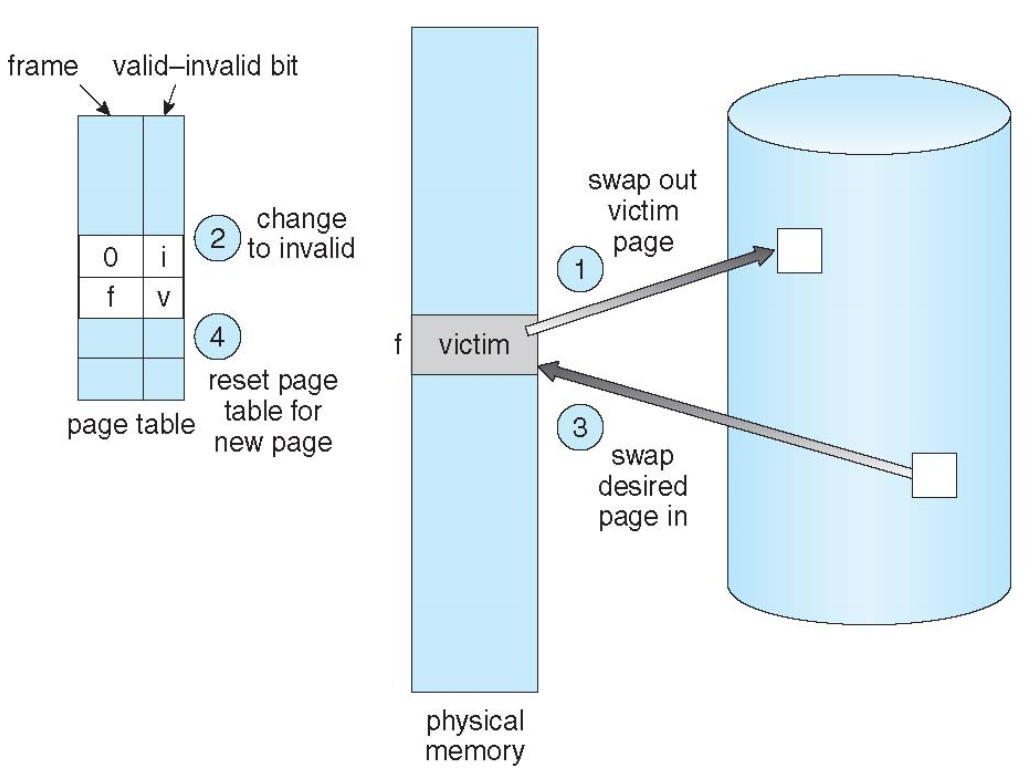
\includegraphics[width=1\linewidth]{content/OS_Internals/img/mghj.png}


  \end{minipage}
\end{minipage}




% inizio 30/03/2026

\section{Algoritmi di sostituzione di pagine e frame}


\begin{minipage}{1\linewidth}
  % Primo blocco: 50% dello spazio per il codice
  \begin{minipage}{0.6\linewidth}

    L'algoritmo di allocazione dei frame determina:

    \begin{enumerate}
      \item Quanti frame assegnare a ciascun processo
      \item Quali frame sostituire; idealmente sostituisco solo la pagina che non mi servirà presto (ma non conosco il futuro)
    \end{enumerate}


    Algoritmo di sostituzione delle pagine:

    \begin{itemize}
      \item[] Si vuole che il tasso di page fault più basso sia al primo accesso che ai successivi
    \end{itemize}

  \end{minipage}% <-- IMPORTANTE: il simbolo % qui evita spazi bianchi extra
  \hfill
  \begin{minipage}{0.36\linewidth}
    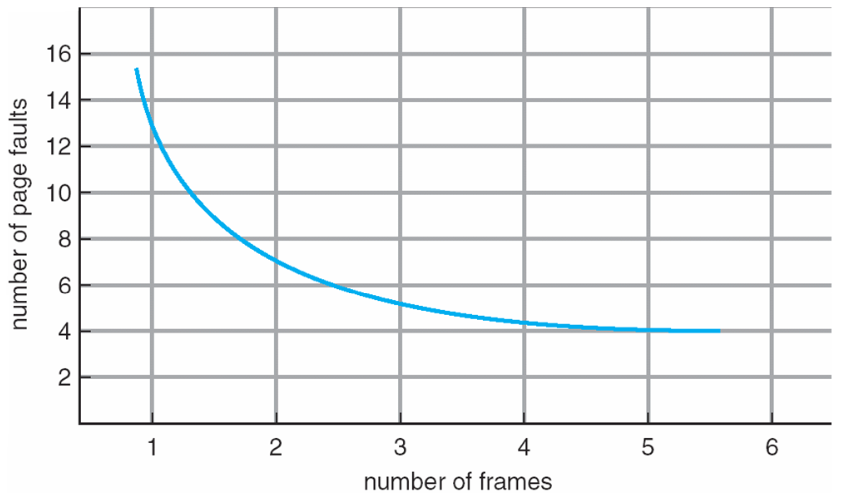
\includegraphics[width=1\linewidth]{content/OS_Internals/img/ahet.png}

  \end{minipage}
\end{minipage}

\vspace{0.5cm}

In questa immagine si può vedere che più frame slot sono associati a ogni processo, minore è la probabilità di avere page fault.

\subsection{Frequenza di Page Fault - probability empirica}



\begin{equation*}
  f(A, m) = \sum_{\forall w} p(w) \frac{F(A, w, m)}{len(w)}
\end{equation*}

dove

\begin{flushleft}
  \begin{minipage}{0.65\linewidth}
    \raggedright
    \begin{itemize}
      \setlength{\itemsep}{6pt}
      \item \textbf{A} un algoritmo di sostituzione delle pagine in valutazione
      \item \textbf{w} una data stringa di riferimento
      \item \textbf{p(w)} probabilità di riferimento alla stringa \textbf{w}
      \item \textbf{len(w)} lunghezza della stringa \textbf{w}
      \item \textbf{m} numero di page frame liberi
      \item \textbf{F(A, w, m)} numero di page fault causati data una certa stringa di riferimento \textbf{w} usando l'algoritmo \textbf{A} sul sistema di un dato sistema con \textbf{m} page frame
    \end{itemize}
  \end{minipage}%
  \hfill
  \begin{minipage}{0.3\linewidth}
    \centering
    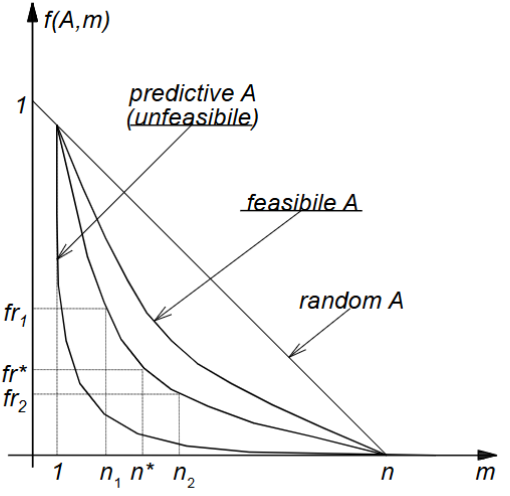
\includegraphics[width=\linewidth]{content/OS_Internals/images/2026-03-30-11-58-12.png}
  \end{minipage}
\end{flushleft}


Ci aspettiamo che un dato algoritmo casuale abbia una curva lineare decrescente.
Mentre il caso migliore, ovvero l'algoritmo che prevede il futuro, abbia una curva decrescente più ripida.


Quindi dato un algoritmo e il numero n di frame e troviamo la frequenza di page fault.

\subsection{Selezione delle vittime usando il modify bit}

\begin{center}
  \begin{minipage}{0.65\linewidth} % Ridotto leggermente per dare spazio alla tabella
    Quando si sceglie la vittima, la pagina da buttare fuori per far posto alla nuova,
    si deve guardare il \textit{reference bit} (se una pagina è stat usata nel passato recente) e il \textit{modify bit}
    (se è stata modificata) i quali indicano se la pagina è attiva o meno e possiamo
    utilizzare questa informazione per scegliere la vittima negli algoritmi di sostituzione delle pagine.

    \begin{tcolorbox}
      \textbf{Nota:} Il caso migliore è 00, il caso peggiore è 11.
    \end{tcolorbox}

  \end{minipage}%
  \hfill
  \begin{minipage}{0.3\linewidth} % Allargato per far stare il testo della tabella
    \centering
    \renewcommand{\arraystretch}{1.6}
    \small % Opzionale: rende la tabella leggermente più piccola per farla stare meglio
    \begin{tabular}{cc}
      \hline
      \textbf{Ref. bit} & \textbf{Mod. bit} \\
      \hline
      0                 & 0                 \\
      0                 & 1                 \\
      1                 & 0                 \\
      1                 & 1                 \\
      \hline
    \end{tabular}
  \end{minipage}
\end{center}


\subsection{Algoritmo FIFO}

Si assume che una pagina che è entrata in memoria prima delle altre
sia stata già utilizzata e l'algoritmo FIFO selezionerà quella pagina.

Stringa di riferimento: 7,0,1,2,0,3,0,4,2,3,0,3,0,3,2,1,2,0,1,7,0,1;

m = 3 frame, 3 pagine possono essere in memoria contemporaneamente per processo.
Dentro i frame troviamo il \textbf{residence set} di 3 pagine.

\begin{figure}[h!]
  \centering
  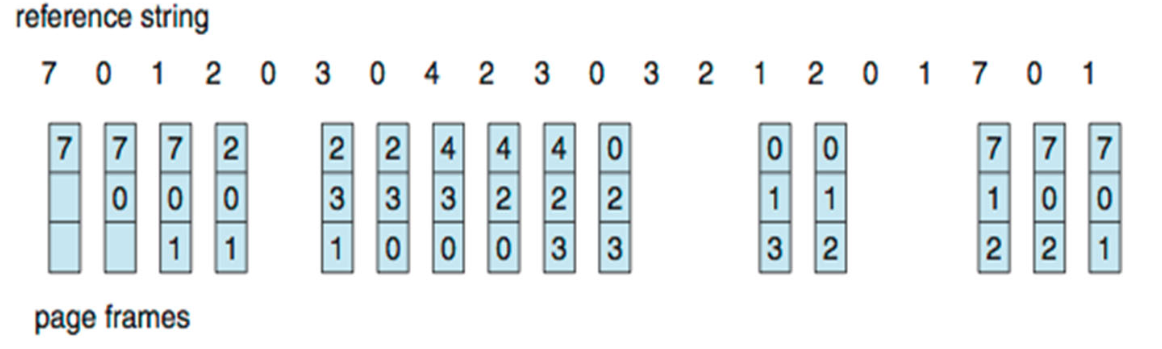
\includegraphics[width=0.5\linewidth]{content/OS_Internals/img/dgnf.png}
\end{figure}

Dopo i primi 3 page fault, dato il pure demand paging, dopo vi inizierà l'algoritmo di
sostituzione delle pagine.


\begin{center}
  \begin{minipage}{0.65\linewidth}
    Possiamo realizzare l'algoritmo: con una lista concatenata con inserimento in coda e rimozione in testa (illimitato);
    altrimenti con una coda circolare (limitato).
    In questo ultimo caso siamo davanti ad un FIFO circolare semplificato:
    inizialmente 2 puntatori per head e tail, una volta riempito tutto mi basta ricordare
    solo il puntatore a head e portarlo avanti.

    \paragraph{}
    Con questo metodo si hanno 15 page fault; si può fare meglio?
    FIFO veloce, $O(1)$, ma non è un buon algoritmo!

    \begin{tcolorbox}
      \textbf{Nota:} Non è sempre vero che, sullo specifico caso,
      aumentando il numero di frame si riduca il numero di page fault; questo
      fenomeno è noto come \textbf{anomalie di Belady}.
    \end{tcolorbox}



  \end{minipage}%
  \hfill
  \begin{minipage}{0.3\linewidth}
    \centering
    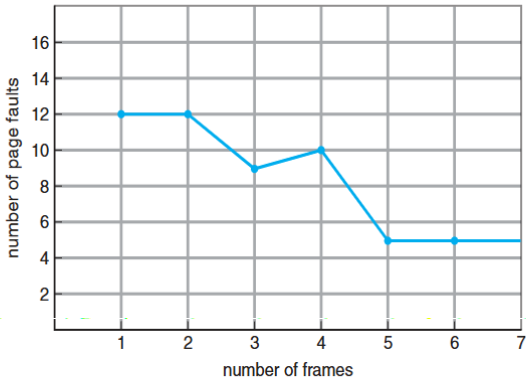
\includegraphics[width=\linewidth]{content/OS_Internals/images/2026-03-30-12-15-48.png}
  \end{minipage}
\end{center}


\subsection{Algoritmo ottimale}

L'algoritmo ottimale sceglie la pagina che non verrà utilizzata per il periodo più lungo nel futuroe questo
diminuisce, per questo specifico esempio, il numero di page fault a 9.


Ma come detto non possiamo prevedere il futuro; TUTTAVIA questa è
la soluzione ottimale e dunque possiamo utilizzarla per misurare le prestazioni
degli altri algoritmi.

\begin{figure}[h!]
  \centering
  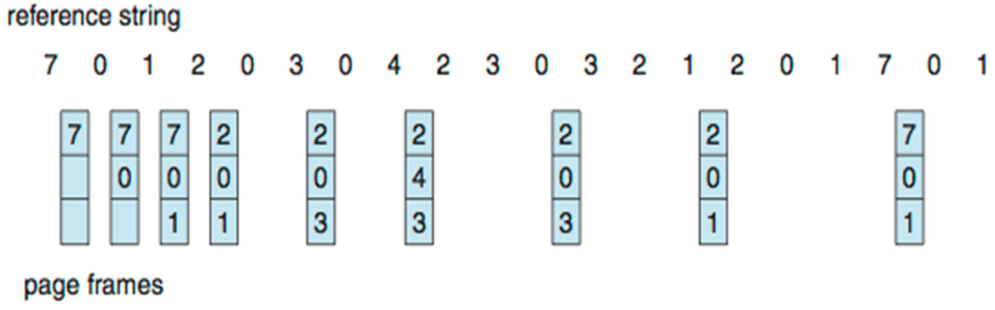
\includegraphics[width=0.5\linewidth]{content/OS_Internals/img/dng.png}
\end{figure}


\begin{tcolorbox}
  \textbf{Nota:} Anche in questo caso non eliminiamo completamente i page fault dato che i
  frame sono limitati.
\end{tcolorbox}


\subsection{Algoritmo LRU - Least Recently Used}

Abbiamo visto che il programma non può conoscere il futuro, ma possiamo usare la conoscenza del passato!

Sostituisce la pagina che non è stata utilizzata per il periodo di tempo più lungo; sfrutta il \textbf{principio di località temporale},
associando ad ogni pagina il tempo dell'ultimo utilizzo.

L'assunzione di questo algoritmo è che una pagina che è stata utilizzata poco nel passato sarà utilizzata poco anche nel futuro.

Associamo ad ogni pagina il numero di accessi alla pagina, ma di difficile da implementare senza
consumare memoria aggiuntiva e rallentare il sistema.
Inoltre dovrà essere implementata una ricerca lineare e suppone
che una pagina si mantenga traccia dell'accesso.

\begin{figure}[h!]
  \centering
  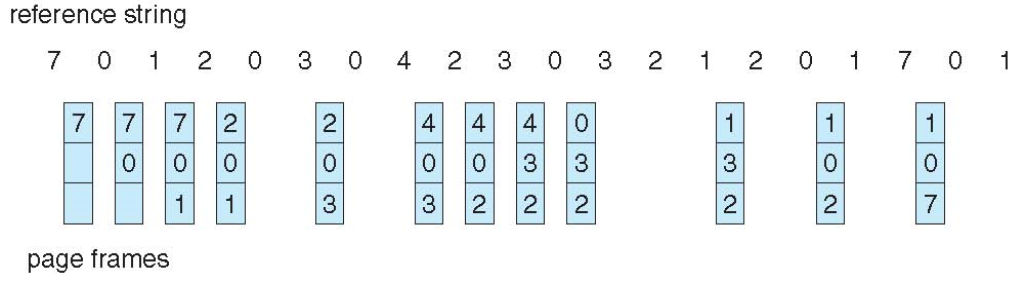
\includegraphics[width=0.5\linewidth]{content/OS_Internals/img/fdb.png}
\end{figure}

12 page fault - meglio di FIFO ma peggio di OPT; generalmente un buon algoritmo e ampiamente usato. Ma come si implementa?

\begin{figure}[h!]
  \centering
\end{figure}


\begin{center}
  \begin{minipage}{0.3\linewidth}
    \begin{equation*}
      f = \frac{10}{12} = 0.83\,\to\,83\%
    \end{equation*}
  \end{minipage}
  \hfill
  \begin{minipage}{0.65\linewidth}
    \centering
    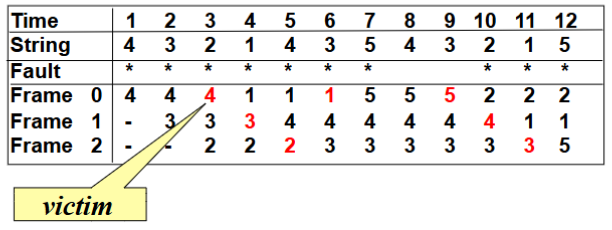
\includegraphics[width=0.7\linewidth]{content/OS_Internals/images/2026-03-30-12-25-13.png}

  \end{minipage}%
\end{center}


\paragraph{Implementazione con contatore: } Ogni voce di pagina ha un contatore;
ogni volta che la pagina viene referenziata, sia in lettura o scrittura, si copia il clock nel contatore, il tempo di accesso.
Quando una pagina deve essere sostituita, si cerca il contatore con il valore minore; è necessaria una ricerca nella tabella.

Il clock può essere nella TLB (costoso deve mantenere un int) che si aggiorna automaticamente oppure nella tabella delle pagine.
In ogni caso è di difficile implementazione.

% Scandisci tutti i contatori e trova il minimo. Deve essere hardware, ma costoso.

\begin{center}
  \begin{minipage}{0.65\linewidth}
    % Non ricordo il tempo ma cerco di fare una struttura dati ordinata, implementazione
    % con stack (non con push e pop) lista doppiamente concatenata.

    \paragraph{Implementazione con stack (lista concatenata): }Si mantiene uno stack
    di numeri di pagina in forma di lista doppiamente concatenata. Quando una pagina
    viene referenziata, viene spostata in cima. È necessario aggiornare 6 puntatori
    per ogni accesso alla pagina \footnote{Si deve rimuovere la pagina dalla lista e inserirla in cima e i riferimenti devono essere aggiornati}.


    % Tutte le pagine sono nella lista ordinate per tempo di accesso, la prima in testa,
    % quando accedi una pagina estrai (O(1)) e la metti in cima quadno ha un riferimento,
    % aggiornamento di 6 puntatori da aggiornare quindi scritture e letture. Quindi costa
    % per ogni accesso alla pagina.

    Estrazione $O(1)$ ma inserimento costoso.

    % Ma ogni aggiornamento è più costoso e non è necessaria una ricerca per la sostituzione.

    \paragraph{}
    LRU e OPT sono casi di algoritmi a stack che non hanno l'anomalia di Belady. Si usa uno stack per registrare i riferimenti alle pagine più recenti.

  \end{minipage}%
  \hfill
  \begin{minipage}{0.3\linewidth}
    \centering
    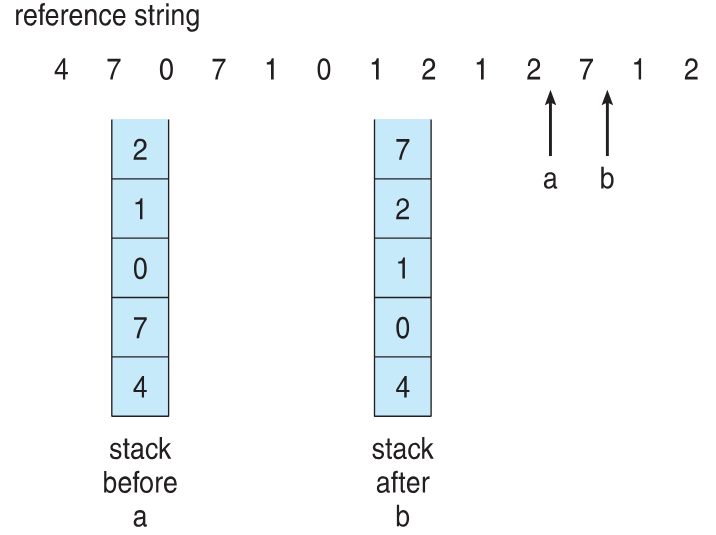
\includegraphics[width=\linewidth]{content/OS_Internals/img/sd.png}
  \end{minipage}
\end{center}


\subsection{Algoritmi LRU approssimati}

LRU richiede hardware speciale ed è comunque lento e costoso in termini di memoria (4 byte per ogni voce).
% Credo che Abbiamo una distinzione binaria tra vittime e no vittime.

Possiamo semplificare LRU utilizzando un solo bit: il \textbf{bit di riferimento}.
Inizialmente ad ogni pagina viene associato il bit con valore 0; quando
la pagina viene referenziata il bit viene impostato a 1. Se il SO
necessita di memoria per un processo, può sostituire qualsiasi pagina
con il bit a 0, se ne esiste una.


Prima o poi tutte le pagine avranno il bit di riferimento a 1, perciò
dobbiamo trovare un modo per azzerarlo.

% Prima o poi ci saranno tutte le pagine con bit di riferimento a 1,
% ci sarà un momento in cui verranno azzerati tutti i bit di riferimento a 0.



\begin{flushleft}
  \begin{minipage}{0.65\linewidth}
    \raggedright
    \subsubsection{Algoritmo second-chance: } Generalmente FIFO, più il bit di riferimento fornito dall'hardware con sostituzione \textbf{Clock} - buffer circolare.
    Nel caso peggiore, l'algoritmo scorre l'intera lista.
    Se la pagina da sostituire ha:

    \begin{itemize}
      \item Bit di riferimento = 0 $\to$ sostituirla
      \item Bit di riferimento = 1 allora:
            \begin{itemize}
              \item[] impostare il bit di riferimento a 0, lasciare la pagina in memoria, così che al secondo passaggio la trovo a 0
              \item[] sostituire la pagina successiva, con le stesse regole
            \end{itemize}
    \end{itemize}

    Messo ad 1 dalla TLB in hw, messo a zero dal software dato che si
    ha molto tempo a disposizione causa il page fault.
  \end{minipage}%
  \hfill
  \begin{minipage}{0.3\linewidth}
    \centering
    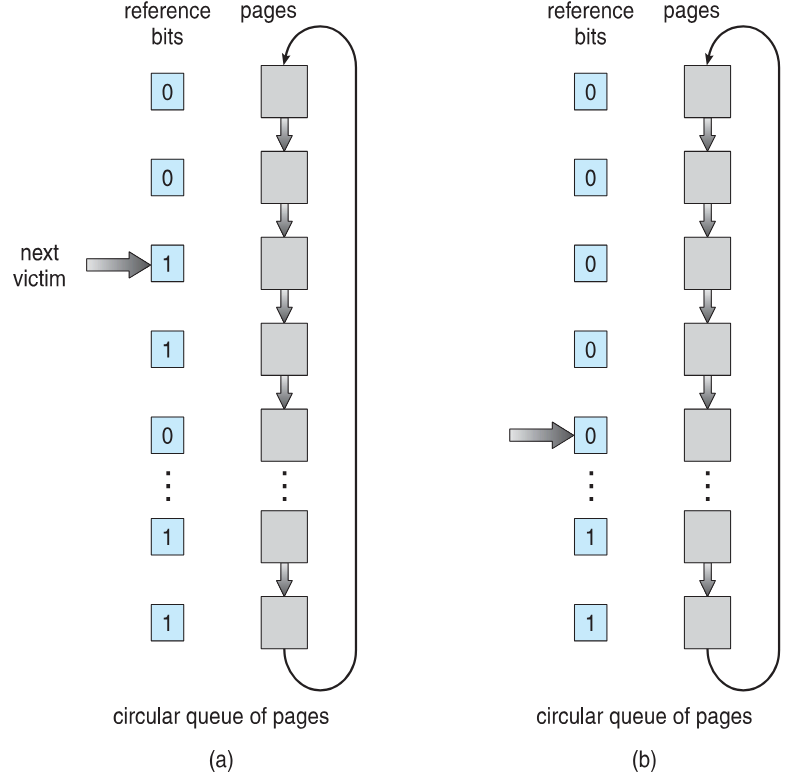
\includegraphics[width=\linewidth]{content/OS_Internals/img/jnyfg.png}
  \end{minipage}
\end{flushleft}


\subsubsection{Miglioramento dell'Algoritmo della Seconda Chance}

% Preferisco che il modify bit sia 0, significo che sia in memoria
% sia sul disco le pagine sono uguali così da minimizzare il tempo
% per la gestione dei page fault.

Possiamo migliorare l'algoritmo usando il bit di riferimento e il bit di modifica (se disponibile) in concerto. Prendiamo la coppia ordinata (riferimento, modifica):
\begin{itemize}
  \item (0, 0) né recentemente usata né modificata --- la migliore pagina da sostituire, minimizza il tempo di gestione del page fault
  \item (0, 1) non recentemente usata ma modificata --- non così buona, deve essere scritta prima della sostituzione
  \item (1, 0) recentemente usata ma pulita --- probabilmente sarà usata di nuovo presto
  \item (1, 1) recentemente usata e modificata --- probabilmente sarà usata di nuovo presto e deve essere scritta prima della sostituzione
\end{itemize}
Quando viene chiamata la sostituzione di pagina, si utilizza lo schema clock ma si usano le quattro classi per sostituire la pagina nella classe non vuota più bassa. Potrebbe essere necessario cercare più volte nella coda circolare.


Prima di cercare 0,1 devo rifare tutto il giro, e via così fino a 1,1 quindi al massimo
faccio almeno 3 giri. Ovviamente si può fare in un giro solo ma devo
occupare memoria.


Questo si basa sempre dell'LRU, che misura un'inattività della pagina.



\subsection{Algoritmi basati sul conteggio}
Si mantiene un contatore del numero di riferimenti effettuati a ogni pagina; non comune.

\begin{tcolorbox}
  \textbf{Nota:}  Anche qui prima o poi si deve azzerare tutti i contatori.
\end{tcolorbox}


\subsubsection{Algoritmo LFU (Least Frequently Used):}

\begin{itemize}
  \item Sostituisce la pagina con il contatore più basso
  \item Problema: può capitare che venga sempre sostituita la pagina appena inserita dato che hanno il contatore impostato a 1
\end{itemize}


\subsubsection{Algoritmo MFU (Most Frequently Used):}

Si basa sull'argomento che la pagina con il contatore più basso è stata probabilmente appena caricata e non è ancora stata utilizzata


\subsection{Page-Buffering Algorithms}

Prendiamo un pool di frame liberi, sempre disponibile quando necessario, non trovato al momento del page fault. Leggiamo la pagina in un frame libero e selezioniamo una vittima da espellere e aggiungiamo al pool dei frame liberi. Quando è conveniente, espelliamo la vittima, possibilmente tenendo una lista di pagine modificate. Quando lo storage secondario è altrimenti inattivo, scriviamo le pagine lì e impostiamo a non sporco. Possibilmente, manteniamo intatti i contenuti del frame libero e annotiamo cosa c'è dentro; se viene referenziato di nuovo prima di essere riutilizzato, non c'è bisogno di caricare nuovamente i contenuti da disco. Generalmente utile per ridurre la penalità se viene selezionato il frame vittima sbagliato.


Soluzioni aggiuntive rispetto ai precedenti, vogliamo ridurre il \textbf{tempo} di gestione del page fault.

Quando cerco un frame libero lo ottendo, dato che mi sono tenuto qualche frame libero.
Quando si verifica un page fault cerco una vittima, la quale verrà espulsa solo quando è conveniente.

Le vittime sono lasciate ancora con il contenuto e nel caso se fai riferimento ad una
vittima prima che venga espulsa, non c'è bisogno di caricarla da disco.


Mantengo le vittime fino a che non ho proprio bisogno di liberare frame,
nel mentre le mantengo in memoria anche se sono segnate come vittima.

\begin{tcolorbox}
  \textbf{Nota:} Immagina il cestino di un sistema operativo.
\end{tcolorbox}


\subsection{Applicazioni e Sostituzione delle Pagine}

Tutti questi algoritmi di sostituzione delle pagine sono basati su ipotesi e non possono prevedere con precisione il futuro accesso alle pagine. Tuttavia, alcune applicazioni, come i database, hanno una migliore conoscenza dei loro modelli di accesso alla memoria e possono utilizzare questa conoscenza per ottimizzare le prestazioni. Le applicazioni che richiedono molta memoria possono causare un doppio buffering, in cui il sistema operativo mantiene una copia della pagina in memoria come buffer I/O, mentre l'applicazione mantiene la pagina in memoria per il proprio lavoro. In questi casi, il sistema operativo può fornire un accesso diretto al disco, bypassando il buffering e altre funzionalità del sistema operativo, consentendo all'applicazione di gestire direttamente l'I/O del disco.


\section{Allocazione dei frame ai processi}

Quanto deve valere m e come facciamo a deciderlo?

Ogni processo necessita di un numero minimo di frame; il massimo è ovviamente il numero totale di frame nel sistema.

Due principali schemi di allocazione: \textbf{allocazione fissa} e \textbf{allocazione a priorità}, oltre a molte varianti.

\subsection{Allocazione fissa}
L'allocazione data ad un dato processo è fissa


\paragraph{Allocazione eguale} se ci sono 100 frame (dopo aver allocato i frame per il SO) e 5 processi, si assegnano 20 frame a ciascun processo. Si mantiene anche una parte come pool di frame liberi.

\paragraph{Allocazione proporzionale}

Si alloca in base alla dimensione del processo; dinamica in funzione del grado di multiprogrammazione, le dimensioni dei processi cambiano.

\begin{itemize}
  \item $s_i$ = dimensione del processo $p_i$ in pagine
  \item $S = \sum{s_i}$
  \item m = numero totale di frame disponibili
  \item $a_i$ = numero di frame allocati a $p_i$ = $\frac{s_i}{S} \cdot m$
\end{itemize}

\begin{equation*}
  m = 64 \quad s_1 = 10 \quad s_2 = 127 \quad a_1 = \frac{10}{137} \cdot 62 \approx 4 \quad a_2 = \frac{127}{137} \cdot 62 \approx 57
\end{equation*}

\paragraph{}


In entrambi i tipi di allocazione non è possibile tener conto dei task ad alta/bassa priorità;
idealmente si vorrebbe che quelli ad alta priorità terminassero prima, assegnando loro più
memoria/CPU.

\subsection{Allocazione globale vs. locale}

\textbf{Sostituzione globale} - il processo seleziona un frame di sostituzione dall'insieme di tutti i frame.

\begin{itemize}
  \item un processo può sottrarre un frame a un altro
  \item il tempo di esecuzione del processo può variare notevolmente dato che dipende da ciò che stanno facendo gli altri processi
  \item throughput maggiore, quindi più comune
\end{itemize}

\textbf{Sostituzione locale} - ogni processo seleziona solo dal proprio insieme di
frame allocati

\begin{itemize}
  \item Prestazioni per processo più consistenti
  \item possibile sottoutilizzo della memoria
  \item Quindi, throughput minore
\end{itemize}

\subsection{Recupero delle pagine}

\begin{center}
  \centering
  \begin{minipage}{1\linewidth}
    % Primo blocco: 50% dello spazio per il codice
    \begin{minipage}{0.65\linewidth}

      Una strategia per implementare la politica di sostituzione globale è: tutte le richieste di memoria vengono soddisfatte dalla lista dei frame liberi, invece di aspettare che la lista scenda a zero prima di iniziare a selezionare le pagine da sostituire. Il recupero delle pagine viene attivato dal kernel quando la lista scende sotto una certa soglia.

      \paragraph{}
      Il processo kernel che lo gestisce è chiamato \textbf{reaper}.

      Questa strategia cerca di garantire che ci sia sempre sufficiente memoria libera per soddisfare le nuove richieste, ovvero che la lista dei frame liberi non si svuoti mai.

    \end{minipage}% <-- IMPORTANTE: il simbolo % qui evita spazi bianchi extra
    \hfill
    \begin{minipage}{0.3\linewidth}
      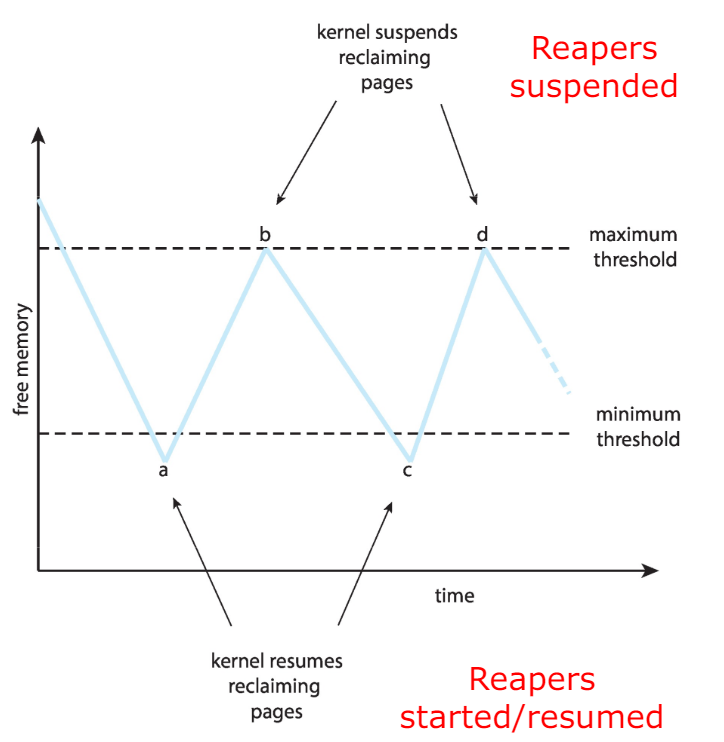
\includegraphics[width=0.7\linewidth]{content/OS_Internals/img/andg.png}
      \captionof{figure}{Esempio di recupero delle pagine}

    \end{minipage}
  \end{minipage}
\end{center}

\subsection{Non-Uniform Memory Access}



\begin{center}
  \centering
  \begin{minipage}{1\linewidth}
    % Primo blocco: 50% dello spazio per il codice
    \begin{minipage}{0.65\linewidth}

      Fino ad ora tutta la memoria è stata considerata uguale, ma molti sistemi sono NUMA (Non-Uniform Memory Access) - la velocità di accesso alla memoria varia. Considera le schede di sistema contenenti CPU e memoria, interconnesse tramite un bus di sistema - architettura di multiprocessing NUMA.\newline

      La memoria condivisa fa sì che tutti i core rallentano e relativi problemi di
      consistenza.
      Sarebbe auspicabile che un processo che è stato allocato alla CPU1 usa la memoria
      memoria locale alla CPU1. Tutto questo diventa ancora più complicato quando
      un processo viene migrato da una CPU a un'altra.
    \end{minipage}% <-- IMPORTANTE: il simbolo % qui evita spazi bianchi extra
    \hfill
    \begin{minipage}{0.3\linewidth}
      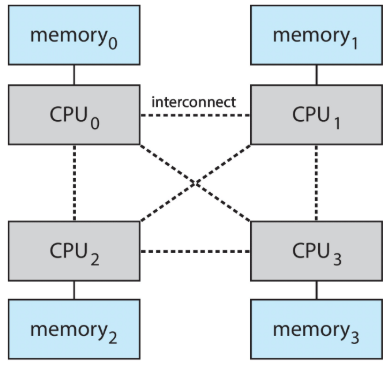
\includegraphics[width=0.7\linewidth]{images/OS_internals/Main-memory/MM-esempio11.png}

    \end{minipage}
  \end{minipage}
\end{center}

L'ottima prestazione deriva dall'allocare la memoria "vicino" alla CPU su cui è programmato il thread e modificare lo scheduler per programmare il thread sulla stessa scheda di sistema quando possibile. Soluzione adottata da Solaris creando lgroups, una struttura per tracciare i gruppi a bassa latenza CPU/memoria, usata dallo scheduler e dal pager. Quando possibile, schedula tutti i thread di un processo e allocare tutta la memoria per quel processo all'interno dell'lgroup.


In un multicore lo sheduler cerca di preferire la stessa CPU per un dato processo e
idem per l'allocazione della memoria.

\subsection{Thrashing}

\begin{center}
  \centering
  \begin{minipage}{1\linewidth}
    % Primo blocco: 50% dello spazio per il codice
    \begin{minipage}{0.65\linewidth}

      \textbf{Thrashing} - un processo è occupato a scambiare continuamente pagine in entrata e in uscita.
      \paragraph{}

      Se un processo non ha un numero "sufficiente" di pagine, il tasso di page fault è molto
      alto: \textbf{page fault} per ottenere la pagina, \textbf{sostituzione} del frame esistente, ma rapidamente si ha bisogno di nuovo del \textbf{frame sostituito}.

    \end{minipage}% <-- IMPORTANTE: il simbolo % qui evita spazi bianchi extra
    \hfill
    \begin{minipage}{0.3\linewidth}
      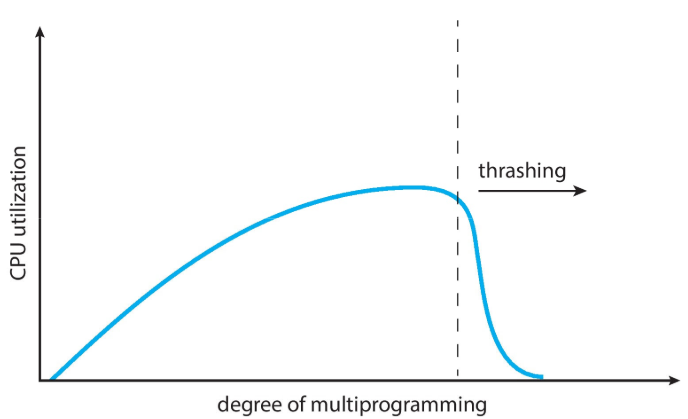
\includegraphics[width=1\linewidth]{content/OS_Internals/img/SDBF.png}

    \end{minipage}
  \end{minipage}
\end{center}
Tutti questi cicli portano a:

\begin{itemize}
  \item Basso utilizzo della CPU
  \item Il sistema operativo pensa di dover aumentare il grado di multiprogrammazione
  \item Un altro processo viene aggiunto al sistema
\end{itemize}

\subsection{Paging su richiesta e thrashing}

Vorrei che tutte le località a cui accedo siano in memoria.

Perché il demand paging funziona? Modello di località degli accessi:
\begin{itemize}
  \item[] Il processo migra da una località all'altra
  \item[] Le località possono sovrapporsi
\end{itemize}
Perché si verifica il thrashing? La somma delle dimensioni delle località è maggiore della dimensione totale della memoria.
Limitare gli effetti usando la sostituzione di pagina locale o a priorità.

\subsection{Working-Set Model}

Chiamiamo Working-Set le pagine su cui sta lavorando un processo. Come lo definiamo?
Le pagine su cui un processo sta lavorando cambia nel tempo, bisogna definire una
finestra di lavoro, $\Delta$, l'intervallo a cui faccio riferiento e.g. 10 000.

$\Delta$ è la finestra di lavoro, un numero fisso di riferimenti.
$WSS_i$ (Working Set Size) è il working set del processo $P_i$ , ovvero il numero totale di pagine referenziate nelle più recenti $\Delta$ istruzioni. D è la somma di tutti i $WSS_i$ , ovvero il numero totale di frame richiesti da tutti i processi.

\begin{itemize}
  \item se $Delta$ è troppo piccolo, non coprirà l'intera località. Fotografo un passato troppo recente e nel futuro probabilmente avrò bisogno di altre pagine che non sono nel working set. (Eg $Delta = 1$ la prossima volta faccio sicuramente page fault)
  \item se $Delta$ è troppo grande, coprirà diverse località.
  \item se $Delta = \infty$, coprirà l'intero programma. Tutto quello che ho usato nel passato lo considero parte del working e gli unici page fault sono solo le pagine a cui NON ho mai fatto acceso. Impossibile perché la memoria è finita.
\end{itemize}

Se D > m $\implies$ thrashing. Policy se D > m, allora sospendi o swap out uno dei processi.

\begin{figure}[h!]
  \centering
  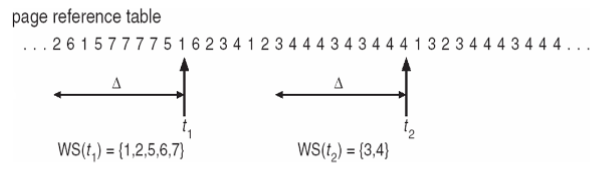
\includegraphics[width=0.5\linewidth]{content/OS_Internals/images/2026-03-30-14-03-18.png}
\end{figure}

Più il programma è locale più richiede pochi frame, migliorando la gestione della memoria.
Permette dinamicità globale tra i vari processi.

Caso ideale avere tutto il Working Set in memoria, e mi va meglio se è piccolo (WSS i piccolo).

\subsection{Tenere traccia del Working Set}

Essendo una slinding window, rischio di perdermi l'ultimo riferimento.
Prima attivo il page falut solo quando faccio riferimento ad una pagina ora invece
devo buttare via pagine (page out) quando faccio riferimento solo alle stesse pagine perché
il progamma è molto locale.

A rigore dovrei ricordami il periodo dell'ultimo accesso, simile a LRU.

Approssimativamente con un timer a intervalli + un bit di riferimento. Esempio: $\Delta = 10.000$ ; l'interruzione del timer avviene ogni $5000$ unità di tempo; mantenere in memoria 2 bit per ogni pagina; ogni volta che il timer interrompe, copiare e impostare i valori di tutti i bit di riferimento a 0; se uno dei bit in memoria $= 1 \implies$ pagina nel working set. Perché non è completamente accurato? Miglioramento $= 10$ bit e interruzione ogni $1000$ unità di tempo.


Approssimiamo l'intervallo e il working set reale sarà più grande, riallineandolo
solo ogni tanto.

I due bit sono \textbf{Reference bit} e \textbf{Reference bit precedente}.

Se ho una pagine ha il bit di riferimento a 1 allora ci ho fatto riferimento.
Uno fotografa i 5000 istanti prima e l'altro fotografa i 5000 istanti prima di quello.

Se allo scatto del timer, allino esattamente al working set altrimenti tra 10k e 15k dato che interrompo ogni $5000$ unità di tempo.

Ogni 5 istanti prima di riazzerare guardo tutte le pagine:
guardo i 2 bit: butto via le pagine con 00 le altre le tengo.
mentre facccio il giro, tutti i reference bit (gli ultimi) vengono azzerati e il loro
valore viene copiato nel bit che contieneva il reference bit precedente.



\paragraph{Working set}: cerchiamo di tenere traccia delle pagine in cui sto lavorando e solo ed almeno queste
le tengo in memoria. Utilizziamo un approssimazione, rispetto al cambiamneto di tutti i riferimenti,
di 5000 di instanti di tempo, sovapprossimando del 50\% (15000) instanti rispetto al teorico 10k.


\paragraph{Idea -} usare il tempo per dimensionare le pagine di lavoro, si può utilizzare la
frequenza rispetto al tempo



\subsection{Frequenza dei page fault}

Invece di rendere dimamica la sliding window, guardiamo l'effetto che otteniamo allocando
più o meno frame.


\begin{flushleft}
  \begin{minipage}{0.65\linewidth}
    \raggedright
    Si stabilisce un tasso di page fault (PFF) "accettabile" e si usa la politica di sostituzione locale.
    \begin{itemize}
      \item[-] Se il tasso effettivo è troppo basso, il processo perde un frame
      \item[-] Se il tasso effettivo è troppo alto, il processo guadagna un frame
    \end{itemize}

    Troviamo 2 soglie per evitare oscillazioni.
    Aumentando il numero di frame, m, si abbassa il tasso di page fault.

  \end{minipage}%
  \hfill
  \begin{minipage}{0.3\linewidth}
    \centering
    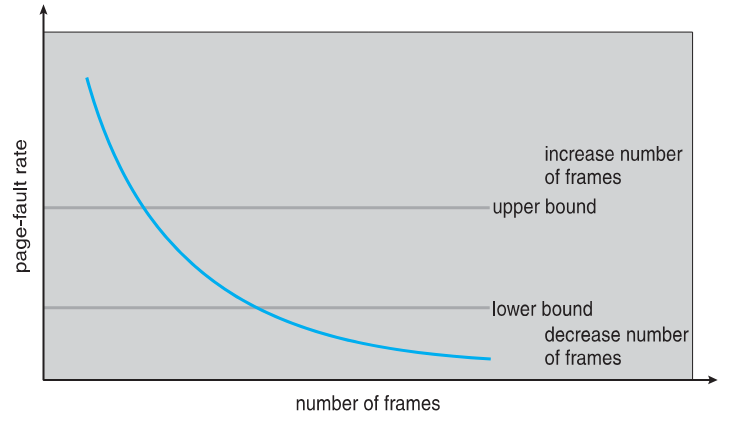
\includegraphics[width=1\linewidth]{content/OS_Internals/img/fmh.png}
    \captionof{figure}{PFF}
  \end{minipage}
\end{flushleft}


\section{Page Fault Frequency Algorithm}

Al differenza del Working Set, o Working Set Size, al posto di avere un timer
qui l'algoritmo si attiva soltanto quando ci sono page fault.
Dobbiamo ricordare quanto tempo intercorre tra due page fault. Frequenza bassa se
il tempo che intercorre è grande, e viceversa.

È attivato ad ogni evento di page fault, non al momento del riferimento alla pagina.

È basato sull'intervallo $\tau$, tempo che intercorre tra due page fault.


\begin{itemize}
  \item $\tau < C$ se il page fault è più grande di quella desiderata, aggiungi un frame al Resident Set del processo
  \item $\tau \geq C$ se la frequenza dei page fault è OK perché $\tau$ è grande, rimuovi un frame dal Resident Set del processo con bit a 0. Poi pulisci, setta a 0, il bit di riferimento di tutte le altre pagine nel Resident Set.
\end{itemize}



Supponimao che $\tau$ vada bene, ora abbiamo 2 modi per prendere decisioni: 2 azioni prendo quelli a zero e metto tutto a 1 il reference bit.

In rosso le vittime. In Verde la pagina referenziata con residence set a 1.


\begin{center}
  \begin{minipage}{0.45\linewidth}
    \centering
    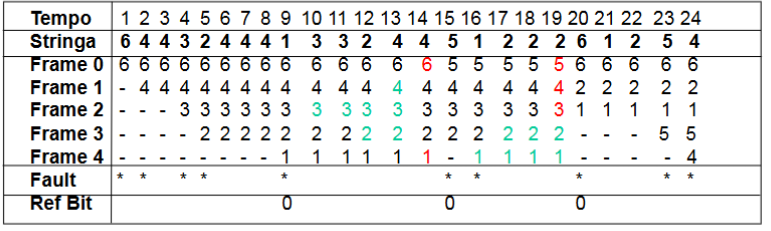
\includegraphics[width=\linewidth]{images/OS_internals/Main-memory/MM-esempio12.png}
    \captionof{figure}{Esempio di frequenza di page fault con C = 3}
  \end{minipage}%
  \hfill
  \begin{minipage}{0.45\linewidth}
    \centering
    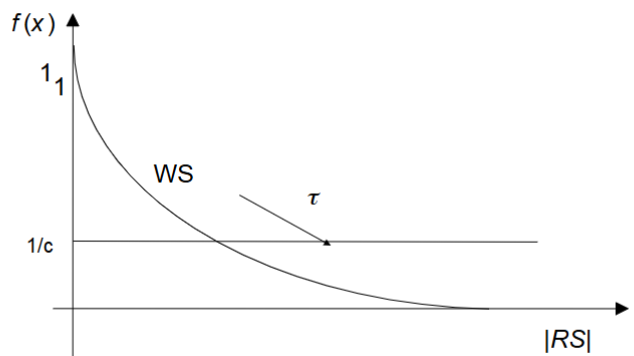
\includegraphics[width=\linewidth]{content/OS_Internals/images/2026-03-31-13-35-34.png}
  \end{minipage}
\end{center}

\paragraph{Spiegazione}
L'inizio di questo esempio è da considerarsi come un transitorio in questo esempio.


\begin{itemize}
  \item \textbf{Tempo 1-5} - si verificano page fault. Al tempo 4 faccio riferimento a 3, genero un page fault, e devo guardare quanto tempo è passato dall'ultimo page fault, ovvero 2 (tempo 4 - tempo 2) che è minore di C (3) quindi aggiungo una pagina al residence set.
  \item \textbf{Tempo 6-8} - non ci sono page fault essendo tutte le pagine referenziate in memoria.
  \item \textbf{Tempo 9} - si verifica un page fault, si attiva l'algoritmo nel caso che va bene, guardo quanto tempo è passato dall'ultimo page fault, ovvero 4 (tempo 9 - tempo 5) che è maggiore di C (3), non rimuovo nessuna pagina perché hanno tutti il refrence bit a 1 e a questo punto azzero tutti i reference bit. A questo punto però dobbiamo fare assunzioni se anche il valore appena aggiunto gli venga azzerato o meno il reference bit, in questo caso viene azzerato anche questo.
  \item \textbf{Tempo 10-13} - sono colorate in verde le pagine referenziate e il relativo reference bit è impostato ad 1.
  \item \textbf{Tempo 14} - a questo punto le pagine non referenziate se avviene page fault vengono eliminate
  \item \textbf{Tempo 15} - si fa riferimento a 5, non presente nel residence set, a questo punto avviene un page fault e si eliminano le pagine con residence bit a 0 e si aggiunge il 5 al residence set. A questo punto il residence set è diminuito (da 5 frame $\to$ 4 frame), e si azzerano tutti i reference bit, riportando la situazione all'inizio.
  \item \textbf{Tempo 16} - si fa riferimento nuovamente ad 1, si aggiunge al residence set e si setta a 1 il reference bit, azzerando gli altri
\end{itemize}

% Tempo 4, faccio riferiemnto a 3, page fault 2(tempo di ultimo page fault - tempo corrente)<3(C) aggiungo una pagina.

% tempo 9 si attiva l'algoritemo nel caso che va bene, non butto via nulla perchéhanno
% tutti refrence bit a 1, quindi aggiungo un freme ed azzero tutti i refrence bit. nel caso 9
% il refrence bit di \textit{1}, la pagina che ha creato page fault, è a zero o uno? si fanno delle assunzioni.

% nei tempi da 10-13 tempi sono messi a 1 i refrence bit per la pagine referenziate.
% In questo esempio abbiamo assunto che all'istante 9 viene messo anche 1 a zero e quindi a
% tempo 13 la sacrifico.

% all'istante 15 è diminuito il residence set, si è messo il 5 al posto di 6 per semplicità


\paragraph{}

\begin{itemize}
  \item \textbf{Working set}: pagine di un dato processo
  \item \textbf{WSS}: algoritmo per allocare dinamenicamnete il working set usando il tempo
  \item \textbf{Page Fault Frequency}: Usa la frequenza dei page fault per allocare dinamicamente il working set.
\end{itemize}



\subsubsection{Working Sets and Page Fault Rates}

\begin{center}
  \begin{minipage}{0.45\linewidth}
    Vi è una relazione diretta tra il working set di un processo e il suo tasso di page fault.
    Il working set cambia nel tempo.
  \end{minipage}%
  \hfill
  \begin{minipage}{0.45\linewidth}
    \centering
    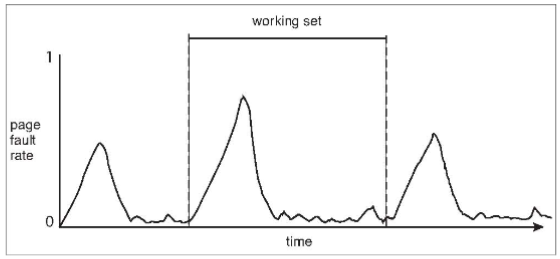
\includegraphics[width=\linewidth]{images/OS_internals/Main-memory/MM-esempio13.png}
  \end{minipage}
\end{center}


\section{Allocazione in memoria del kernel}

È trattata in maniera diversa rispetto alla memoria utente ed è spesso è allocata dal free-memory pool.

Il kernel richiede memoria per strutture di dimensioni variabili.
Parte della memoria del kernel deve essere contigua, vedi I/O device, dato che lavorano
con indirizzi fisici.

\section{Buddy System}

Alloca memoria da segmenti di dimensioni fisse costituiti da pagine fisicamente
contigue, solitamente allocate usando dimensioni di potenza di 2, si riduce il problema della
frammentazione esterna, ma quella interna rimane la quale sarà al massimo il 50\% (uso 65Kb al posto di 128Kb):

\begin{itemize}
  \item Soddisfa le richieste in unità di dimensioni potenza di 2
  \item La richiesta viene arrotondata alla potenza di 2 più vicina (10Kb $\to$ 16Kb)
  \item Quando è necessaria un'allocazione più piccola di quella disponibile,
        il chunk corrente viene diviso in due buddy della potenza di 2 successiva
        più bassa. Genero due parti eg. 128Kb $\to$ 2x64Kb $\to$ 4x32Kb $\to$ 8x16Kb
\end{itemize}

Questo precesso continua fino a quando una dimensione adatta è trovata.

\textbf{Vantaggio}: unisce rapidamente i chunk inutilizzati in chunk più grandi.\newline

\textbf{Svantaggio}: frammentazione esterna, ma effetto ridotto dato che si possono tentare di unire blocchi vicini, sono potenze di 2

\begin{center}
  \centering
  \begin{minipage}{1\linewidth}
    % Primo blocco: 50% dello spazio per il codice
    \begin{minipage}{0.65\linewidth}

      \paragraph{Esempio: } assumiamo che sia disponibile un chunk di 256KB, il kernel richiede 21KB.
      Viene diviso in $A_L$ e $A_R$ di 128KB ciascuno. Uno viene ulteriormente diviso in $B_L$ e $B_R$ di
      64KB. Uno viene ulteriormente diviso in $_CL$ e $C_R$ di 32KB ciascuno - uno viene usato per
      soddisfare la richiesta e 11KB di frammentazione interna.
    \end{minipage}% <-- IMPORTANTE: il simbolo % qui evita spazi bianchi extra
    \hfill
    \begin{minipage}{0.3\linewidth}
      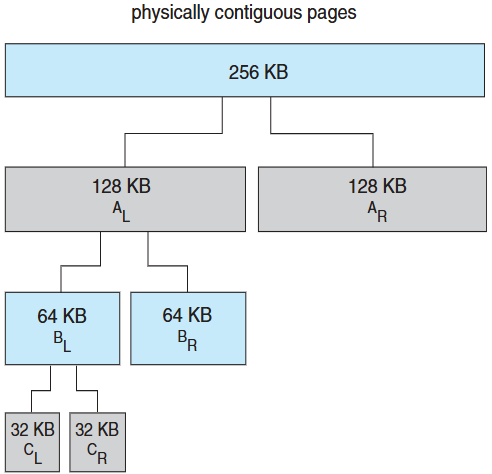
\includegraphics[width=1\linewidth]{images/OS_internals/Main-memory/MM-esempio14.png}

    \end{minipage}
  \end{minipage}
\end{center}


\section{Slab Allocator}

\begin{center}
  \centering
  \begin{minipage}{1\linewidth}
    % Primo blocco: 50% dello spazio per il codice
    \begin{minipage}{0.65\linewidth}
      Una strategia più flessibile utilizzata in ambiente linux in alternativa utilizza gli \textbf{slab} - composti da una o più pagine fisicamente contigue -
      e la \textbf{Cache} - costituita da uno o più slab.


      Una singola cache per ogni struttura dati univoca del kernel. Ogni cache è riempita
      con oggetti - istanziazioni della struttura dati.
      Quando la cache viene creata, viene riempita con oggetti marcati come \texttt{free}, altrimenti
      quando le strutture vengono memorizzate, gli oggetti sono marcati come \texttt{used}.

      Se uno slab è pieno di oggetti usati, il prossimo oggetto viene allocato da uno
      slab vuoto. Se non ci sono slab vuoti, viene allocato un nuovo slab.

      I vantaggi includono l'assenza di frammentazione e la soddisfazione rapida delle richieste di memoria

    \end{minipage}% <-- IMPORTANTE: il simbolo % qui evita spazi bianchi extra
    \hfill
    \begin{minipage}{0.3\linewidth}
      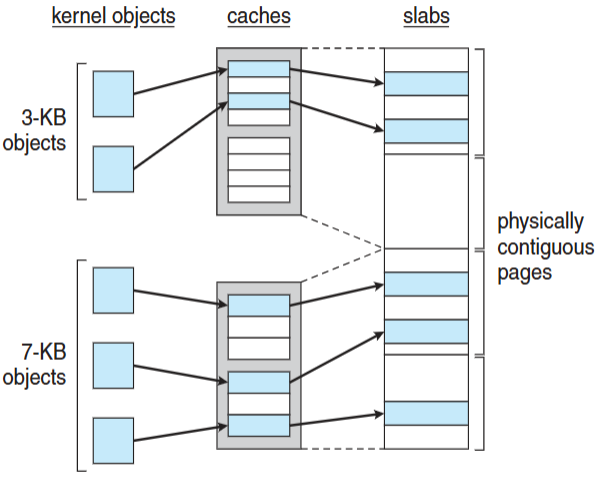
\includegraphics[width=1\linewidth]{images/OS_internals/Main-memory/MM-esempio15.png}

    \end{minipage}
  \end{minipage}
\end{center}

\paragraph{Esempio - Allocatore Slab in Linux}

Per esempio, il descrittore di processo è di tipo \verb|struct task_struct| con
approssimativamente 1.7KB di memoria.

Nuovo task $\to$ alloca una nuova struttura dalla cache. Utilizzerà una
\verb|struct task_struct| libera esistente.

Lo slab può essere in tre possibili stati:

\begin{enumerate}
  \item Full - tutto usato
  \item Empty - tutto libero
  \item Partial - alcuni liberi, alcuni usati
\end{enumerate}

Su richiesta, l'allocatore slab

\begin{enumerate}
  \item Usa uno struct libero in uno slab parziale
  \item Se nessuno, ne prende uno da uno slab vuoto
  \item Se non c'è uno slab vuoto, ne crea uno nuovo vuoto
\end{enumerate}

Lo slab è nato in Solaris, ora è diffuso sia per il kernel mode che per la memoria utente in
vari SO. Linux 2.2 aveva SLAB, ora ha sia gli allocatori SLOB che SLUB


\section{Prepaging}

Per caricare un processo, si deve leggere l'eseguibile. Siamo passati da caricarlo tutto
fino al caricarlo durante i page fault (pure/partial demangin page).
% In ogni caso le prime pagine avranno page fault, in questo caso prepaginare si intende
% caricare la pagina prima che capita il page fault. Page fault 1? carico anche la 2 e 3
% sperando che mi servano riducendo i futuri page fault.


Per ridurre il grande numero di page fault che si verificano all'avvio del processo,
il \textbf{prepaging} può essere utilizzato per caricare più della semplice pagina richiesta.
Si precaricano tutte o alcune delle pagine che un processo necessiterà, prima che vengano referenziate,
ma se le pagine precaricate non vengono utilizzate, l'I/O e la memoria sono stati sprecati.

\paragraph{Esempio: } Assumiamo che \textit{s} pagine sono precaricate e $\alpha$ delle pagine viene
utilizzato

\begin{itemize}
  \item \textit{s} costo di $s \cdot \alpha$ risparmia page fault > o < del costo del prepaging. $s \cdot (1 - \alpha)$ pagine non necessarie?
  \item $\alpha$ vicino a zero $\to$ il prepaging perde
\end{itemize}

\section{Dimensione della Pagina}

Talvolta i progettisti di SO hanno una scelta, specialmente se operano su CPU custom-built.
Per dimensionare correttamente le pagine dobbimao tenere conto di diversi fattori, tra cui:

% La selezione della dimensione della pagina deve prendere in considerazione:

\begin{itemize}
  \item Frammentazione interna $\to$ più grande è la pagina e più frammentazione interna avremo. Meglio piccole.
  \item Dimensione della tabella delle pagine $\to$ più grande è la pagina e meno righe nella page table, quindi meno memoria per la page table. Meglio grandi.
  \item Risoluzione
  \item Overhead dell'I/O $\to$ più grande è la pagina e più ammortizzo il costo di I/O. Meglio grandi.
  \item Numero di page fault $\to$ più grande è la pagina e meno page fault
  \item Località $\to$ più grande è la pagina e più probabilmente avrò località, ma se è troppo grande rischio di avere un tasso di page fault più alto dato che una data funzione è presente in una pagina non caricata.
  \item Dimensione ed efficacia del TLB -> meglio pagine più grandi così con lo stesso hw "vede" più memoria (TLB reach)
\end{itemize}

Dire che aumentare la dimensione della pagina riduce il numero di page fault non è sempre vero,
dato che il page fault è decisa da:

\begin{gather*}
  \text{Page Fault} = f(m, A, w) \\
  \text{Dove: } \textit{m} \text{ è il numero di frame, } \textit{A} \text{ è l'algoritmo di sostituzione e } \textit{w} \text{ è la stringa di riferimento}
\end{gather*}

\paragraph{}


Sempre potenze di 2, solitamente nell'intervallo $2^{12}\,(4096 \text{byte})$ a $2^{22}\,(4194304 \text{byte})$.
In media, crescente nel tempo.

\section{TLB Reach}
\textbf{TLB Reach} - La quantità di memoria accessibile dal TLB.

\begin{equation*}
  \text{TLB Reach} = \text{TLB Size} \times \text{Page Size}
\end{equation*}
\paragraph{}

Idealmente, il working set di ogni processo dovrebbe essere memorizzato nel TLB, altrimenti c'è
un alto grado di page fault.


\begin{itemize}
  \item \textbf{Aumentare la Dimensione della Pagina: } Questo può portare a un aumento della frammentazione interna poiché non tutte
        le applicazioni richiedono una grande dimensione di pagina
  \item \textbf{Fornire Dimensioni di Pagina Multiple: } Questo consente alle applicazioni che
        richiedono dimensioni di pagina più grandi l'opportunità di utilizzarle senza un aumento della
        frammentazione
\end{itemize}

\paragraph{Esempio: Struttura del programma}

\texttt{int[128,128] data;} - ogni riga è memorizzata in una pagina (512 byte).


\begin{center}
  \centering
  \begin{minipage}{0.85\linewidth}
    % Primo blocco: 50% dello spazio per il codice
    \begin{minipage}{0.45\linewidth}
      \begin{minted}[breaklines]{c}
// Program 1
  for (j = 0; j <128; j++) 
    for (i = 0; i < 128; i++) 
      data[i,j] = 0;
\end{minted}
      $128 \times 128$ page faults. Ogni accesso ha fatto accesso ad una pagina diversa. Qualsiasi sia il working set avrà sempre page fault.
    \end{minipage}% <-- IMPORTANTE: il simbolo % qui evita spazi bianchi extra
    \hfill
    \begin{minipage}{0.45\linewidth}
      \begin{minted}[breaklines]{c}
// Program 2
  for (i = 0; i <128; i++) 
    for (j = 0; j < 128; j++) 
      data[i,j] = 0;
\end{minted}
      $128 \times 128$ page faults. 1 page fault per ogni pagina.
    \end{minipage}
  \end{minipage}
\end{center}

\section{I/O interlock}

\begin{center}
  \centering
  \begin{minipage}{1\linewidth}
    % Primo blocco: 50% dello spazio per il codice
    \begin{minipage}{0.65\linewidth}
      \textbf{I/O Interlock} - Le pagine devono talvolta essere bloccate in memoria.
      Consideriamo l'I/O - Le pagine che vengono utilizzate per copiare
      un file da un dispositivo devono essere bloccate ed evitare di essere selezionate per l'espulsione da un algoritmo
      di sostituzione delle pagine

      \textbf{Pinning} delle pagine per bloccarle in memoria.

    \end{minipage}% <-- IMPORTANTE: il simbolo % qui evita spazi bianchi extra
    \hfill
    \begin{minipage}{0.3\linewidth}
      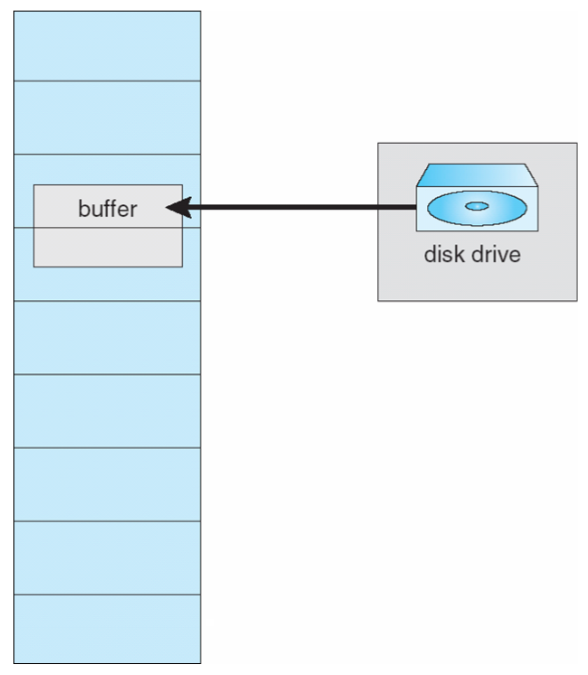
\includegraphics[width=\textwidth]{images/OS_internals/Main-memory/MM-esempio16.png}
    \end{minipage}
  \end{minipage}
\end{center}

\subsection{Esempio Windows}

Utilizza paginazione su richiesta con clustering. Il clustering carica le pagine
circostanti alla pagina che genera il fault. Ai processi vengono assegnati un working set minimo e un working set
massimo. Il working set minimo è il numero minimo di pagine che
il processo è garantito di avere in memoria. Un processo può essere assegnato fino a un numero di pagine pari al suo working set
massimo. Quando la quantità di memoria libera nel sistema scende sotto una
soglia, viene eseguita automaticamente la riduzione del working set
per ripristinare la quantità di memoria libera. La riduzione del working set rimuove pagine dai processi che hanno
pagine in eccesso rispetto al loro working set minimo


\subsection{Esempio Solaris}


\begin{center}
  \centering
  \begin{minipage}{1\linewidth}
    % Primo blocco: 50% dello spazio per il codice
    \begin{minipage}{0.65\linewidth}
      Mantiene una lista di pagine libere da assegnare ai processi che generano fault.
      Lotsfree - parametro di soglia (quantità di memoria libera) per iniziare il paging.
      Desfree - parametro di soglia per aumentare il paging. Minfree - parametro di
      soglia per iniziare lo swapping. Il paging viene eseguito dal processo pageout.
      Pageout scansiona le pagine usando un algoritmo clock modificato. Scanrate è la velocità con
      cui le pagine vengono scansionate. Questo varia da slowscan a fastscan. Pageout viene
      chiamato più frequentemente a seconda della quantità di memoria libera disponibile.
      Il paging con priorità dà priorità alle pagine di codice del processo

    \end{minipage}% <-- IMPORTANTE: il simbolo % qui evita spazi bianchi extra
    \hfill
    \begin{minipage}{0.3\linewidth}
      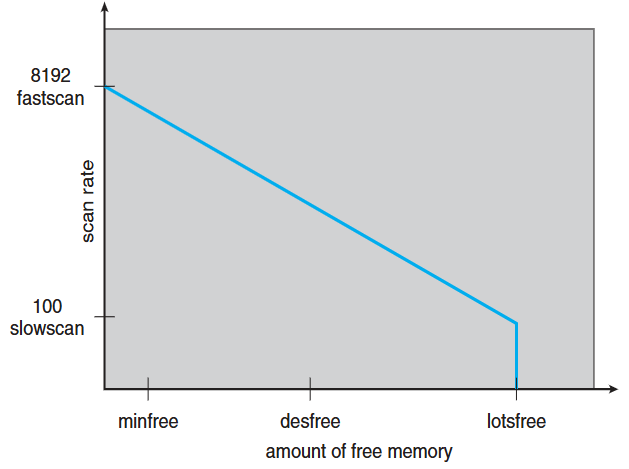
\includegraphics[width=\textwidth]{images/OS_internals/Main-memory/MM-esempio17.png}
    \end{minipage}
  \end{minipage}
\end{center}


\section{Performance del Demand Paging}

Fasi della Paginazione su Richiesta (caso peggiore)

\begin{enumerate}
  \setlength{\itemsep}{0pt}
  \item Trap al sistema operativo
  \item Salva i registri utente e lo stato del processo
  \item Determina che l'interruzione è stata causata da un page fault
  \item Verifica che il riferimento alla pagina sia legale e determina la posizione della pagina sul disco
  \item Emetti una lettura dal disco a un frame libero:
        \begin{itemize}
          \setlength{\itemsep}{0pt}
          \item Attendi in una coda per questo dispositivo fino a quando la richiesta di lettura non viene soddisfatta
          \item Attendi il tempo di seek e/o latenza del dispositivo
          \item Inizia il trasferimento della pagina a un frame libero
        \end{itemize}
  \item Mentre aspetti, assegna la CPU a qualche altro utente
  \item Ricevi un'interruzione dal sottosistema I/O del disco (I/O completato)
  \item Salva i registri e lo stato del processo per l'altro utente
  \item Determina che l'interruzione è stata causata dal disco
  \item Correggi la tabella delle pagine e altre tabelle per mostrare che la pagina è ora in memoria
  \item Attendi che la CPU venga assegnata di nuovo a questo processo
  \item Ripristina i registri utente, lo stato del processo e la nuova tabella delle pagine, quindi riprendi l'istruzione interrotta
\end{enumerate}





% \begin{center}
%   \centering
%   \begin{minipage}{1\linewidth}
%     % Primo blocco: 50% dello spazio per il codice
%     \begin{minipage}{0.65\linewidth}
%       \begin{enumerate}
%         \item Trap to the operating system
%         \item Save the user registers and process state
%         \item Determine that the interrupt was a page fault
%         \item Check that the page reference was legal and determine the location of the page on the disk
%         \item Issue a read from the disk to a free frame:
%               \begin{itemize}
%                 \item Wait in a queue for this device until the read request is serviced
%                 \item Wait for the device seek and/or latency time
%                 \item Begin the transfer of the page to a free frame
%               \end{itemize}
%         \item While waiting, allocate the CPU to some other user
%         \item Receive an interrupt from the disk I/O subsystem (I/O completed)
%         \item Save the registers and process state for the other user
%         \item Determine that the interrupt was from the disk
%         \item Correct the page table and other tables to show page is now in memory
%         \item Wait for the CPU to be allocated to this process again
%         \item Restore the user registers, process state, and new page table, and then resume the interrupted instruction
%       \end{enumerate}

%     \end{minipage}% <-- IMPORTANTE: il simbolo % qui evita spazi bianchi extra
%     \hfill
%     \begin{minipage}{0.3\linewidth}
%       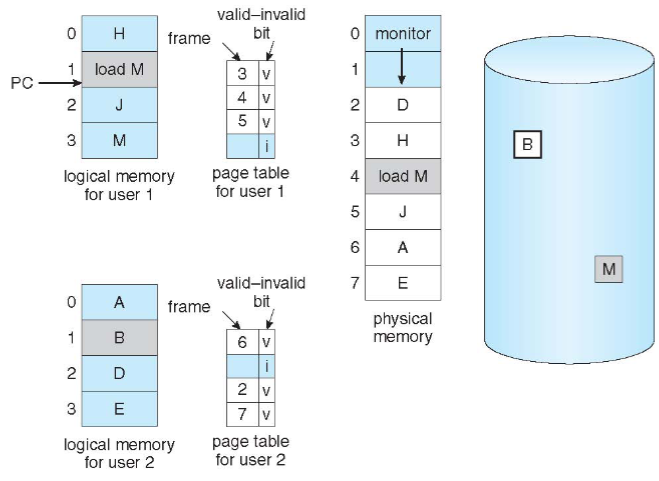
\includegraphics[width=\textwidth]{images/OS_internals/Main-memory/MM-esempio18.png}
%       \captionof{figure}{Need for page replacement}
%     \end{minipage}
%   \end{minipage}
% \end{center}


% VERSIONE GEMINI

\begin{flushleft} % Sostituisce center per allineare l'intero blocco a sinistra
  \begin{minipage}{1\linewidth}
    % Primo blocco: 65% dello spazio per il codice
    \begin{minipage}{0.65\linewidth}
      \raggedright % <-- Questo comando forza il testo ad allinearsi a sinistra
      \begin{enumerate}
        \item Trap al sistema operativo
        \item Salva i registri utente e lo stato del processo
        \item Determina che l'interruzione è stata causata da un page fault
        \item Verifica che il riferimento alla pagina sia legale e determina la posizione della pagina sul disco
        \item Emetti una lettura dal disco a un frame libero:
              \begin{itemize}
                \item Attendi in una coda per questo dispositivo fino a quando la richiesta di lettura non viene soddisfatta
                \item Attendi il tempo di seek e/o latenza del dispositivo
                \item Inizia il trasferimento della pagina a un frame libero
              \end{itemize}
        \item Mentre aspetti, assegna la CPU a qualche altro utente
        \item Ricevi un'interruzione dal sottosistema I/O del disco (I/O completato)
        \item Salva i registri e lo stato del processo per l'altro utente
        \item Determina che l'interruzione è stata causata dal disco
        \item Correggi la tabella delle pagine e altre tabelle per mostrare che la pagina è ora in memoria
        \item Attendi che la CPU venga assegnata di nuovo a questo processo
        \item Ripristina i registri utente, lo stato del processo e la nuova tabella delle pagine, quindi riprendi l'istruzione interrotta
      \end{enumerate}
    \end{minipage}% <-- IMPORTANTE: il simbolo % qui evita spazi bianchi extra
    \hfill
    \begin{minipage}{0.3\linewidth}
      \centering % Centra l'immagine all'interno della sua colonna (opzionale)
      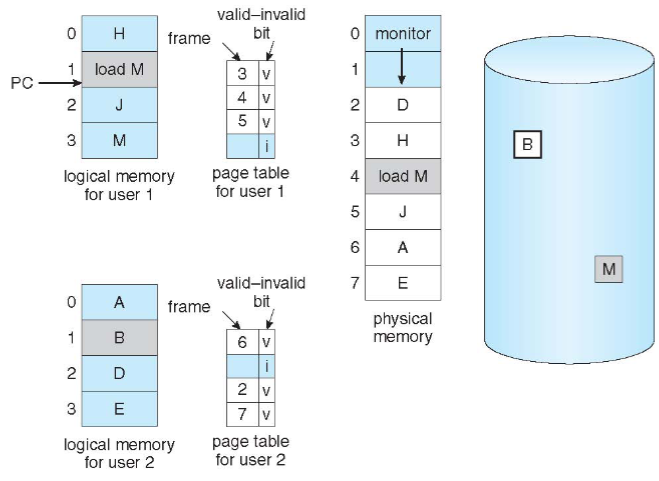
\includegraphics[width=\textwidth]{images/OS_internals/Main-memory/MM-esempio18.png}
    \end{minipage}
  \end{minipage}
\end{flushleft}

Cosa è cambiato esattamente: Sostituito \\begin{center} con \\begin{flushleft}:
Questo sposta l'intero blocco principale (quello largo 1\\linewidth) verso il
margine sinistro della pagina, invece di tenerlo in mezzo.

Rimosso il comando \\centering globale: Era ridondante e causava l'allineamento
centrale non desiderato del testo.

Aggiunto \\raggedright: Inserito subito dopo l'apertura della prima minipage,
dice a LaTeX di allineare tutto il contenuto di quella colonna a sinistra,
disabilitando la giustificazione automatica che a volte crea spazi vuoti
antiestetici nelle colonne strette.


\subsection{Priority Allocation}

Utilizza uno schema di allocazione proporzionale usando le priorità piuttosto
che la dimensione.
Se il processo $P_i$ genera un page fault:
\begin{itemize}
  \item seleziona per la sostituzione uno dei suoi frame
  \item seleziona per la sostituzione un frame da un processo con
        numero di priorità inferiore
\end{itemize}

\subsection{Compressione della Memoria}

Un'alternativa alla paginazione è la \textbf{compressione della memoria}.


\textbf{Compressione della memoria} - invece di effettuare il paging out dei frame modificati nello spazio di swap,
comprimi diversi frame in un singolo frame, consentendo al sistema di ridurre
l'utilizzo della memoria senza ricorrere allo swapping delle pagine.

Considera la seguente free-frame-list costituita da 6 frame




\begin{center}
  \centering
  \begin{minipage}{0.75\linewidth}

    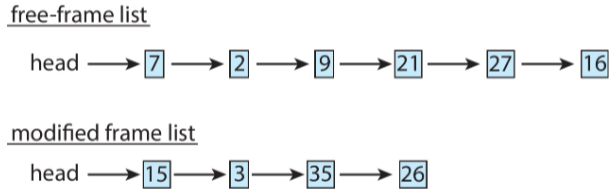
\includegraphics[width=0.47\textwidth]{images/OS_internals/Main-memory/MM-esempio19.png}
    \hfill
    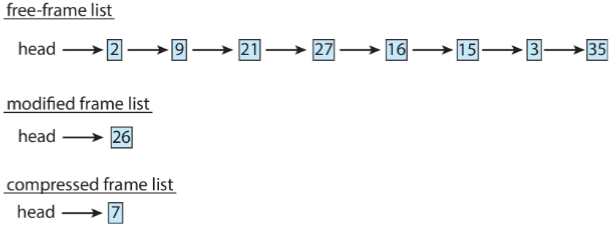
\includegraphics[width=0.47\textwidth]{images/OS_internals/Main-memory/MM-esempio20.png}

  \end{minipage}
\end{center}

Supponiamo che questo numero di frame liberi scenda sotto una certa soglia che
attiva la sostituzione delle pagine. L'algoritmo di sostituzione (ad esempio, un algoritmo di approssimazione
LRU) seleziona quattro frame -- 15, 3, 35 e 26 da inserire nella free-frame
list. Prima posiziona questi frame in una modified-frame list. Tipicamente, la
modified-frame list verrebbe poi scritta nello spazio di swap, rendendo i frame
disponibili alla free-frame list. Una strategia alternativa è comprimere un
certo numero di frame{\\mdash}diciamo, tre{\\mdash}e memorizzare le loro versioni compresse in
un singolo frame di pagina.



\chapter{Approfondimento sulla Memoria Virtuale}

\section{Swapping delle Pagine}


% Cosa si intende con swapping? gioco che coinvolge Ram e disco, fino ad ora abbiamo
% parato di memoria primaria.
% Scambio di contenuto tra backing store una pare del disco che non serve ad
% ospitare il file syetma ma che serve a fare da memoria aggiuntiva
% per aiutare la ram.

% Un processo può essere fermo per qualche cosa, occupa memoria in ram,
% Toglilo dalla memoria swap out o roll out e salviamolo sul backing store
% e in questo meodo la ram viene liberata. Usato da altri processi per
% esparndersi o altri programmi di venir eseguito.

Fino ad ora abbiamo parlato di memoria primaria. Ora introduciamo anche la
memoria secondaria, un disco veloce, chiamato \textbf{backing store} utilizzato
come memoria aggiuntiva.


Un processo, se è fermo per I/O o altro, può essere
temporaneamente spostato dalla memoria all'HD e poi riportato in memoria per
continuare l'esecuzione. Lo spazio di memoria logico totale dei processi può
superare la memoria fisica. In questo modo viene liberato spazio in RAM per
eseguire altri processi o per far espandere processi già esistenti.

\paragraph{HD - Backing store} - disco veloce abbastanza grande da contenere copie di tutte
le immagini di memoria di tutti gli utenti; deve fornire accesso diretto a queste
immagini di memoria.


\paragraph{Roll out, roll in} - variante dello swapping usata negli algoritmi di
scheduling basati sulla priorità; il processo a bassa priorità viene rimosso dalla
memoria (swap out) in modo che il processo a priorità più alta possa essere caricato ed eseguito.

\paragraph{}

La parte principale del tempo di swap è il tempo di trasferimento; il tempo totale di trasferimento è direttamente
proporzionale alla quantità di memoria trasferita. Il sistema mantiene una \textbf{ready queue} di processi pronti all'esecuzione che
possiedono immagini di memoria su disco.

\begin{center}
  \centering
  \begin{minipage}{1\linewidth}
    % Primo blocco: 50% dello spazio per il codice
    \begin{minipage}{0.65\linewidth}
      Il processo che è stato rimosso (swap out) deve tornare agli stessi indirizzi fisici?

      Di solito no, ma dipende dal metodo di binding degli indirizzi; occorre anche considerare l'I/O in attesa verso/dalla memoria del processo.
      Ogni OS può decidere come gestire il metodo di swap:

      \begin{itemize}
        \item Swapping normalmente disabilitato
        \item Avviato se la quantità di memoria allocata supera una soglia
        \item Disabilitato nuovamente quando la domanda di memoria scende sotto la soglia
      \end{itemize}
    \end{minipage}% <-- IMPORTANTE: il simbolo % qui evita spazi bianchi extra
    \hfill
    \begin{minipage}{0.3\linewidth}
      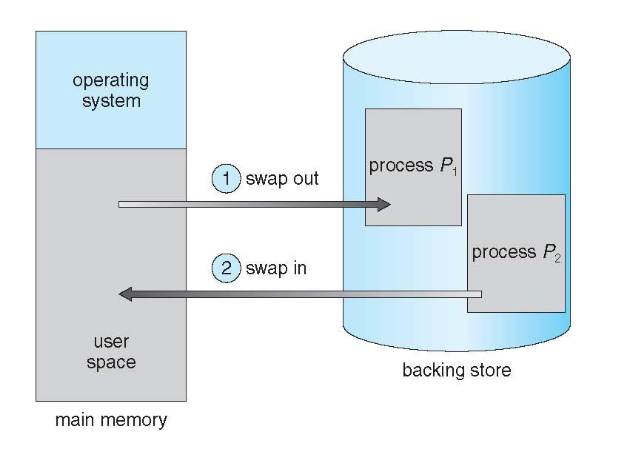
\includegraphics[width=1\linewidth]{content/OS_Internals/img/dfbngt.png}
      \captionof{figure}{Processo di swapping}
    \end{minipage}
  \end{minipage}
\end{center}

QUando lo riporto dentro posso portarlo in un posti diverso, è meno vincolato mettendolo in
un'altra partizione solo se gli indirizzi sono rilocabili e dipende da come hai fatto binding
degli indirizzi.


\newpage
\subsection{Tempo di Context Switch con lo Swapping}



Se il prossimo processo da eseguire sulla CPU non è in memoria e la RAM è piena,
occorre effettuare lo swap out di un processo e lo swap in del processo target.
Il tempo di context switch può quindi essere molto elevato, ovvero la latenza
per il trasferimento dati verso l'HD.

\paragraph{Esempio: } processo da 100MB in swap verso l'hard disk con velocità di
trasferimento di 50MB/sec:

\begin{itemize}
  \item[] Tempo di swap out di 2 secondi
  \item[] Più swap in di un processo delle stesse dimensioni
  \item[] Tempo totale del componente di swapping nel context switch: 4 s
\end{itemize}

È possibile ridurre il tempo sapendo quanta memoria viene effettivamente usata. Chiamate di sistema per informare l'OS sull'uso della memoria tramite
\verb|request_memory()| e \verb|release_memory()|.

\begin{center}
  \centering
  \begin{minipage}{1\linewidth}
    % Primo blocco: 50% dello spazio per il codice
    \begin{minipage}{0.65\linewidth}

      \paragraph{Altri vincoli: } se un task ha I/O in attesa non può essere rimosso (swap out), poiché l'I/O avverrebbe sul processo sbagliato; oppure si trasferisce sempre l'I/O nello spazio kernel e poi al dispositivo I/O, ma questo causa il cosiddetto double buffering, aggiungendo overhead.


      Allora come funziona nei \textbf{sistemi operativi moderni}?

      \begin{itemize}
        \item[] Lo swap viene attivato solo quando la memoria libera è quasi esaurita
        \item[] Con la memoria a pagine si scambiano intere pagine dentro e fuori dalla RAM
        \item[] Le pagine spostate su disco vengono in genere salvate in un “file di paging”
      \end{itemize}
    \end{minipage}% <-- IMPORTANTE: il simbolo % qui evita spazi bianchi extra
    \hfill
    \begin{minipage}{0.3\linewidth}
      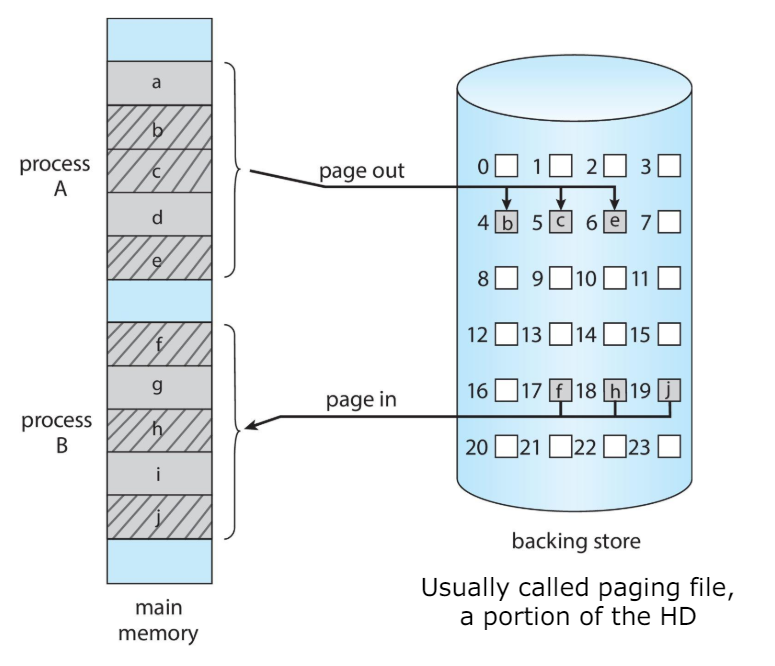
\includegraphics[width=1\linewidth]{content/OS_Internals/img/ndgf.png}
      \captionof{figure}{Swapping con paginazione}
    \end{minipage}
  \end{minipage}
\end{center}

Oltre che per i singoli processi, la tecnica dello swapping è implementata anche a livello di
pagine. Non tutte le pagine di un processo devono stare in memoria.


\subsection{Swapping sui Sistemi Mobili}

% Non si fa, si fa una cosa più semplice: chiedere all'applicazione di salvarsi i dati
% altrimenti il kernel la termina.

Lo swapping non viene tipicamente usato perché lo storage è piccolo, il flash drive ha un numero limitato di cicli di scrittura e il bus tra la memoria flash e la CPU è limitato.

Quindi, invece di usare lo swapping quando la memoria libera è bassa:

\begin{itemize}
  \item \textbf{iOS} chiede alle app di cedere volontariamente la memoria allocata; i dati in sola lettura vengono eliminati e ricaricati dal flash se necessario. Il mancato rilascio può portare alla terminazione.
  \item \textbf{Android} termina le app in caso di memoria libera insufficiente, ma prima salva lo stato dell'applicazione nel flash per un riavvio rapido.
\end{itemize}


Entrambi i sistemi operativi supportano la paginazione come discusso di seguito.



\section{Struttura della Tabella delle Pagine}

Le strutture di memoria per la paginazione possono diventare enormi con metodi diretti. Si consideri uno spazio di indirizzamento logico a 32 bit, con pagine da 4KB: la tabella avrebbe 1 milione di voci e lo spazio totale per OGNI processo è di 4MB solo per ottenere lo spazio di indirizzamento fisico, i quali devono essere contigui.

Una soluzione semplice è dividere la tabella delle pagine in unità più piccole e caricarla solo parzialmente:

\begin{enumerate}
  \item Shared Pages
  \item Paginazione Gerarchica
  \item Tabelle delle Pagine con Hashing
  \item Tabelle delle Pagine Invertite
\end{enumerate}

\subsection{Shared Pages}

\begin{center}
  \centering
  \begin{minipage}{1\linewidth}
    % Primo blocco: 50% dello spazio per il codice
    \begin{minipage}{0.65\linewidth}

      \subsubsection{Shared code}
      Una sola copia in modalità read-only (reentrant), è condivisa tra i processi (eg. text editors, compilers, windows systems).
      Il concetto è simile a thread multipli che condividono lo stesso process space.

      Inoltre è anche molto utile per le comunicazioni interprocesso (IPC), se la condivisione di pagine read-write è consentita.

      \subsubsection{Codice privato e dati}

      Ogni processo tiene una copia privata del codice e dei dati.
      Le pagine di codice e dati privati possono apparire ovunque nella logical address space.

    \end{minipage}% <-- IMPORTANTE: il simbolo % qui evita spazi bianchi extra
    \hfill
    \begin{minipage}{0.3\linewidth}
      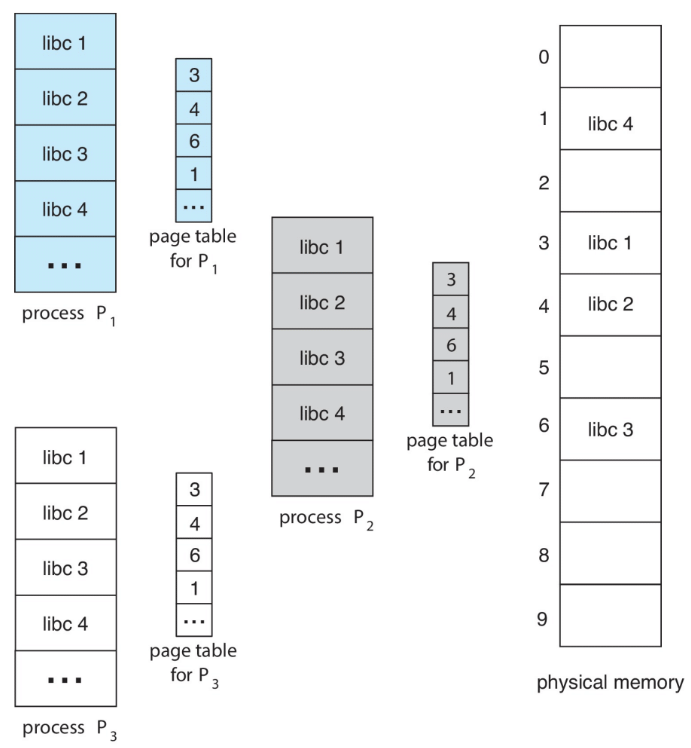
\includegraphics[width=1\linewidth]{images/OS_internals/Main-memory/MM-esempio1.png}

    \end{minipage}
  \end{minipage}
\end{center}


\subsection{Paginazione gerarchica}


\begin{center}
  \centering
  \begin{minipage}{1\linewidth}
    % Primo blocco: 50% dello spazio per il codice
    \begin{minipage}{0.75\linewidth}

      Con questo metodo si suddivide lo spazio di indirizzamento logico in più tabelle delle pagine. Una tecnica semplice è la tabella delle pagine a due livelli: in questo modo si carica solo la sezione di interesse.


      Con indirizzi a 32 bit e pagine da 4 KB, l'indirizzo logico si divide in:

    \end{minipage}% <-- IMPORTANTE: il simbolo % qui evita spazi bianchi extra
    \hfill
    \begin{minipage}{0.25\linewidth}
      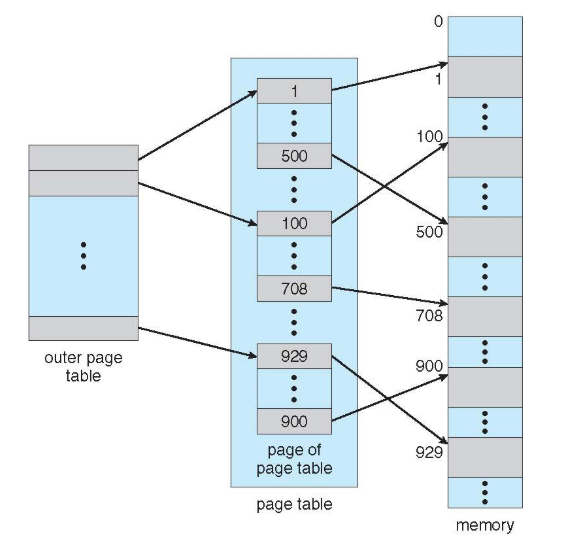
\includegraphics[width=1\linewidth]{content/OS_Internals/img/sbdf.png}

    \end{minipage}
  \end{minipage}
\end{center}



\begin{itemize}
  \item un numero di pagina di 20 bit, suddiviso in due parti da 10 bit ciascuna:
        \begin{itemize}
          \item[] p1 per selezionare la pagina delle page table, cioè la \textbf{pagina esterna}
          \item[] p2 per selezionare la riga specifica del “blocco” di page table, la \textbf{pagina interna}
        \end{itemize}
  \item un offset di pagina di 12 bit
\end{itemize}

\begin{figure}[htbp]
  \centering
  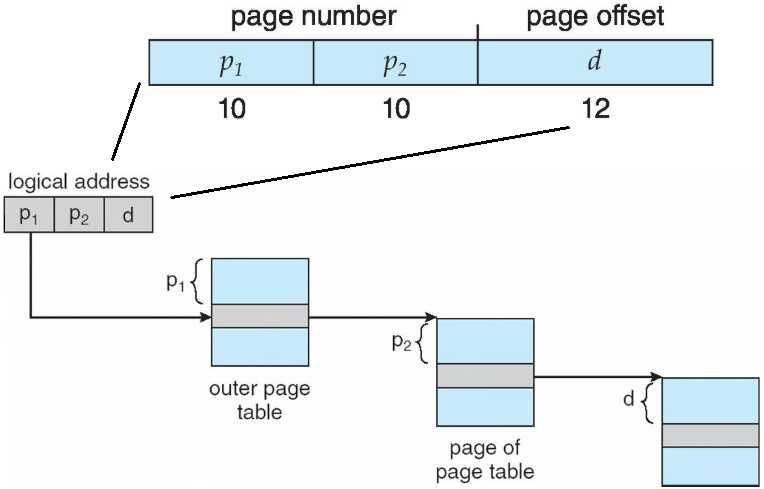
\includegraphics[width=0.3\linewidth]{content/OS_Internals/img/mu.png}
\end{figure}

\textbf{ATTENZIONE ERRORE: non è 10 10 12 bensì 10 12 10
  ETA da cambiare perché è su 3 livelli e non 2}


\subsubsection{Spazio di Indirizzamento Logico a 64 bit}


\begin{center}
  \centering
  \begin{minipage}{1\linewidth}
    % Primo blocco: 50% dello spazio per il codice
    \begin{minipage}{0.65\linewidth}

      Anche uno schema di paginazione a due livelli potrebbe non essere sufficiente; se la dimensione della pagina è ancora 4 KB, la tabella delle pagine ha $2^{52}$ voci e le tabelle delle pagine interne potrebbero essere $2^{10}$, vedi figura affianco.

    \end{minipage}% <-- IMPORTANTE: il simbolo % qui evita spazi bianchi extra
    \hfill
    \begin{minipage}{0.3\linewidth}
      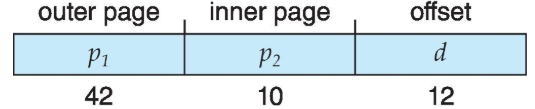
\includegraphics[width=1\linewidth]{content/OS_Internals/img/ndg.png}


    \end{minipage}
  \end{minipage}
\end{center}


\begin{center}
  \centering
  \begin{minipage}{1\linewidth}
    % Primo blocco: 50% dello spazio per il codice
    \begin{minipage}{0.65\linewidth}

      La tabella delle pagine esterna ha $2^{42}$ voci, ovvero 4 terabyte per processo! Una soluzione potrebbe essere aggiungere un ulteriore livello di tabella delle pagine esterna, vedi figura affianco.\newline
      Il problema qui è che sono necessari 4 accessi in memoria per ottenere una singola posizione di memoria fisica, il che non è una soluzione brillante.

    \end{minipage}% <-- IMPORTANTE: il simbolo % qui evita spazi bianchi extra
    \hfill
    \begin{minipage}{0.3\linewidth}
      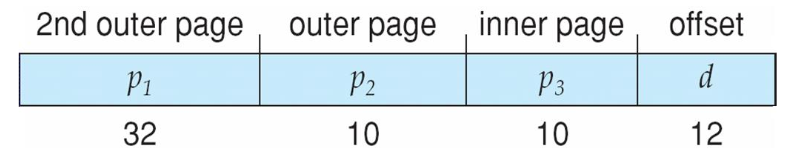
\includegraphics[width=1\linewidth]{content/OS_Internals/img/db.png}


    \end{minipage}
  \end{minipage}
\end{center}




\subsection{Tabelle delle Pagine con Hashing}
Gli spazi di indirizzamento comuni sono $> 32$ bit. Il numero di pagina virtuale viene sottoposto a hashing in una tabella delle pagine; questa tabella contiene un elenco di elementi a cui è stato applicato lo stesso hash.

\begin{minipage}{0.9\linewidth}
  % Primo blocco: 50% dello spazio per il codice
  \begin{minipage}{0.65\linewidth}

    Ogni elemento contiene:

    \begin{itemize}
      \item il numero di pagina virtuale
      \item il valore del frame di pagina mappato
      \item un puntatore all'elemento successivo
    \end{itemize}
  \end{minipage}% <-- IMPORTANTE: il simbolo % qui evita spazi bianchi extra
  \hfill
  \begin{minipage}{0.3\linewidth}
    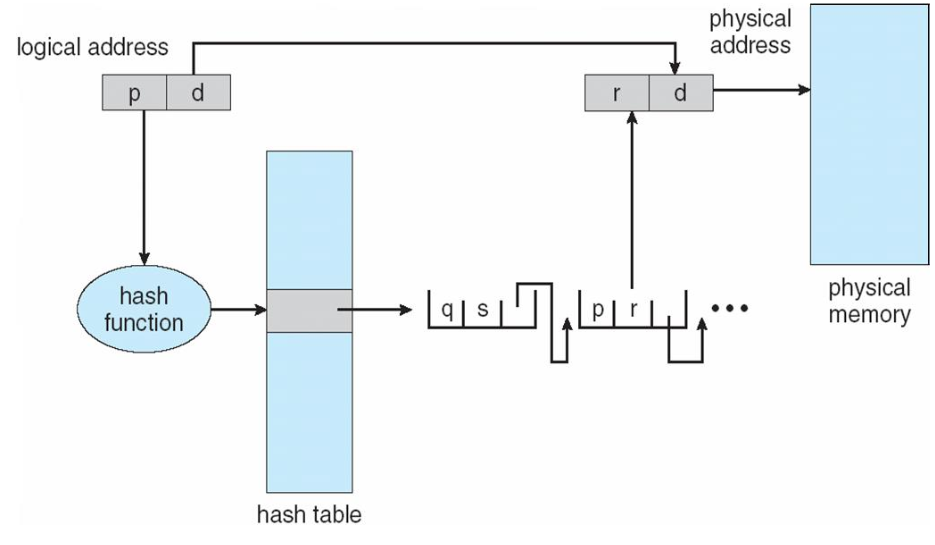
\includegraphics[width=1\linewidth]{content/OS_Internals/img/ngf.png}
    \captionof{figure}{Tabella delle pagine con hashing}

  \end{minipage}
\end{minipage}


Se si dispone di uno spazio di indirizzamento a 64 bit, 12 bit sono per l'offset, quindi 52 per l'indirizzo di pagina. Si può usare una tabella hash da 4KB ($2^{12}$), che tipicamente si adatta a una singola pagina e rimane sempre in memoria per ciascun processo.

Si accede alla pagina specifica tramite essa. Se tutta la memoria viene usata dal processo, questo non è efficiente. Tuttavia, nella stragrande maggioranza dei casi nessun processo utilizzerà tutti i $2^{52}$ pagine.


Ovviamente di possono avere collisioni, ma non è un grosso problema se la tabella hash è abbastanza grande.
Altrimenti, possono utilizzare \textbf{open addressing} (cerca un altro posto) o \textbf{linear chaining} (una lista).

\subsection{Tabella delle Pagine Invertita}

% \textbf{Bravissima da l'indice è il frame e il contenuto il n di pagina
% Perché? gli spazzi di indirizzamenteo sono >> della RAM, supponiamo di avere 4 processi 
% da 4GB ogniuno 40GB e tante tabelle delle pagine e se ho solo 4GB di ram, non 
% ci stanno tutti.
% Facciamo un vettore parallelo alla ram, il vettor e ha una riga per ogni riga di ram 
% occupata!  e non sui 64bit
% La tabella delle pagine è una singola per tutte, risparmi anceh su questo.
% Va meglio in termini di memoria ma fa peggio di tempo, ricerca linear!
% Mettiamoci una hash table davanti. inverted page table fa una hash table più furba senza le liste linkate
% }

\begin{center}
  \centering
  \begin{minipage}{1\linewidth}
    % Primo blocco: 50% dello spazio per il codice
    \begin{minipage}{0.65\linewidth}


      Invece di avere una tabella delle pagine per ogni processo che tiene traccia di tutte le pagine logiche possibili, si ha un'unica voce per ogni pagina reale della memoria!

      Ogni voce consiste nell'indirizzo virtuale della pagina memorizzata in quella locazione di memoria reale, con informazioni sul processo che possiede quella pagina.

    \end{minipage}% <-- IMPORTANTE: il simbolo % qui evita spazi bianchi extra
    \hfill
    \begin{minipage}{0.3\linewidth}
      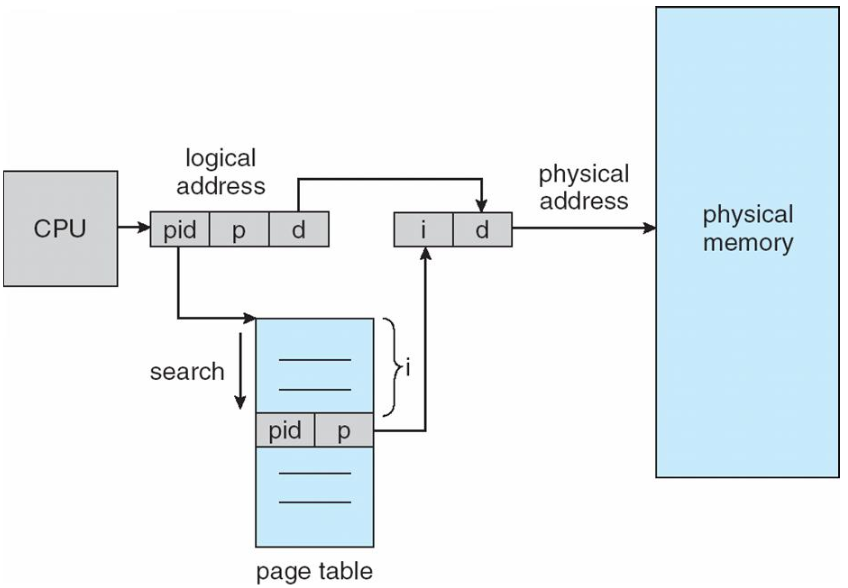
\includegraphics[width=1\linewidth]{content/OS_Internals/img/sfb.png}


    \end{minipage}
  \end{minipage}
\end{center}



Riduce la memoria necessaria per memorizzare ogni tabella delle pagine, ma aumenta
il tempo necessario per ricercare nella tabella quando si verifica un riferimento a una pagina.

Una soluzione potrebbe essere usare l'hashing per limitare la ricerca a una sola voce; anche il TLB può accelerare l'accesso.


\begin{figure}
  \centering
  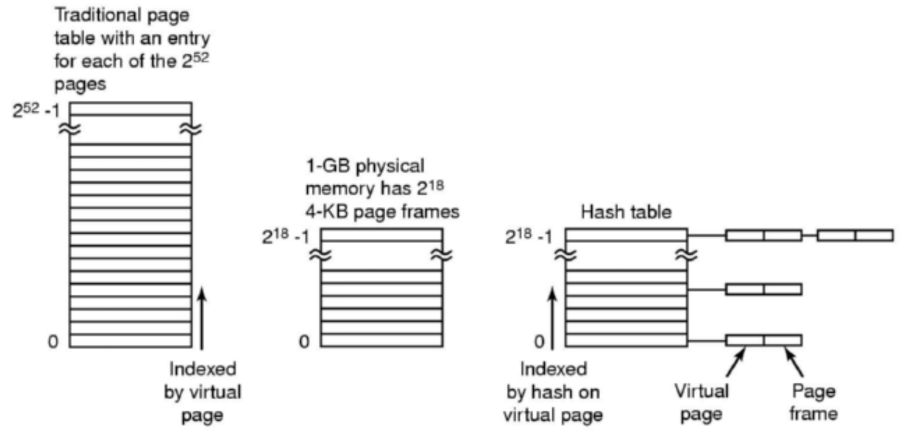
\includegraphics[width=0.5\linewidth]{images/OS_internals/Main-memory/MM-esempio2.png}
  \caption{Comparativa tra tabella delle pagine tradizionale e tabella delle pagine invertita}
\end{figure}

\section{Oracle SPARC Solaris}

Oracle SPARC Solaris è un sistema a 64-bit che è molto vicino e integrato con l'hardware.
È basato su due hash table:
\begin{itemize}
  \item Una per il kernel
  \item Una per i processi utente.
\end{itemize}

Ogniuna mappa memoria virtuale a memoria fisica. Più efficiente che avere due separate hash table per pagina.

Ogni entry ha un address e una span, che indica il numero di pagine che la entry rappresenta.\newline

TLB possiede la translation table entries (TTEs), per un accesso hardware più rapido.
La cache di TTEs risiede nel transaltion storage buffer (TSB), includendo un entry per le pagine recentemente accedute.\newline

Virtual address reference causa una TLB search:

Se è miss, l'hardware va a cercare nella memoria TSB guardando dentro la TTE corrispondente all'address.
\begin{itemize}
  \item Se è hit, la CPU copia la TSB entry nella TLB e la traduzione viene completata
  \item Se no match, il kernel interrompe la ricerca nella hash table. Il kernel crea una TTE dall'appropriata hash table e la memorizza nella TSB, Interrupt handler ritorna il controllo alla MMU, la quale completa la traduzione dell'address.

\end{itemize}


\section{Segmentazione}


\begin{center}
  \centering
  \begin{minipage}{1\linewidth}
    % Primo blocco: 50% dello spazio per il codice
    \begin{minipage}{0.65\linewidth}

      L'uso di pagine di dimensioni fisse apre il problema della frammentazione interna: ogni processo viene abbinato a un certo numero di pagine piuttosto che alla memoria di cui ha bisogno.

      Esiste quindi un modo per assegnare esattamente la quantità di memoria di cui un processo ha bisogno, evitando così qualsiasi spreco di memoria? La risposta è usare la \textbf{segmentazione}.

    \end{minipage}% <-- IMPORTANTE: il simbolo % qui evita spazi bianchi extra
    \hfill
    \begin{minipage}{0.3\linewidth}
      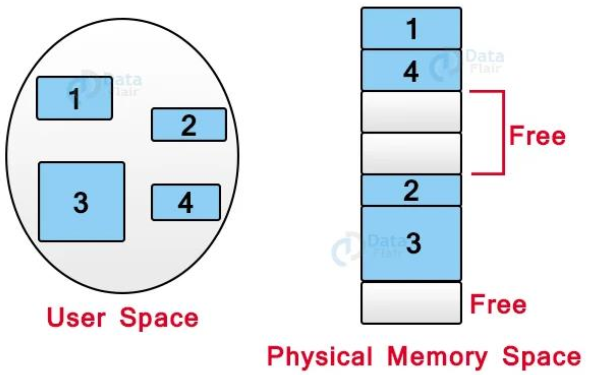
\includegraphics[width=1\linewidth]{content/OS_Internals/img/sdavg.png}


    \end{minipage}
  \end{minipage}
\end{center}

Un processo è diviso in blocchi; i blocchi in cui viene suddiviso un programma, che non devono essere necessariamente tutti della stessa dimensione, sono chiamati segmenti.

\begin{itemize}
  \item[--] Un blocco per lo stack
  \item[--] Un blocco per lo heap
  \item[--] Un blocco per la libreria 1
\end{itemize}

Ogni processo è diviso in diversi segmenti, tutti caricati in memoria durante l'esecuzione, anche se non necessariamente in modo contiguo.

Una tabella memorizza le informazioni su tutti questi segmenti: la base e il limite (lunghezza).


\begin{center}
  \centering
  \begin{minipage}{0.85\linewidth}
    % Primo blocco: 50% dello spazio per il codice
    \begin{minipage}{0.47\linewidth}

      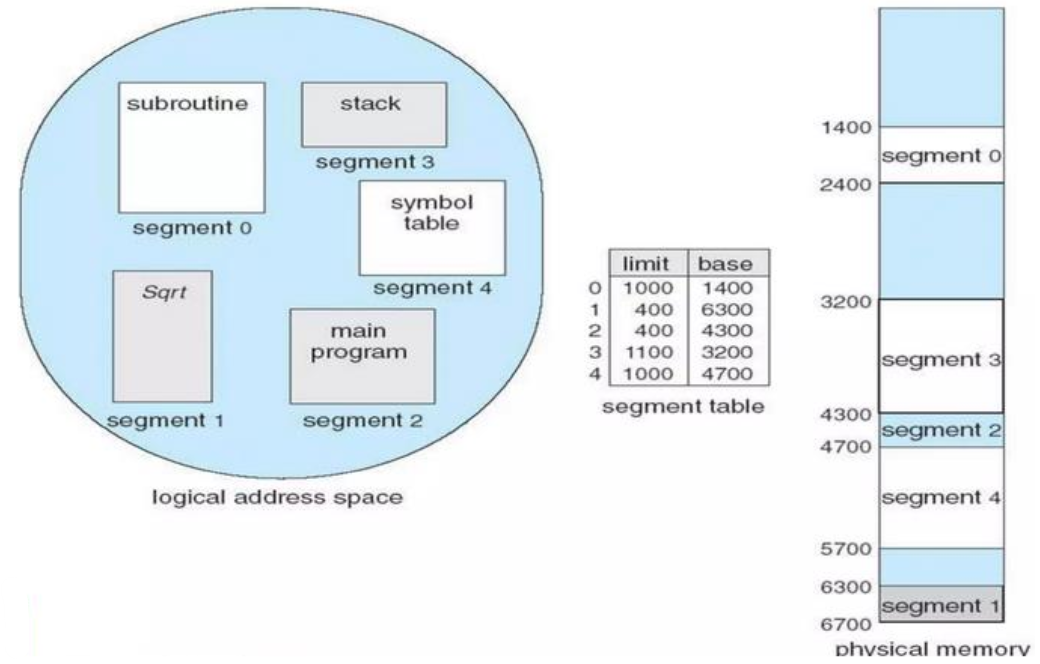
\includegraphics[width=1\linewidth]{content/OS_Internals/img/dgn.png}

    \end{minipage}% <-- IMPORTANTE: il simbolo % qui evita spazi bianchi extra
    \hfill
    \begin{minipage}{0.47\linewidth}
      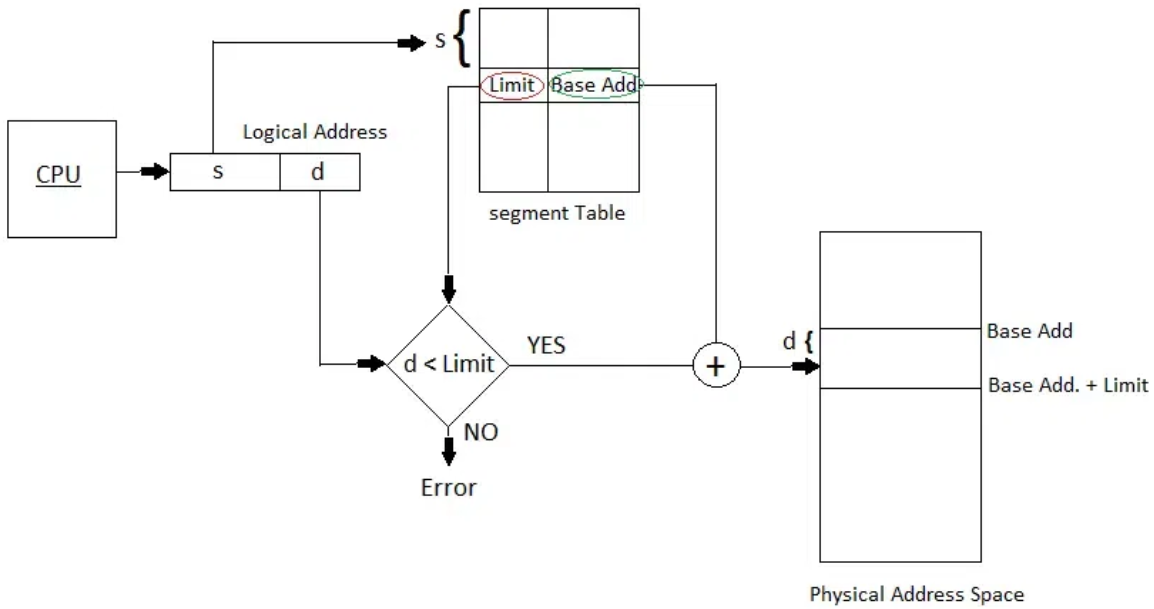
\includegraphics[width=1\linewidth]{content/OS_Internals/img/dasv.png}
      \captionof{figure}{Segmentazione: da logico a fisico}

    \end{minipage}
  \end{minipage}
\end{center}

\newpage
\subsection{Paginazione vs Segmentazione}

\begin{figure}[htbp]
  \centering
  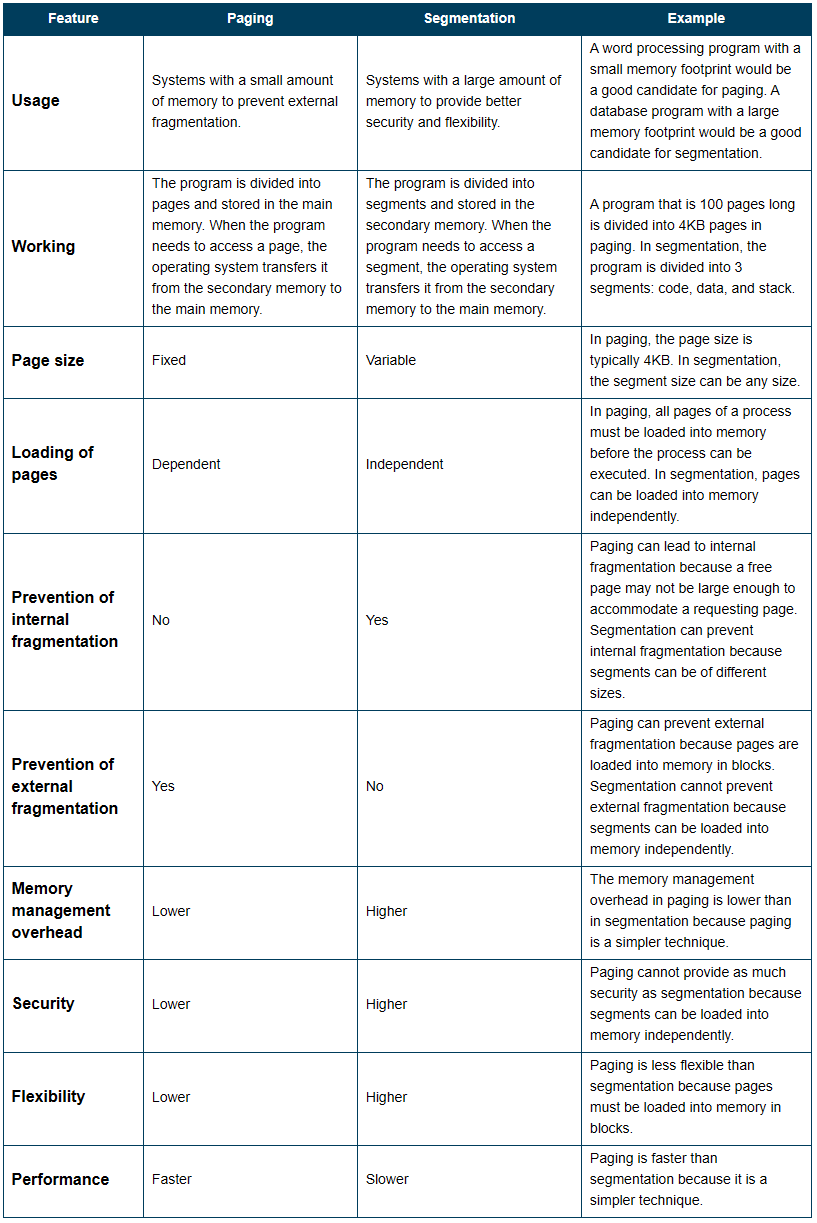
\includegraphics[width=0.9\linewidth]{content/OS_Internals/img/dsfb.png}
\end{figure}

\newpage
\begin{figure}[htbp]
  \centering
  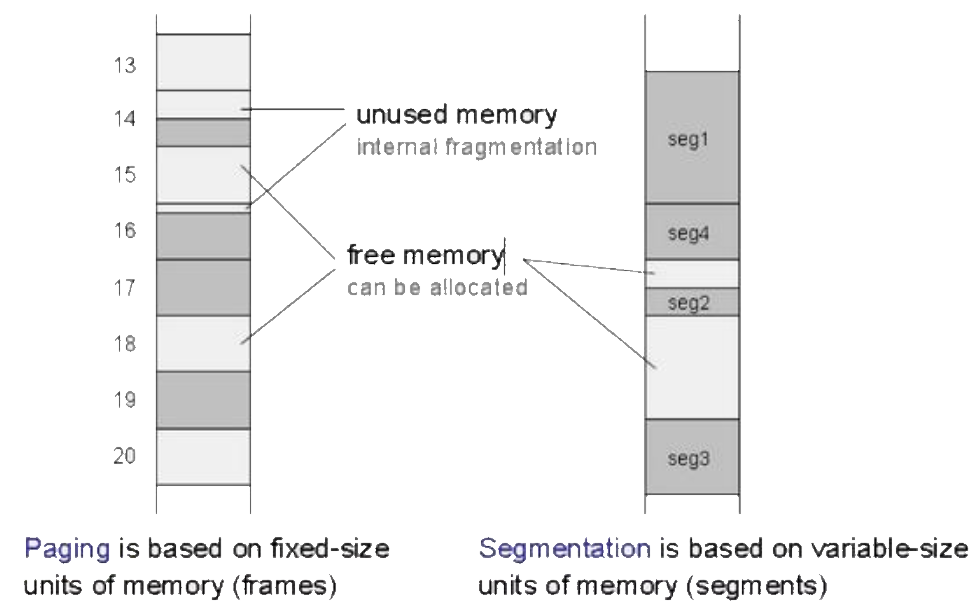
\includegraphics[width=0.5\linewidth]{content/OS_Internals/img/Immagine 2024-05-22 170639.png}
\end{figure}

\subsubsection{Esempio di Architettura Intel IA-32}

Lascia stare.

\begin{center}
  \centering
  \begin{minipage}{\linewidth}
    % Primo blocco: 50% dello spazio per il codice
    \begin{minipage}{0.5\linewidth}

      Le unità di paginazione formano l'equivalente dell'MMU; le dimensioni delle pagine possono essere 4 KB o 4 MB, con tabelle delle pagine a due livelli.

    \end{minipage}% <-- IMPORTANTE: il simbolo % qui evita spazi bianchi extra
    \hfill
    \begin{minipage}{0.4\linewidth}
      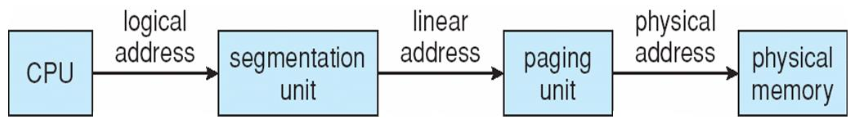
\includegraphics[width=1\linewidth]{content/OS_Internals/img/dddbv.png}

      \captionof{figure}{Conversione degli indirizzi di memoria}

      \vspace{0.1cm}

      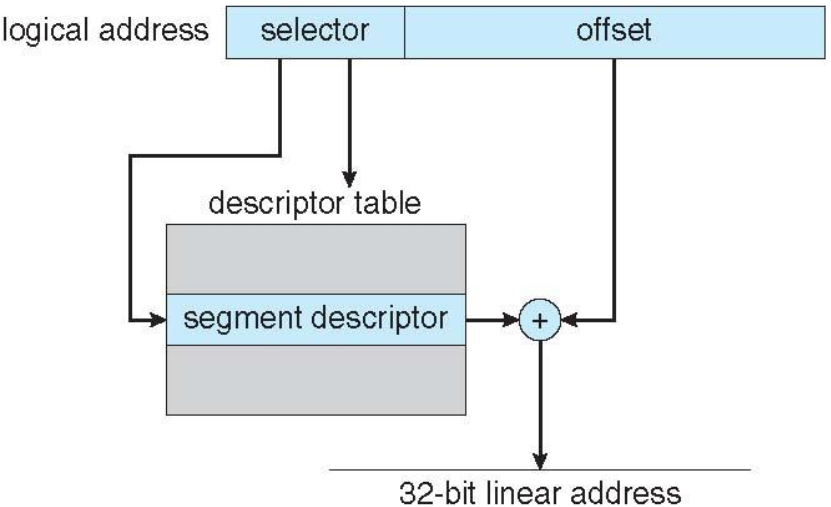
\includegraphics[width=1\linewidth]{content/OS_Internals/img/abdv.png}

    \end{minipage}
  \end{minipage}
\end{center}


\subsubsection{Esempio di Intel x86-64}

L'attuale generazione dell'architettura CISC ha 64 bit, il che è enorme (> 16 exabyte). In pratica viene implementato solo l'indirizzamento a 48 bit.

\begin{figure}[htbp]
  \centering
  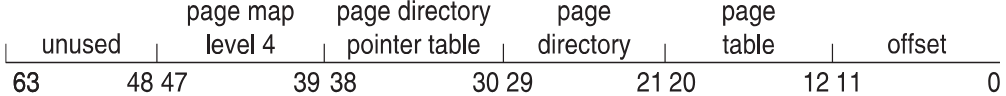
\includegraphics[width=0.8\linewidth]{content/OS_Internals/img/fmhh.png}
\end{figure}


\section{Esempio: Architettura ARM}

Nei moderni processori ARM installati sugli smartphone sono CPU 64bit con particolare attenzione ai consumi energetici.
Un livello di paginazione per sezione, due livelli si pagine più piccole.

\begin{minipage}{0.95\linewidth}
  % Primo blocco: 50% dello spazio per il codice
  \begin{minipage}{0.65\linewidth}

    Due livelli di TLBs

    \begin{itemize}
      \item L'outer ha due micro TLBs, uno per le istruzioni e uno per i dati.
      \item L'inner è una TLB singola
      \item Viene controllato il primo interno, successivamente vengono controllati gli esterni mancanti,
            e in caso di mancata corrispondenza viene eseguita la ricerca nella tabella delle pagine
            da parte della CPU.
    \end{itemize}

  \end{minipage}% <-- IMPORTANTE: il simbolo % qui evita spazi bianchi extra
  \hfill
  \begin{minipage}{0.3\linewidth}

    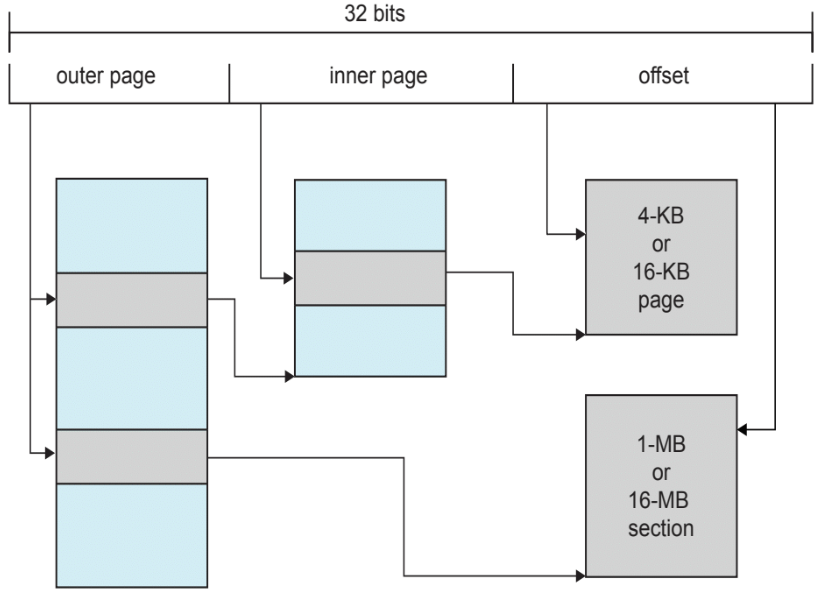
\includegraphics[width=1\linewidth]{images/OS_internals/Main-memory/MM-esempio3.png}
    \captionof{figure}{Architettura ARM}

  \end{minipage}
\end{minipage}
